%!TEX TS-program = xelatex
%!TEX encoding = UTF-8 Unicode

\documentclass[
	12pt,
	twoside,
	openright
	]{book}

\usepackage[
	top=1in,
	bottom=1.2in,
	inner=1.2in,
	%margin=1.23in,
	textwidth=12cm,
	%right=7cm,
	%showframe
	]{geometry}

\geometry{a4paper}

%\usepackage[parfill]{parskip}
\usepackage{graphicx}
\usepackage{epstopdf}
\epstopdfsetup{update}
\usepackage[usenames]{color}
% \usepackage{amssymb}
\usepackage{amsmath}

\usepackage{pdfpages}

\usepackage{titlesec}
\usepackage{titling}
\usepackage{titletoc}

\usepackage[hang,flushmargin]{footmisc}

\newcommand{\hsp}{\hspace{19pt}}
\titleformat{\chapter}[hang]{\Huge\bfseries}{\thechapter\hsp•\hsp}{0pt}{\Huge\bfseries}

\usepackage{listings}

\usepackage{Alegreya}
\linespread{1.2}
\usepackage{
	fontspec,
	xltxtra,
	xunicode
	}

\usepackage{
	xfrac,
	unicode-math
	}

\defaultfontfeatures{Mapping=tex-text}
\setmonofont[
	Scale=MatchLowercase
	]{Andale Mono}
\setmathfont[
	Scale=MatchLowercase,
	Scale=1
	]{Libertinus Math}
\setsansfont[
	Scale=MatchLowercase,
	Mapping=tex-text
	]{Alegreya Sans}

\newfontfamily\quotefont[
	Scale=MatchLowercase,
	Mapping=tex-text,
	LetterSpace=5.0,
	%Scale=1.123,
	]{Alegreya Sans}%{Open Sans Light}%{Fira Sans Light}

\usepackage{etoolbox}
\AtBeginEnvironment{quote}{\quotefont\small}

\usepackage[
	autostyle,
	italian=guillemets,
	% altre opzioni
	]{csquotes}

\usepackage[
	english,
	italian
	]{babel}

\usepackage{imakeidx}
\makeindex[name=names, title=Indice dei nomi]
\makeindex[name=things, title=Indice analitico]

\usepackage{tabularx}
\usepackage{array}
\newcolumntype{L}[1]{>{\raggedright\let\newline\\\arraybackslash\hspace{0pt}}m{#1}}
\newcolumntype{C}[1]{>{\centering\let\newline\\\arraybackslash\hspace{0pt}}m{#1}}
\newcolumntype{R}[1]{>{\raggedleft\let\newline\\\arraybackslash\hspace{0pt}}m{#1}}

\usepackage{longtable}
\usepackage{multirow}
\usepackage{booktabs}

\usepackage{paralist}

\usepackage{tikz}
\usetikzlibrary{
  angles,
  quotes,
  decorations.pathmorphing,
  decorations.markings}
\usepackage{pgfplots}

\usepackage{wrapfig}
\usepackage{setspace}
\usepackage[%
  margin=10pt,
	labelfont=bf,
	labelsep=endash,
]{caption}
\captionsetup{font={sf,footnotesize,stretch=0.98}}

\usepackage{subcaption}

\usepackage{float}
%\floatstyle{boxed}
\restylefloat{figure}

\usepackage{url}

\renewcommand{\arraystretch}{1.6}

\newfontfamily\csdb[Ligatures=TeX]{Alegreya}

\usepackage{changepage}

%\usepackage{ragged2e}

\usepackage[
	%style=authoryear,
	%backend=biber
]{biblatex}

\addbibresource{musebib/nono-luigi.bib}
\addbibresource{musebib/novecento.bib}
\addbibresource{smc2020bib.bib}
\addbibresource{microfoni.bib}
%\addbibresource{musebib/partiture/milestone.bib}

% ----------------------------------------------------–––––––––– LISTING

% Make LaTeX output a dot when typing an asterisk
%\DeclareMathSymbol{*}{\mathbin}{symbols}{"01}

% lstlistings setup
\definecolor{yobg}{rgb}{0.9,0.9,1}
\definecolor{yotxt}{rgb}{0.01,0.01,0.52} % a dark blue.
\definecolor{mylstbg}{rgb}{0.98,0.98,0.98} % a really pale grey.
\definecolor{mylstcmt}{rgb}{0.01,0.52,0.01} % a dark green.
\definecolor{mylstdoc}{rgb}{0.80,0.30,0.80} % a medium pink.

\lstset{%
  aboveskip=20pt,
	belowskip=15pt,
  language=C++,
  numbers=left,%none,
  tabsize=2,
  %frame=single,
  breaklines=false,
  numberstyle=\tiny\ttfamily,
  backgroundcolor=\color{mylstbg},
  basicstyle=\footnotesize\ttfamily,
  commentstyle=\slshape\color{mylstcmt}, %\itshape,
  %frameround=tttt,
  columns=flexible, %fixed,
  showstringspaces=false,
  emptylines=2,
  inputencoding=utf8,
  extendedchars=true,
  emph={component, declare, environment, import, library, process},
  emph={[2]ffunction, fconstant, fvariable},
  emph={[3]button, checkbox, vslider, hslider, nentry, vgroup, hgroup, tgroup, vbargraph, hbargraph, attach},
  emphstyle=\color{yotxt}, %\underline, %\bfseries,
  morecomment=[s][\color{mylstdoc}]{<mdoc>}{</mdoc>},
  rulecolor=\color{black}
}

% ----------------------------------------------------–––––––––– CUSTOM COMMANND
\newcommand*\rfrac[2]{{}^{#1}\!/_{#2}}

\newcommand{\adb}{\index[names]{Blumlein, Alan Dower}\emph{Alan D. Blumlein}}
\newcommand{\mg}{\index[names]{Gerzon, Michael}\emph{Michael Gerzon}}

\newcommand{\rb}{\index[things]{Rumore Bianco}\emph{rumore bianco}}
\newcommand{\tz}{\index[things]{Trasformata zeta}\emph{trasformata zeta}}

\usepackage[framemethod=tikz]{mdframed} % Allows defining custom boxed/framed environments

%-------------------------------------------------------------------------------
%--------------------------------------------------- INFORMATION ENVIRONMENT ---
%-------------------------------------------------------------------------------

% Usage:
% \begin{info}[optional title, defaults to "Info:"]
% 	contents
% 	\end{info}

\mdfdefinestyle{info}{%
	topline=false, bottomline=false,
	leftline=false, rightline=false,
	nobreak,
	singleextra={%
		\fill[black](P-|O)circle[radius=0.4em];
		\node at(P-|O){\color{white}\scriptsize\bf i};
		\draw[very thick](P-|O)++(0,-0.8em)--(O);%--(O-|P);
	}
}

% Define a custom environment for information
\newenvironment{info}[1][Info:]{ % Set the default title to "Info:"
	\medskip
	\begin{mdframed}[style=info]
		\noindent{\textbf{#1}}
}{
	\end{mdframed}
}

%-------------------------------------------------------------------------------
%----------------------------------------------------- BIOGRAFIA ENVIRONMENT ---
%-------------------------------------------------------------------------------

% Usage:
% \begin{bio}[optional title, defaults to "Info:"]
% 	contents
% 	\end{bio}

\mdfdefinestyle{bio}{%
	topline=false, bottomline=false,
	leftline=false, rightline=false,
	nobreak,
	singleextra={%
		\fill[black](P-|O)circle[radius=0.4em];
		\node at(P-|O){\color{white}\scriptsize\bf b};
		\draw[very thick](P-|O)++(0,-0.8em)--(O);%--(O-|P);
	}
}

% Define a custom environment for information
\newenvironment{bio}[1][Biografia:]{ % Set the default title to "Info:"
	\medskip
	\begin{mdframed}[style=bio]
		\noindent{\textbf{#1}}
}{
	\end{mdframed}
}

%-------------------------------------------------------------------------------
%------------------------------------------------------- WARNING ENVIRONMENT ---
%-------------------------------------------------------------------------------

% Usage:
% \begin{warn}[optional title, defaults to "Warning:"]
%	Contents
% \end{warn}

\mdfdefinestyle{warning}{
	topline=false, bottomline=false,
	leftline=false, rightline=false,
	nobreak,
	singleextra={%
		\draw(P-|O)++(-0.5em,0)node(tmp1){};
		\draw(P-|O)++(0.5em,0)node(tmp2){};
		\fill[black,rotate around={45:(P-|O)}](tmp1)rectangle(tmp2);
		\node at(P-|O){\color{white}\scriptsize\bf !};
		\draw[very thick](P-|O)++(0,-1em)--(O);%--(O-|P);
	}
}

% Define a custom environment for warning text
\newenvironment{warn}[1][Warning:]{ % Set the default warning to "Warning:"
	\medskip
	\begin{mdframed}[style=warning]
		\noindent{\textbf{#1}}
}{
	\end{mdframed}
}

%-------------------------------------------------------------------------------
%------------------------------------------------------------ BEGIN DOCUMENT ---
%-------------------------------------------------------------------------------

\begin{document}

%%!TEX TS-program = xelatex
%!TEX encoding = UTF-8 Unicode
%!TEX root = ../../../LSSN.tex

%------------------------- COMANDO TIKZ
\newcommand\Base[1][0]{
\begin{scope}[xshift=#1]
\clip
  (-0.5,5.5) rectangle (5.5,-0.5);
  \draw[->]
  (-0.5,0) -- (5,0) node[right] {$u$};
\draw[->]
  (0,-0.5) -- (0,5) node[above] {$v$};
\coordinate (O) at (0,0);
\coordinate (aux1) at (40:4);
\coordinate (aux2) at (aux1|-0,0);
\coordinate (aux3) at (4,{4*tan(40)});
\draw
  (O) -- (aux3) -- (aux3|-0,0)
  (aux1) -- (aux2);
\draw[
	thick,
	%red!70!black
	]
  (O) circle (4);
\pic[
	draw,
	"$x$",
	angle radius=30pt,
	angle eccentricity=1.2
	]{angle = aux2--O--aux1};
\end{scope}
}
%------------------------- COMANDO TIKZ


%!TEX TS-program = xelatex
%!TEX encoding = UTF-8 Unicode
% !TEX root = ../METM.tex

%------------------------- COPERTINA
\begin{center}
	\fontsize{40}{40}{\csdb MUSICA} \\
	\fontsize{40}{40}{\csdb ELETTRONICA} \\
	\fontsize{40}{40}{\csdb TECNOLOGIA} \\
	\fontsize{40}{40}{\csdb MUSICALE}\\[-.31cm]
	\noindent\makebox[\linewidth]{\rule{.51\paperwidth}{1pt}}
	%\fontsize{19}{19}\selectfont{Pasquale CITERA} 	\\
	%\fontsize{19}{19}\selectfont{Marco Matteo MARKIDIS} 	\\
	\fontsize{19}{19}\selectfont{Giuseppe SILVI} 	\\
	\vfill
	\fontsize{13}{13}\selectfont{APPUNTI} \\
	%\fontsize{13}{13}\selectfont{Liceo Musicale S. SATTA di NUORO} \\
	\fontsize{13}{13}\selectfont{\emph{draft - \today}} \\
\end{center}
\thispagestyle{empty}
\clearpage
~ \vfill
blank page
\thispagestyle{empty}
\clearpage
%------------------------- COPERTINA


\clearpage

\tableofcontents

%\raggedright

%!TEX TS-program = xelatex
%!TEX encoding = UTF-8 Unicode
% !TEX root = ../metp.tex

\chapter*{MANIFESTO}
\addcontentsline{toc}{chapter}{MANIFESTO}

%\begin{adjustwidth}{23mm}{0mm}

Questo lavoro deriva dall'esigenza di organizzare un testo che possa
ristabilire un equilibrio scolastico e, con un po' di presunzione, artistico,
nelle attività didattiche inerenti la Musica Elettronica e le Tecnologie
Musicali. Non è propriamente un manuale quanto una raccolta organizzata di
appunti che seguano un percorso chiaro e progressivo attraverso gli anni di
studio della materia.

L'esigenza di mettere in un contenitore questi materiali viene direttamente
dal percorso d'insegnamento in diversi gradi del percorso formativo elettroacustico.
La bibliografia specifica è ricca ed in continua evoluzione data la materia
viva che la alimenta. Nonostante questo, in lingua italiana, i testi attualmente di
riferimento hanno un assetto ludico, d'intrattenimento. Organizzati ad
unità come fossero un corso di lingua, a livelli, trasformano argomenti musicali
in attitudini ricreative, rafforzando l'idea di didattica applicata alla base
di troppe classi di musica elettronica in Italia.

Un riferimento letterario, ad indirizzo opposto, è il testo di Walter Branchi
\emph{Tecnologia della Musica Elettronica} che dal lontano 1975 ancora riesce
a suggerire un'idea di didattica organica e progressiva ineguagliata, con i
difetti di un'opera prima in tutti i sensi, ma con la prospettiva dello studio
scolastico organizzato. A questo testo si ispira questa raccolta, \emph{METP},
all'idea di un percorso di comprensione che viene da un'idea di scuola,
senza la pretesa di creare un abile manovratore di pomelli in ogni possibile lettore.
Le problematiche essenziali sono altre e sono, sempre prendendo spunto dal lavoro di Branchi,
ancora egregiamente espresse dalle parole di Domenico Guaccero nella prefazione:

\begin{quote}
  \ldots val la pena ricordare e mantenere fermi gli apporti che la “musica
  elettronica” ha introdotto nell'opera musicale\ldots E cioè l'andare alla
  radice del suono, come fatto fisico e (ache) da qui come fatto musicale, la
  possibilità di liberarsi definitivamente dal “dover costruire” sitemi
  intervallari, il porre il problema del rapporto musica esecutore e musica
  spettacolo in termini fino allora inusitati, di riproporre, ma allargandone
  permamentemente i confini, il rapporto tra tecnologia e composizione.
\end{quote}

In questa ottica di indagine, alla \emph{radice del suono}, ci si pone
trasversalmente, lungo il periodo d'apprendimento di uno studente, a qualsiasi
livello. Non è dunque la quantità di nozioni (o unità) che si collezionano con
la lettura, quanto la qualità dell'esperienza formativa a tracciare il percorso.

\begin{quote}
  Cominciare con uno studio del “tempo” e delle "onde"\ldots È li che comincia
  il moto, quindi il suono. È li che musicista e tecnico cominciano ad
  incontrarsi. Prima di tutte le cognizioni di acustica ed elettroacustica o di
  tecnologia elettronica, è li che si può misurare quello che diventa il "nuovo"
  tecnico-musicale itrodotto tramite i mezzi elettronici: com'è stato detto, si
  tratta di "comporre il suono, non comporre col suono".
\end{quote}

La composizione come materia di studio sembra non appartenere più alle classi di
tecnologia. Il mezzo tecnico ha completamente inebriato le menti e distolto
l'attenzione dall'\emph{osservazione mediante composizione} di ciò che percepiamo,
ovvero, ancora: il suono. Uno studente agli inizi del proprio percorso potrebbe
affrontare un esercizio compositivo se gli si fornissero le regole di
comprensione del proprio operato e della relazione di questo con il mondo percepito, per

\begin{quote}
  \ldots andare alla radice del suono. In quest'ambito possono avere più senso
  i vari problemi, come quello di mirare a costruire timbri nuovi\ldots studiare
  per analisi, gli strumenti naturali, in maniera da usare gli strumenti naturali
  come termini di confronto cui l'orecchio è abituato, cioè scritti in codice
  forte.

  Dalla radice del suono, come fatto fisico, si può passare alla radice della
  percezione e della realizzazione sonora.
\end{quote}

Negli anni di scuola superiore, del Liceo, questa metodologia è adottata
\emph{naturalmente}. Sarebbe troppo semplice parlare di materie scientifiche
quali la fisica, la biologia, la chimica per creare paralleli tra percepito,
analizzato e compreso. Girandoci più alla larga possibile potremmo parlare di
latino e italiano, di letteratura. Di imparare a scrivere attraverso la storia
della scrittura, dei meccanismi che hanno resistito alla storia per finire nel
linguaggio comune. Nella musica elettronica, nelle tecnologie musicali, nei
libri ad unità, si procede per atemporalità, per meccanismi e tecnicismi avulsi
dall'essere nel tempo delle cose. Si spiegano le tecniche senza su queste fare
quello che si fa in italiano, scrivere, comporre temi. Come se la composizione
fosse una questione esclusiva dei compositori.

Insegnare a comporre, a scrivere, attraverso il ragionameto, è un esattamente
una questione tecnica

\begin{quote}
  faranno bene ad essere quanto più rigorosi teoriocamente e quanto più
  preparati tecnologicamente, in maniera da poter maneggiare tutte le
  apparecchiature possibili\ldots È la via della didattica, quella a cui
  intelligentemente si rifà questo libro di Branchi\ldots

  Esso non è un testo pensato a priori per insegnare le tecniche elettroniche,
  ma è \emph{il risultato} d'una attività didattica già effettuata\ldots Non
  un'aggiunta all'erudizione o un contributo all'indagine teorica, ma, più
  semplicemente e pertinemtemente, uno strumento di lavoro, da utilizzare nella
  pratica.
\end{quote}

Questo lavoro ha la presunzione di non servire a niente se lo scolpo della
lettura è un'apprendimento collezionistico di espedienti e meccanismi.

Questo lavoro vuole e può fornire meccanismi mentali di indagine,
sperimentazione, speculazione, comprensione e composizione che \emph{una scuola}
dovrebbe innestare in alcuni studenti, in alcuni individui. Non in tutti, come nei
corsi di lingua di base, una unità alla volta, ma solo quelli che da questi
ragionamenti possano alzare gli occhi per scoprire di aver
cambiato il proprio modo di percepire le relazioni tra le cose.

***

Questo testo, pur prendendo prezioso esempio dalle pagine di Branchi, vuole fare
diversi passi in molteplici altre direzioni. La distanza temporale dal testo di
Branchi ci permette di guardare a nuovi modi di fare didattica. Il più
importante ed efficae è quello del libero accesso al codice, alla libera
partecipazione al progetto per un'informazione aperta alla discussione.

Questo testo è quindi open source, il progetto risiede all'indirizzo
\url{https://github.grammaton.io/metp}. Atteaverso questo indirizzo si può
partecipare alla scrittura, all'integrazione, alla discussione al fine di
rendere il testo vivo, in continua composizione.

Please note that this project is released with a Contributor Code of Conduct.
By participating in this project you agree to abide by its terms.

%\end{adjustwidth}

\clearpage


\input{CAPITOLI/0001-COC}

%!TEX TS-program = xelatex
%!TEX encoding = UTF-8 Unicode
% !TEX root = ../../metp.tex

\chapter{FENOMENI}
\startcontents[chapters]
\printcontents[chapters]{}{1}{}

~\vfill

\begin{flushright}
		\textit{Nihil est in intellectu quod prius non fuerit in sensu}\footnote{
		Locuz. lat. \emph{niente è nell’intelletto, che prima non sia stato nei sensi},
		usata come assioma nella filosofia scolastica. Accolta da Locke nella
		sua teoria sull’origine delle idee, fu integrata da Leibniz con
		l’aggiunta \emph{nisi ipse intellectus} \emph{(eccetto l’intelletto stesso)}. --
		\url{treccani.it}}
	\end{flushright}

\bigskip

Il \emph{primo passo} che l'uomo compie, ciclicamente, verso la comprensione del
mondo sonoro che lo circonda è cambiato innumerevoli volte durante la storia degli
ultimi 3000 anni ed è sempre stato un passo mosso di pari passo con la musica,
la sua storia, la sua funzione culturale.

In Europa, solo nel novecento, possiamo segnalare differenti approcci alla
comprensione del mondo sonoro prima e dopo le guerre, prima e dopo la radio-televisione,
prima e dopo il calcolatore digitale, prima e dopo l'automobile come bene primario.

%Varese:
%Turing:

Oggi si può ascoltare e cominciare a parlare di suono cercando di unire discipline diverse
che trattano il tema scientificamente, tra cui, la musica, ormai è una di queste.
Il primo oggetto analizzabile da questo punto di vista è proprio l'oscillazione nel tempo,
il moto che da vita alla materia in vibrazione.

\clearpage

%!TEX TS-program = xelatex
%!TEX encoding = UTF-8 Unicode
%!TEX root = ../../metm.tex

\section{Oscillazioni}

Osservando, anche ad occhi chiusi, una ruota panoramica potremmo dire che
completa una rotazione ogni 30 minuti. Osservando ancora il comportamento di
questa ruota panoramica notiamo che questa compie un giro ogni 30 minuti,
ovvero completa un ciclo di rotazione tornando al punto di partenza e poi
ripete questa rivoluzione più volte. Questo è un esempio di funzione periodica,
perché la ruota panoramica ripete la sua rivoluzione, o ciclo, ogni 30 minuti
e quindi diciamo che ha un periodo di 30 minuti.

\input{CAPITOLI/0100/TIKZ/0101-pan}

Osservate ancora la ruota panoramica, si muove in senso antiorario. C'è una
sola cabina occupata, seguiamola. Volendo prendere nota dell'altezza di quella
cabina durante i trenta minuti che impiega a tornare al punto di partenza,
seguendola disegneremmo una linea, probabilmente verticale, che va dall'altezza
minima all'altezza massima.

%!TEX TS-program = xelatex
%!TEX encoding = UTF-8 Unicode

%------------------------- IMMAGINE TIKZ
\begin{tikzpicture}[scale=.99]
  \draw[->] (0,-2.5) -- (0,2.5);
  \draw[->] (-2.5,0) -- (2.5,0);

\draw[
  postaction={
    decorate,decoration={
      markings,
      mark=at position 0.19 with {\arrow[line width=1mm]{>}},
      mark=at position 0.69 with {\arrow[line width=1mm]{>}}}},
    thick
] (0,0) circle (2);

\coordinate (A) at (2,0);

\filldraw (A) circle (2pt) node[above right] {00'};
\filldraw (A) circle (2pt) node[below right] {30'};

\coordinate (B) at (90 : 2);

\filldraw (B) circle (2pt) node[above left] {Cabina};

\draw (4,-2) -- (4,2);

\coordinate (C) at (4,0);
\coordinate (D) at (4,2);
\coordinate (F) at (4,-2);

\filldraw (C) circle (2pt) node[above right] {0};
\filldraw (D) circle (2pt) node[above right] {altezza massima};
\filldraw (F) circle (2pt) node[below right] {altezza minima};

\coordinate (E) at (270 : 2);

\filldraw (E) circle (2pt) node[below right] {Cabina};

\draw[dashed] (0,2) -- (4,2);
\draw[dashed] (0,-2) -- (4,-2);
\end{tikzpicture}
%------------------------- IMMAGINE TIKZ


Se decidessimo che il nostro foglio avesse non una, come nella descrizione
precedente, ma due dimensioni di rappresentazione, l'altezza ed il tempo, e
quindi seguissimo con lo sguardo la cabina ed annotando l'altezza spostassimo
simultaneamente ed a velocità costante il foglio, simulando lo scorrimento del
tempo, il disegno finale dovrebbe apparire come un'onda.

\input{CAPITOLI/0100/TIKZ/0103-pan}

Con la rappresentazione dell'onda descriviamo un'oscillazione, ovvero un moto
periodico attorno alla posizione di equilibrio.

Un altro fenomeno oscillatorio estremamente esemplificativo è quello del pendolo.

Da un punto di quiete il pendolo si muoverà nel tempo fino al suo massimo
spostamento per poi tornare al punto di partenza e ripetere un uguale movimento
in senso opposto.

Considerando un pendolo che si sposti da una parte all'altra rispetto alla sua
posizione di equilibrio anche il suo movimento oscillatorio nel tempo può essere
rappresentato come un'oscillazione.

%!TEX TS-program = xelatex
%!TEX encoding = UTF-8 Unicode
%!TEX root = ../../../LSSN.tex

%------------------------- IMMAGINE TIKZ
\begin{tikzpicture}[scale=.99]
  \draw[dashed] (0,-0.5) -- (0,0.5);
  \draw[->] (-0.5,0) -- (12,0);
       %\draw[thick] (0,0) circle (2);
       \draw[thick, ->] (45:2)arc(45:-45:2);
       \coordinate (origin) at (0:0);
       \coordinate (A) at (45:2);
       \coordinate (B) at (-45:2);
       \coordinate (0) at (0:2);
       \coordinate (1) at (7.071,1.414);
       \coordinate (-1) at (4.242,-1.414);
  \filldraw (A) circle (2pt) node[above right] {};
  \filldraw (0) circle (2pt) node[above right] {0};
  \filldraw (A) circle (5pt) node[above right] {};
  \draw (B) circle (5pt) node[above right] {};
  \draw[-] (origin) -- (A);
  \draw[dashed] (origin) -- (B);
  \draw[dashed] (B) -- (-1);
  \draw[dashed] (A) -- (1);
  \filldraw (1) circle (2pt) node[above] {};
  \filldraw (-1) circle (2pt) node[below] {};

  \draw[thick] (A) cos (2.828,0) sin (4.242,-1.414) cos (5.656, 0) sin (7.071,1.414) cos (8.485,0) sin (9.899,-1.414) cos (11.313,0);
\end{tikzpicture}
%------------------------- IMMAGINE TIKZ


L'oscillazione rappresentata da un moto di questo tipo è definita moto armonico
semplice o sinusoidale.

Definiamo una quantità in oscillazione quando il suo valore si muove con
continuità passando tra un massimo ad un minimo.

\clearpage

\section{Le grandezze di un'oscillazione}

La rappresentazione di un fenomeno oscillatorio ci permette di descrivere
quali siano le grandezze principali:

\begin{compactitem}
	\item ampiezza
	\item frequenza
	\item periodo
	\item fase (da spiegare)
	\item lunghezza d'onda (da spiegare)
	%\item pulsazione
\end{compactitem}

Definiamo \textbf{ampiezza} di un'oscillazione il massimo valore raggiunto
dal suo valore di equilibrio.

Facendo riferimento al movimento del pendolo, diciamo che la distanza massima
raggiunta nel suo movimento da una parte all'altra rispetto alla posizione di
equilibrio definisce la sua ampiezza di oscillazione.

%!TEX TS-program = xelatex
%!TEX encoding = UTF-8 Unicode
%!TEX root = ../../../LSSN.tex

%------------------------- IMMAGINE TIKZ
\begin{tikzpicture}[scale=.99]
  \draw[->] (1.414,-2) -- (1.414,2);
  \draw[->] (0.914,0) -- (12,0);
       \coordinate (origin) at (0:0);
       \coordinate (A) at (45:2);
       \coordinate (B) at (-45:2);
       \coordinate (0) at (0:2);
       \coordinate (1) at (7.071,1.414);
       \coordinate (-1) at (4.242,-1.414);
  \filldraw (A) circle (2pt) node[above right] {};
  \draw[dashed] (B) -- (-1);
  \draw[dashed] (A) -- (1);
  \filldraw (1) circle (2pt) node[above] {};
  \filldraw (-1) circle (2pt) node[below] {};

  \draw[thick] (1.414,1.414) cos (2.828,0) sin (4.242,-1.414) cos (5.656, 0) sin (7.071,1.414) cos (8.485,0) sin (9.899,-1.414) cos (11.313,0);

  \draw[thick] (4.242,-1.414) -- (4.242,0) node[above] {$a$};
  \draw[thick] (7.071,1.414) -- (7.071,0) node[below] {$a$};
\end{tikzpicture}
%------------------------- IMMAGINE TIKZ


Definiamo \textbf{frequenza} il numero di ripetizioni nell'unità di tempo. La
frequenza di oscillazione di un pendolo corrisponde al numero di volte che questo
torna alla posizione di partenza dopo aver percorso l'intero tragitto ondulatorio.
Nell'immagine della ruota panoramica la frequenza descrive quanti giri essa realizza
nell'unità di tempo prestabilita.

Descriviamo quindi con il valore di \textbf{frequenza} di un'oscillazione il
\emph{numero di cicli per secondo (cps)}. L'unità di misura della frequenza è
\emph{Hertz (Hz)}.

\input{CAPITOLI/0100/TIKZ/0106-freq}

Il \emph{ciclo} o \textbf{periodo} di un'oscillazione rappresenta la durata di
una singola oscillazione alla frequenza data.
Il legame tra frequenza e periodo è tale che all'aumentare della frequenza
diminuisce la durata, e quindi il periodo, nel rapporto di $T = 1/f$ dove
$T$ è la durata del periodo espressa in secondi.

Considerando quindi il \emph{secondo} un intero divisibile in parti uguali,
definiamo con $f$ la \emph{frequenza}, ovvero il numero di parti e con $T$
il \emph{periodo} ovvero la durata di una singola parte. La durata della
singola parte moltiplicata per il numero delle parti ri-compone l'intero \emph{secondo}.

\bigskip

%------------------------- APPROFONDIMENTO
		\begin{tabular}{L{.969\textwidth}}%
		\toprule
			\textbf{Hertz}\\
		\midrule
			Unità di misura della frequenza dei fenomeni periodici; un fenomeno ha
			frequenza 1 \emph{Hertz} se un suo periodo dura 1 secondo; simbolo
			\emph{Hz}.\\

			DATA 1937.\\

			ETIMOLOGIA Dal nome del fisico tedesco Heinrich Rudolf Hertz (1857–94),
			Fisico tedesco e pioniere della comunicazione radio. Ha proseguito il
			lavoro di Maxwell sulle onde elettromagnetiche e fu il primo a trasmettere
			e ricevere onde radio. Hertz ha anche dimostrato che la luce ed il calore
			radiante hanno natura elettromagnetica. \\
		\bottomrule
		\end{tabular}
%------------------------- APPROFONDIMENTO

\clearpage

\section{Oscillazione Sinusoidale}

%------------------------- APPROFONDIMENTO
		\begin{tabular}{L{.969\textwidth}}%
		\toprule
			\textbf{Sinusoide} \\
		\midrule
			In geometria: curva sinusoide (o la sinusoide s.f.), la curva che, in
			coordinate cartesiane ortogonali, rappresenta il diagramma della funzione
			seno, tipico dei fenomeni periodici senza smorzamento. \\

			DATA 1895.\\

			ETIMOLOGIA Der. del lat. \emph{sinus -us} ‘seno’, col suff. \emph{-oide}.\\
		\bottomrule
		\end{tabular}
%------------------------- APPROFONDIMENTO

% \input{CAPITOLI/0100/TIKZ/0107-cos}
%
% Potremmo rapidamente intuire la connessione  con il cerchio unitario, poiché
% l'altezza della cabina corrisponderebbe al valore $ y $ di un punto sul cerchio.
% Possiamo determinare il valore di $ y $ usando la funzione seno. Per avere
% un'idea migliore del comportamento di questa funzione, possiamo creare una
% tabella di valori che conosciamo e usarli per tracciare un grafico delle
% funzioni seno e coseno.
%
% %!TEX TS-program = xelatex
%!TEX encoding = UTF-8 Unicode
%!TEX root = ../../../LSSN.tex

%------------------------- IMMAGINE TIKZ
\begin{tikzpicture}[scale=.99]

    \draw[->] (0,-3) -- (0,3);
    \draw[->] (0,0) -- (12,0);
    \foreach \x in {1,2,3,4,5,6,7,8,9,10,11}
        \draw (\x,2pt) -- (\x,-2pt);
    \foreach \y in {-2,-1,0,1,2}
        \draw (2pt,\y) -- (-2pt,\y);

\coordinate (A) at (8,2);
\coordinate (B) at (4,-2);
\filldraw (A) circle (2pt) node[above] {{$\frac{\pi}{2}$}};
\filldraw (B) circle (2pt) node[below] {{{$\frac{\sqrt2}{2}$}}};

   \draw[dashed, gray] (0,-3) grid (12,3);
   %\draw[help lines] (0,-3) grid (12,3);
   \draw (0,2) cos (2,0) sin (4,-2) cos (6,0) sin (8,2) cos (10,0) sin (12,-2);
   %%\draw (0,0) to (12,0);
   \label{sin001}
\end{tikzpicture}
%------------------------- IMMAGINE TIKZ

%
% \input{CAPITOLI/0100/TIKZ/0109-sincos}
%
% 		\begin{tabularx}{.81\textwidth}{XXXXXXXXXX}%
% 		\toprule
% 			$\theta$ & $0$ & {$\frac{\pi}{6}$} & {$\frac{\pi}{4}$} & {$\frac{\pi}{6}$} & {$\frac{\pi}{2}$} &
% 				{$\frac{2\pi}{3}$} & {$\frac{3\pi}{4}$} & {$\frac{5\pi}{6}$} & $\pi$ \\
% 		\midrule
% 			$\cos$ & $1$ & {$\frac{\sqrt{3}}{2}$} & {$\frac{\sqrt{2}}{2}$} & {$\frac{1}{2}$} & $0$ &
% 				{$-\frac{1}{2}$} & {$-\frac{\sqrt{2}}{2}$} & {$-\frac{\sqrt{3}}{2}$} & $-1$\\
% 		\midrule
% 			$\sin$ & $0$ & {$\frac{1}{2}$} & {$\frac{\sqrt{2}}{2}$} & {$\frac{\sqrt{3}}{2}$} & $1$ & {$\frac{\sqrt{3}}{2}$} &
% 				{$\frac{\sqrt{2}}{2}$} & {$\frac{1}{2}$} & $0$ \\
% 		\bottomrule
% 		\end{tabularx}
%
% %------------------------- APPROFONDIMENTO
% 		\begin{tabular}{L{1\textwidth}}%
% 		\toprule
% 			\textbf{Funzione Periodica} \\
% 		\midrule
% 			Una funzione periodica è una funzione che ripete il proprio comportamento
% 			su tutto il proprio campo d'appartenenza.
%
% 			È la funzione per cui uno spostamento orizzontale $ P $ risulta nella
% 			funzione $ f (x + P) = f (x) $ per tutti i valori di $ x $.
%
% 			Quando ciò si verifica indichiamo il più piccolo spostamento orizzontale
% 			di questo tipo, con $ P > 0 $, il
% 			periodo della funzione. \\
% 		\bottomrule
% 		\end{tabular}
% %------------------------- APPROFONDIMENTO
%
% \lstinputlisting
% [%style      = SuperCollider-IDE,
%   basicstyle = \ttfamily\footnotesize,
%   caption    = {CSOUND - Onda sinusoidale 440Hz}
% ]{CAPITOLI/CODES/2000/sinusoide.csd}
%
% %------------------------- APPROFONDIMENTO
% 		\begin{tabular}{L{1\textwidth}}%
% 		\toprule
% 			\textbf{Oscillatore}\\
% 		\midrule
% 		Apparecchio atto a provocare variazioni periodiche (oscillazioni) di una o
% 		più grandezze fisiche
%
% 		Oscillatore elettrico, che provoca variazioni periodiche di grandezze
% 		elettriche (correnti o tensioni); secondo la forma delle oscillazioni
% 		(segnali) prodotte può essere sinusoidale, a onda rettangolare, ecc.,
% 		secondo la frequenza a bassa, a media, ad alta frequenza, oppure a microonde,
% 		secondo il principio di funzionamento a triodo, a reazione, a cavità risonante,
% 		piezoelettrico, ecc.
%
% 		Oscillatore meccanico, che induce deformazioni o spostamenti periodici di
% 		grandezze meccaniche (part. : o. armonico, se le oscillazioni sono
% 		sinusoidali, come quelle provocate da una forza di richiamo proporzionale
% 		allo spostamento e di segno opposto).\\
%
% 		DATA 1897 \\
% 		\bottomrule
% 		\end{tabular}
% %------------------------- APPROFONDIMENTO

\clearpage



%!TEX TS-program = xelatex
%!TEX encoding = UTF-8 Unicode
% !TEX root = ../metm.tex

\chapter{SUONO}
\startcontents[chapters]
\printcontents[chapters]{}{1}{}

\input{CAPITOLI/0200/0201-PRODUZIONE}
\input{CAPITOLI/0200/0202-RIPRODUZIONE}


% \input{CAPITOLI/0300/0300-MICROFONI}

% %!TEX TS-program = xelatex
%!TEX encoding = UTF-8 Unicode
% !TEX root = ../metm.tex

\chapter{PAESAGGIO SONORO}
\startcontents[chapters]
\printcontents[chapters]{}{1}{}

%\begin{adjustwidth}{.19\textwidth}{0mm}

\begin{quote}
  In \emph{The Tuning og the World}\footnote{\emph{Il Paesaggio Sonoro}}, un saggio
  che tratta della storia del suono nelle nostre vite, ho spiegato come rovesciare
  la prosepttiva, da negativa - l'inquinamento acustico - a positiva: la ricerca di
  un design del paesaggio sonoro. Per me il design del paesaggio sonoro non deve
  provenire da qualcosa di estraneo, ma \emph{dal di dentro}, stimolando un numero
  sempre maggiore di persone ad ascoltare i suoni che ci circondano con una
  maggiore attenzione critica. Quali sono i suoni che desideriamo conservare?
  Come sostenerli in modo che le caratteristiche fondamentali del nostro ambiente
  possano essere conservate e anzi diventare più attraenti?
\end{quote}
%\end{adjustwidth}


%!TEX TS-program = xelatex
%!TEX encoding = UTF-8 Unicode
% !TEX root = ../../metp.tex

\chapter{DIGITAL SIGNAL PROCESSING}
\startcontents[chapters]
\printcontents[chapters]{}{1}{}

%!TEX TS-program = xelatex
%!TEX encoding = UTF-8 Unicode
% !TEX root = ../../metm.tex

\section{Segnale}

Possiamo stilare una lista sconfinata di esempi comuni di segnali della vita
quotidiana, dai quelli acustici di suonerie, cicalini di avvertimento, a quelli
complessi provenienti da strumenti musicali. Segnali prodotti da macchine che
rilevano variazioni di stato e che usiamo per tradurre campi fisici diversi:
di questa lista il sismografo per esempio crea un debole segnale elettrico di cui
abbiamo la chiara visione stampata su carta.

Partendo dall'etimologia latina del termine \emph{signale}, sostantivo di
\emph{signalis} derivato da \emph{signum}, \emph{segno}, definiamo genericamente
un'indicazione sensoriale convenzionale, stabilita d'intesa, per dare una
comunicazione, un avvertimento, un ordine. Esempi ne sono le espressioni:
\emph{dare il segnale}, \emph{attendere il segnale} oppure le innumerevoli
indicazioni dei segnali stradali.

Una comunicazione, quindi, di cui se ne condividano le modalità e se ne
comprendano i contenuti: il segnale si fa \emph{portatore di una informazione}
che giustifica l'esistenza e l'importanza del segnale stesso. Una lampadina ed un
semaforo, pur appartenenti alla categoria dei segnali luminosi, assumono
significati diversi.

Sulla base di queste considerazoni possiamo dire che un segnale \emph{è una
qualunque grandezza fisica variabile cui è associata unna informazione.} In molti
casi del segnale si sanno molte cose, in funzione di quanto siamo in grado di
annotare o registrare, su carta, su nastro magnetico, dentro un file digitale.

Oltre la portata sensoriale, ovvero direttamente percepita dai sensi, possiamo definire
una comunicazione, attraverso segnali a distanza, come \emph{tele-comunicazione},
dall'etimologia greca del termine \emph{têle}, \emph{lontano}. Da lontano
trasmettiamo e riceviamo il segnale radio, un campo elettromagnetico variabile.

Nelle telecomunicazioni definiamo segnale la variazione in funzione del tempo
di una grandezza fisica utilizzata per convogliare informazioni o dello stato
fisico di un sistema.

La funzione matematica di una o più variabili nel tempo diventa quindi lo
strumento ottimale di descrizione, rappresentazione ed elaborazione del segnale.

Prima di inoltrarsi nella descrizione delle tipologie di segnali, è necessario
precisare che il segnale come rappresentazione, seppur estremamente dettagliato,
veicolo di un'enormità di informazioni, è pur sempre una rappresentazione. Spesso
ci troviamo in condizioni di lavorare su segnali che sono rappresentazioni di
rappresentazioni. Un segnale acustico strumentale, uno squillo di tromba,
nella sua rappresentazione elettrica cede delle informazioni. Lo stesso segnale
elettrico può diventare a sua volta segnale digitale dello stesso fenomeno acustico,
in una rappresentazione della rappresentazione. Questa perdita di informazioni
deve costantemente rimanere sorvegliata e considerata parte delle nostre capacità
di trattamento dei segnali, nel rispetto della significativa differenza tra
l'informazione fisica ed una sua qualsiasi rappresentazione.

Ci sono molti esempi di segnali di segnali a cui siamo abituati e che non analizziamo
mai nell'ottica della perdita. Su un set cinematografico un'azione viene ripresa
da una cinepresa IMAX con pellicola da 70mm. Sono dati inutili, di circostanza.
Il meccanismo della ripresa in pellicola di un'azione filmica genera un segnale,
quello stampato sulla pellicola, discreto, perché fatto di un numero finito di
fotogrammi al secondo. Tra un fotogramma ed il successivo non ci sono informazioni.
La visione al proiettore cinematografico di quella pellicola crea un flusso
continuo ai nostri occhi, ed il segnale registrato acquisice movimento fluido su
una decina di metri di schermo. La stessa azione, la possiamo vedere a casa,
dopo qualche tempo, in un segnale discreto, di un discreto diverso da quello
originale, in una rappresentazione domestica, della rappresentazione cinematografica,
dell'azione iniziale.

\subsection{Tipologie di segnali}

Abbiamo descritto il segnale come veicolo di informazioni nel tempo. Le grandezze
che misuriamo nel tempo descritte dal segnale possono essere distinte in due
tipologie:

\begin{description}
  \item[segnali a tempo continuo] in cui la grandezza variabile nel tempo può
  assumere con continuità tutti i valori compresi entro un certo intervallo,
  eventualmente illimitato. La variabile temporale assumerà il nome di $t$ mentre
  il segnale sarà indicato con $x(t)$, $y(t)$.
  \item[segnali a tempo discreto] sono delle successioni, delle sequenze $x[n]$,
  $y[n]$ dove la variabile tempora $n$ è il numero intero rappresentante la posizione
  all'innterno della successione.
\end{description}

Le variazioni delle grandezze misurate sul \emph{codominio} della della funzione
che rappresenta il segnale può essere, secondo le due categorie sopra esposte, di
altrettante tipologie:

\begin{description}
  \item[segnali ad ampiezza continua] che possono assumere con continuità tutti
  i valori reali di un intervallo (anche illimitato) come nel caso di un segnale
  acustico, o in generale nei segnali osservati nei sistemi naturali.
  \item[segnali ad ampiezza discreta] aventi un numero finito di misurazioni,
  quindi appartenenti ad un insieme numerabile, eventualmente illimitato.
  Il comportamento della luce del semaforo, o in generale dei sistemi binari, può
  assumere solo due stati, acceso spento.
\end{description}

Le caratteristiche dei segnali sopra descritti definiscono le due categorie

\begin{description}
  \item[segnale analogico] a tempo continuo e ad ampiezza continua
  \item[segnale digitale] (o numerico) a tempo discreto e ad ampiezza quantizzata
\end{description}

Un segnale può anche essere periodico o non periodico, si dice periodico quando
una parte di questo si ripete nel tempo ugualmente. L'intervallo di tempo in cui
si ripete la parte è detto periodo.

Nelle telecomunicazioni, dal punto di vista del tipo di informazione trasportata
fino all'utente si può distinguere essenzialmente tra:

\begin{description}
\item[segnale audio]
\item[segnale video]
\item[segnale dati]
\end{description}

ciascuno con caratteristiche diverse in termine di banda di trasmissione richiesta.

Dal punto di vista della tipologia fisica del segnale si ha:

\begin{description}
\item[segnale elettrico]
\item[segnale elettromagnetico]
\item[segnale acustico]
\end{description}

% In elettronica un segnale viene dunque studiato attraverso un modello matematico
% o funzione in cui il tempo (o il suo inverso, la frequenza) è considerato
% variabile indipendente.
%
% La teoria dei segnali studia la rappresentazione dei segnali in modo da poter poi
% manipolarli e trattarli matematicamente.

\clearpage


\clearpage

%!TEX TS-program = xelatex
%!TEX encoding = UTF-8 Unicode
% !TEX root = ../../metm.tex

\section{Teorema del campionamento}

Il teorema del campionamento di \emph{Nyquist-Shannon} o semplicemente teorema del
campionamento, il cui nome si deve a Harry Nyquist\index{Nyquist, Harry} e
Claude Shannon\index{Shannon, Claude}, definisce la minima frequenza, detta
frequenza di Nyquist (o anche cadenza di Nyquist), necessaria per campionare un
segnale analogico senza perdere informazioni, e per poter quindi ricostruire il
segnale analogico, tempo-continuo, originario.
In particolare il teorema afferma che,
%data una funzione la cui trasformata di
%Fourier sia nulla al di fuori di un certo intervallo di frequenze (ovvero un
%segnale a banda limitata), nella sua conversione analogico-digitale
la minima frequenza di campionamento necessaria per evitare difetti e perdita di
informazione nella ricostruzione del segnale analogico originario (ovvero nella
riconversione digitale-analogica) deve essere maggiore del doppio della sua
frequenza massima.
% Il teorema, comparso per la prima volta nel 1949 in un
% articolo di C. E. Shannon, dovrebbe chiamarsi Whittaker-Nyquist-Kotelnikov-Shannon
% (WNKS), secondo l'ordine cronologico di chi ne dimostrò versioni via via più
% generalizzate.

Il campionamento è il primo passo del processo di conversione analogico-digitale
di un segnale. Consiste nel prelievo di campioni (in inglese \emph{samples}) da
un segnale analogico e continuo nel tempo ad intervallo di tempo regolare.
Tale intervallo può essere indicato con un valore di valore $\Delta t$ è denominato
\emph{intervallo di campionamento}. La \emph{frequenza di campionamento} è
descrivibile quindi con il reciproco di
$ \Delta t $: $ fc = 1/\Delta t $\footnote{fc ed fs sono equivalenti,
indicando rispettivmente \emph{frequenza di camionamento} e s\emph{ampling frequency}}.
Il risultato del campionamento è un segnale digitale in tempo discreto,
misurato, quantizzato, codificato e reso accessibile digitalmente.

Il teorema di Nyquist-Shannon (o teorema del campionamento dei segnali) stabilisce
che, dato un segnale analogico definito nel tempo $s(t)$ la cui banda di frequenze
sia limitata da una frequenza massima $fmax$ il segnale $s(t)$ può essere descritto
da campioni presi a frequenza

\begin{equation}
\label{sampling}
fc > 2fmax
\end{equation}

\clearpage


\clearpage

%!TEX TS-program = xelatex
%!TEX encoding = UTF-8 Unicode
% !TEX root = ../../metm.tex

\section{Filtri Digitali}

% dal computer music tutorial
Gli esperimenti sull'implementazione digitale dei filtri risalgono ai primi anni 50.
Diverse fasi di sviluppo matematico e concettuale hanno permesso solo dagli anni 60
una vera teorizzazione e semplice implementazione. Solo dagli anni 80 sono stati
possibili implementazioni in tempo reale per un utilizzo musicale.

\begin{quote}
  Un filtro digitale è un processo di calcolo o un algoritmo attraverso il quale
  un segnale digitale o una sequenza di numeri (la sequenza di entrata) è
  trasformata in una seconda sequenza di numeri denominata segnale digitale di
  uscita.\footnote{Rabiner 1972.}
\end{quote}

In questo senso quindi ogni strumento digitale con un'entrata ed un'uscita è un
filtro digitale. Comunemente l'uso del termine \emph{filtro} descrive un dispositivo
in grado di amplificare o attenuare porzioni di spettro. Ma anche riverberi e linee
di ritardo sono filtri, questo dovrebbe suggerirci l'idea che un filtro può
modificare lo spettro di un segnale entrante, ma anche la sua struttura temporale,
sia su una scala molto piccola che su una molto ampia e che quindi struttura
spettrale e struttura temporale di un segnale sono in relazione diretta tra loro.

Un'equazione di un filtro digitale non necessariamente rivela le sue caratteristiche
audio. In letteratura un filtro è rappresentato attraverso la \tz.
La \tz~ mappa gli effetti dei ritardi del campione in un'immagine
bidimensionale del dominio della frequenza denominato \emph{piano complesso zeta}.
Su questo piano vengono rappresenntati \emph{poli} per i picchi di risonanza e
\emph{zeri} per i punti di ampiezza nulla dell'uscita del filtro. Un \emph{filtro
a due poli}, per esempio, indica due picchi di risonanza.

esempio due poli

La \tz~è un concetto importante per lo sviluppo di un filtro in quanto rappresentazione
matematica di passaggio tra le caratteristiche del filtro ed i suoi parametri di
implementazione. Rimane però un'applicazione astratta con relazioni solo indirette
con i parametri fisici del filtro.

Nella rappresentazione software di un filtro si opera in processi applicati
ai campioni audio, in termini di operazioni matematiche e ritardi a questi applicati.
Generalmente quindi si descrive un filtro con diagrammi di flusso che ne dichiarino
il percorso, rispopste all'impulso e risposte in frequenza.

\subsection{Risposte all'impulso, in frequenza e in fase.}

Si può osservare l'effetto di un filtro sia nel dominio del tempo che in quello
della frequenza. Un'immagine \emph{prima} ed una \emph{dopo} l'applicazione, possono
mostrare l'effetto del filtro. Senza dubbio alcune tipologie di segnali d'entrata
possono mostrare l'effetto del filtro più chiaramente di altre. Per testare un
filtro abbiamo bisogno di un segnale di entrata contenente tutte le frequenze necessarie.

Il \rb, che contiene tutte le frequenze ci indica come un filtro risponde nel dominio
della frequenza. Ma una visione completa dell'azione del filtro deve contemplare
un'analisi anche nel dominio del tempo, nella sua risposta ad i transienti temporali.

Esiste una relazione inversa tra durata e contenuto spettrale di un segnale.
Un'oscillazione sinusoidale di infinita durata contiene una sola frequenza, un
impulso ha uno spettro allargato.

Nei sistemi digitali il segnale più breve possibile è di un solo campione. Questo
segnale continee energia su tutto lo spettro di frequenze ad una data frequenza
di campionamento.

Una via generalizzata di caratterizzare un filtro è appunto quella di descriverne
il comportamento temporale in risposta ad un impulso unitario, di un solo campione.
La sua uscita, la risposta all'impulso, descrive il comportamento in ampiezza nel
tempo in uscita dal filtro, in perfetta coerennza con quanto descrivibile nel dominio
della frequenza. Lo stesso segnale di uscita descritto in domini diversi.

In linea generale un IR lungo corrisponde ad una banda molto stretta in frequenza,
mentre un impulso corto ad una risposta larga in frequenza.

Un'ulteriore caratteristica dei filtri è l'eventuale effetto sulla fase di un
segnale sinusoidale in entrata. La risposta in fase di un filtro può essere descritta
in termini di rotazione di fase espressa in radianti oppure in termini di ritardo
di fase, che ne indica lo slittamento temporale in secondi.

\subsection{Filtri come equazioni}

Un filtro digitale può essere espresso anche mediante un'equazione che metta in
relaizone il segnale d'entrata con quello d'uscita. Il segnale d'uscita può essere
descritto come risultato del lavoro di somme, sottrazioni e moltiplicazioni del
campione corrente o di quelli precedentemete transitati.
% Questo tipo di equazioni si chiama \emph{equazione differenziale lineare}.

In letteratura sul \emph{signal processing} il segnale in entrata ad un filtro si
chiama $ x $ mentre la sua uscita si chiama $ y $. I campioni in entrata, processati
ed in uscita dal filtro vengono convenzionalmente numerati, indicizzati ed indicati
($ x[0] $ è il campione zero del segnale entrante, $ x[1] $ il suo successivo
$ n+1 $ mentre $ y[1] $ è lo stesso campione in uscita).

\subsection{Simple Lowpass Filter}

Un semplice filtro passa basso opera una media tra il campione attuale ed il suo
precedente in entrata. In altri termini, opera una somma tra il campione attuale
ed il precedente e poi divide per due. Osservandolo matematicamente, un filtro di
questo tipo potrebbe essere denominato interpolatore, o mediatore, di due
campioni adiacenti. Dato che una rapida variazione d'ampiezza tra due campioni
adiacenti è osservabile solo in presenza di alte frequenze, un filtro interpolatore
come quello appena descritto tenderà a ridurre le differenze tra i campioni,
interpolando, e quindi attenuando le componenti ad alta frequenza in uscita.

\begin{figure}[ht]
  \centering
  \includegraphics[width=\textwidth]{CAPITOLI/0500/IMG/CT_Lowpass.pdf}
  \caption[]{Lowpass. Computer Music Tutorial.}
  \label{CT-Lowpass}
\end{figure}

L'equazione di un filtro di questo tipo è la sequente:

\begin{equation}
  \label{lowpass}
  y[n] = (0.5 \times x[n]) + (0.5 \times x[n-1])
\end{equation}

dove $y[n]$ è il segnale d'uscita, $(0.5 \times x[n])$ è la metà del campione in
entrata e $(0.5 \times x[n-1])$ è la metà del campione precedente.

La costante di riscalamento ($0.5$) nell'espressione è denominata \emph{coefficiente
del filtro}.

L'equazione trascritta in linguaggio Faust:

\lstinputlisting{CAPITOLI/0500/CODES/lowpass.dsp}

produce il diagramma di flusso:

\begin{figure}[ht]
  \centering
  \includegraphics[]{CAPITOLI/0500/CODES/lowpass-svg/process}
  \caption[]{Lowpass. Faust Diagram.}
  \label{fdlowpass}
\end{figure}

Questa la risposta all'impulso:

\lstinputlisting{CAPITOLI/0500/CODES/lowpass.txt}

\clearpage


\clearpage

%!TEX TS-program = xelatex
%!TEX encoding = UTF-8 Unicode
%!TEX root = ../../metm.tex

\section{Processi nel tempo}

Molti processi applicati al suono contemplano ritardi, anche minimi, del segnale
in transito. L'\emph{unità di ritardo}, o la \emph{linea di ritardo}, digitale
prende una serie di campioni e la memorizza per un certo tempo prima di
riprodurla in uscita. Sommare un suono con la sua versione ritardata nel tempo
può causare una serie di effetti musicali che hanno caratterizzato la storia
dell'elaborazione temporale dei suoni.

Nel manuale utente della \emph{Infernal Machine} utilizzata dallo studio di
Friburgo per i live electronics di Luigi Nono, nei paragrafi dedicati alle
operazioni con il delay ci sono esempi di utilizzo per diverse situazioni di
lavoro. Si spiega che si può usare il delay in fase di registrazione per
allineare i microfoni in situazioni di microfonazione multipla, oppure per
creare degli effetti in fase di mix. Si legge sul manuale:

\begin{quote}
  Sommando il suono originale con un lo stesso leggermente in ritardo si
  ottiene un effetto di filtraggio denominato \emph{phasing}. La risposta in
  frequenza in modalità \emph{phasing} si muove continuamente nello spettro
  delle frequenze. Le impostazioni tipiche per questo tipo di effetto vanno dai
  0,04 ai 10 millisecondi.
\end{quote}

Va considerato che il tempo minimo di ritardo dell'unità \emph{Infernal Machine}
era di 0,04 millisecondi (40 microsecondi).

\lstinputlisting{CAPITOLI/0500/CODES/immdt.dsp}



\section{PROCESSI BASATI SU ALL-PASS}

I Phaser sono essenzialmente filtri ladder modulati con LFO costruiti attorno ai
filtri allpass anziché ai filtri passa basso. I flanger possono essere ottenuti
dai phaser con una sostituzione allpass. Per questi motivi entrambi i tipi
appartengono alla discussione sul filtro VA.

\subsection{PHASER}

Il phaser più semplice viene creato mescolando il segnale di input (dry) non
modificato con un segnale filtrato allpass (wet) come nel caso in cui il cutoff
del filtro allpass sia tipicamente modulato da un LFO. Il filtro allpass può
essere piuttosto arbitrario, tranne per il fatto che deve essere un filtro
differenziale.

Nei punti in cui la risposta di fase del filtro allpass i segnali dry si
annulleranno a vicenda, producendo una tacca. la risposta di fase del filtro
allpass è 0◦ i segnali wet e dry si aumenteranno reciprocamente, producendo un
picco (Fig. 6.2).

La struttura del phaser in Fig. 6.1 non contiene feedback, quindi non vi è
alcuna differenza tra implementazioni digitali ingenue e TPT (tranne per il
fatto che i filtri allpass sottostanti dovrebbero essere costruiti meglio in un
modo TPT).

\subsection{Miscelazione a rapporti arbitrari}

Invece di miscelare con il rapporto 50/50, possiamo miscelare con qualsiasi altro rapporto, dove la somma dei guadagni di miscelazione a secco e ad umido dovrebbe ammontare a unità. Ciò influenzerà la profondità delle tacche e l'altezza delle cime. Per il phaser in Fig. 6.1, il rapporto di miscelazione superiore a 50/50 (dove la quantità di segnale bagnato è superiore al 50%) ha poco senso.
Invece di mescolare ydry e ywet con rapporti diversi potremmo semplicemente dissolvere il segnale di uscita tra x (t) e y (t), dove questi sono definiti come in Fig. 6.1. Questo secondo approccio diventerà anche molto più pratico del primo dopo aver introdotto il feedback come in Fig. 6.4.

\subsection{Inversione del segnale bagnato}

Invertendo il segnale bagnato, si scambiano i picchi e le tacche. Si noti che la risposta di fase degli allpass differenziali a ω = 0 può essere 0◦ o 180◦, lo stesso vale per la risposta di fase a ω = + ∞. Per questo motivo potrebbe essere utile la possibilità di scambiare picchi e tacche.

\subsection{Spaziatura tacca}

Nel caso più semplice si usa una serie di allpass identici a 1 polo all'interno di un phaser. Al fine di controllare la spaziatura della tacca in un modo semplice e piacevole, si dovrebbe piuttosto utilizzare una serie di allpass identici a 2 poli. Come accennato in precedenza, modificando la quantità di risonanza dei passaggi a 2 poli si controlla la pendenza di fase dei filtri. Ciò influisce sulla spaziatura delle tacche (Fig. 6.3).

\subsection{Risposta}

Possiamo anche introdurre feedback nel phaser. Analogamente al caso delle modalità filtro ladder, il segnale dry viene raccolto meglio dopo il punto di feedback (Fig. 6.4). Il feedback cambia la forma dei picchi e delle tacche (Fig. 6.5).


\clearpage

%!TEX TS-program = xelatex
%!TEX encoding = UTF-8 Unicode
% !TEX root = ../../metp.tex

\begin{refsection}

\section{RIVERBERI}
\thispagestyle{empty}

Nonostante l'acustica architettonica sia stata per millenni parte integrante
della progettazione di strutture, la materia ha ottenuto una base
scientifica solida solo ai primi del novecento per opera di \ws. \cite{ws:rev}
La definizione del tempo di riverbero da parte di Sabine è il punto di partenza
anche nella letteratura sulla modellazione digitale dell'effetto ad opera di
\ms. \cite{ms:rev62, ms:rev64} Dopo Sabine il tempo di riverbero può essere
descritto, misurato, previsto. Tutto quello che sappiamo fare oggi continua ad
attingere alle sue ricerce.

\subsection{Sabine}

\begin{quote}
  The following investigation was not undertaken at first by choice, but devolved
  on the writer in 1895, through instructionns from the Corporation of Harvard
  University to propose changes from remedying the acoustical difficulties in
  the lecture-room o the Fogg Art Museum, a building that had just been completed.
  About two years were spent in experimenting on this room, and permanet changes
  where then made. Almost immediately afterward it become certain that a new
  Boston Music Hall would be erected, and the questions arising in the
  consideration of its plans forced a not unwelcome continuance of the general
  investigation. \cite{ws:rev}
\end{quote}

Trovo significativo che una ricerca così approfondita e miliare possa essere
scaturita da una semplice problematica come quella di dover analizzare e
correggere l'acustica di una sala universitaria. Sulla base di un vuoto letterario,
nulla di organico sul fenomeno del riverbero se non per cenni sparsi provenienti
dalla storia della fisica, \ms~ ha costruito una ricerca organica, con seri
problemi da risolvere, anche di diversa natura, come per esempio la scelta del
cronografo (1985) per misurare il tempo

\begin{quote}
  \ldots perfect noiselessnness, portability, and capacity to measure intervals
  of time from a half of second to ten seconds with considerable accuracy. \cite{ws:rev}
\end{quote}

Sono proprio queste parole a rivelare che non poteva essereci un momento diverso
nella storia dell'uomo in cui la convergenza di esigenze e possibilità tecniche
avrebbe portato alla soluzione di problematiche irrisolte per secoli.

\begin{quote}
  In order that hearing may be good in any auditorium, it is necessary that the
  sound should be sufficiently loud; that the simultaneous components of a
  complex sound should maintain their proper relative intensities;
  and that the successive sounds in rapidly moving articulation, either of speech
  or music, should be clear and distinct, free from each other and from extraneous
  noises. Thesethree are the necessary, as they are the entirely sufficient,
  conditions for good hearing. \cite{ws:rev}
\end{quote}

Una tripletta di problemi minimi da comprendere e risolvere per rendere accettabile
il riverbero acustico di un ambiente.

\subsubsection{Loudness}

Illustrando una condizione semplice di auditorium in forma di spazio piano,
con un oratore ed un ascoltatore, \ws~ introduce il concetto di propagazione
del suono in forma emisferica, che si riduce di intensità all'aumentare della
sua dimensione (distanza dall'origine) proporzionalmente. Aumenta il pubblico,
il suono perde intensità più rapidamente, assorbito. La parte superiore della
propagazione si muove libera, non affetta da assorbimenti. I primi accorgimenti:
elevare l'oratore ed alzare da terra le file posteriori: il teatro Greco. Un tetto
su questa struttura incrementerebbe l'intensità media, soprattutto dei suoni
sostenuti nel tempo, e ne bilancerebbe la resa tra fronte e fondo sala.

\begin{quote}
  The problem of calculating the loudness at different parts of such an
  auditorium is, obviously, complex, but it is perfectly determinate, and as
  soon as the reflecting and absorbing power of the audience and of the various
  wall-surfaces are known it can be solved approximately. \cite{ws:rev}
\end{quote}

Ne ricaviamo la prima ufficiale considerazione: non si può parlare di Riverbero,
al singolare, ma di Riverberi di un luogo. Perfettamente determinati, calcolabili,
ma molti per ogni ambiente che descriviamo.

\subsubsection{Distortion of Complex Sounds: Interference and Resonance}

In termini di \emph{loudness}, i suoni diretti ed i suoni riflessi si rinforzano
l'un laltro quando viaggiano insieme. Possono però trovarsi nella condizione di
cancellarsi a vicenda. Nella descrizione del ronte d'onda che si muove per
successioni di stati opposti, compressioni e rarefazioni, si possono avere
condizioni in cui il suono riflesso da pareti distinte produca nello spazio della
sala una zona di incontro di queste riflessioni, in cui entrambe le compressioni e
le rarefazioni si trovino rinforzate, in fase. Ma si può avere l'occorrenza opposta,
un punto di incontro in cui le compressioni e le rarefazioni non si succedono ma
si sovrappongono, annullandosi. Tutto questo accade in relazione al suono emesso,
alla sua altezza, che variando, varia l'intero stato di equilibrio, l'inntero stato
di interferenza.

C'è un altro fenomeno che occorre in queste circostanze, in relazione con
l'intererenza, ovvero la risonanza.

\begin{quote}
  The word \emph{resonance} has been used loosely as synonymous with
  \emph{reverberation}, and even with \emph{echo}, and is so given in some of
  the more voluminous but less exact popular dictionaries. In scientific
  literature the term has received a very definite and precise application to
  the phenomenon, wherever it may occur, of the growth of a vibratory motion of
  an elastic body under periodic force stimed to its natural rates of vibration.
  A word having this significance is necessary; and it is very desirable that
  the term should not, even popularly, by meaning many things, cease to mean
  anything exactly. \cite{ws:rev}
\end{quote}

Gli uomini che chiedono rispetto per le parole, meritano rispetto, perché
rispettano gli uomini. Anche questa è risonanza.

\subsubsection{Confusion: Reverberation, Echo and Extraneus Sounds}

Si entra così nel cuore della ricerca di \ws, l'atto pratico di comprendere il
malfunzionamento acustico del luogo speciico, cinque secondi ed oltre di riverbero
tale da rendere impossibile comprendere la propria voce in una semplice discussione.
Il fenomeno definito \rev~ il processo delle rilessioni multiple,
tra superfici, pareti, soffitto e pavimento, dapprima da una e poi da un'altra e
poi da molte superici, cambiando (o perdendo) un poco ad ogni rilessione, fino
a diventare inudibile. Questo il fenomeno \rev, che include il caso
speciale denominato \eco. Il \rev~ consiste inoltre in una massa
di suono che riempie uno spazio della quale è impossibile cogliere ed analizzare
la singola riflessione. Il termine \eco~ è riservato al caso specifico di
riflessione pulita, singola, generata da una singola superficie ed a volte ripetuta,
nel caso di più superfici riflettenti. Nel \rev~ ci concentriamo a definirne il
tasso di decadimento del suono nel tempo, nel caso dell'\eco~ l'intensità è un
afttore secondario, mentre risulta un fattore discriminante l'intervallo temporale
tra il suono originario ed il tempo di arrivo della riflessione all'ascoltatore.

La misurazione temporale diventa quindi fondamentale, oggi piuttosto scontata
per misurazioni fisiche di ordine infinitamente piccole, ma per \ws~ non era proprio
così.

Il percorso di misurazione del tempo di decadimento del \emph{suono residuo} (il
suono che resta in aria dopo che la fonte sonora ha cessato di produrlo) evidenzia
a \ws~che ci sono due e due variabili soltanto di un luogo  ad influire sul
risultato cronometrico: la forma della stanza, inclusa la dimensione; i materiali,
incluso l'arredamento.

\subsection{Gli insegnamenti di Sabine}

Ci sono innumerevoli spunti di riflessione tra le pagine dei testi di \ws~\cite{ws:rev},
dai quali, agli scopi di una corretta implementazione digitale del riverbero e
soprattutto agli scopi di un corretto utilizzo musicale, possiamo ricavare:

\begin{compactitem}
  \item La durata del suono residuo ascoltabile in un ambiente è approssimativamente
  uguale in ogni punto dello spazio.
  \item La durata del suono residuo ascoltabile in un ambiente è approssimativamente
  indipendente dalla posizione della sorgente.
\end{compactitem}

Sono questi due presupposti fondamentali, sui quali cercheremo di costruire un
pensiero musicale prima ancora che uno strumento musicale, quale il riverbero
digitale può essere.

\subsection{Natural Sounding Artificial Reverberation}

% STAMPA DEI BARPLOT
% bar(faustout);
% xlim ([0 10]);
% set(gca,'fontname','fira', "fontsize", 12);
% grid on;
% xlabel('Time (samples)');
% ylabel('Amplitude');
% set(gca,'XTick',0:1:10);
% print -dpng dfl.png

Come per Sabine, \ms~ rende possibile un avanzamento scientifico legato
al riverbero approcciando alla soluzione di alcuni problemi di stabilità e
linearità in frequenza in relazione ai riverberi elettronici disponibili all'epoca.
È consapevole delle necessità, che mette in chiaro fin dal principio: la diffusione
di un riverbero necessita di un numero minimo di $1000$ echi per secondo per non
esprimere fastidiose fluttuazioni. Inoltre questa diffusione deve avvenire senza
distruggere il contributo timbrico della sorgente, cosa che accadeva con i
riverberi dell'epoca.

\begin{figure}[hb]
  \centering
  \includegraphics[width=\textwidth]{CAPITOLI/0500/IMG/dfl.png}
  \caption[]{Delay in Feedback Loop. Schroeder, 1962.}
  \label{schroeder:dfl}
\end{figure}

Il percorso di costruzione di un sistema di riverberazione in grado di dare
densità alle riflessioni e risposta timbrica a magnitudine lineare parte,per
\ms~dal più semplice filtro a struttura ricorsive \emph{IIR}. Il
cuore attorno a cui ruota la linea di retroazione è un ritardo variabile, che
cambia il comportamento temporale e quindi spettrale del filtro in funzione
dell'unità di ritardo.

\begin{figure}[t!]
  \centering
  \includegraphics[width=\textwidth]{CAPITOLI/0500/CODES/REV/dfl-svg/process.pdf}
  \caption[]{Delay in Feedback Loop. Implementazione Faust.}
  \label{faust:dfl}
\end{figure}

La linea di ritardo alimentata da un circuito di retroazione controllato dal
coefficiente $g < 1$.  Il filtro prevede un valore di ritardo $t >= 1$ applicato a
tutti i campioni in entrata, situazione che può avere diversi significati,
come cercherò di spiegare in seguito.

Diagramma a blocchi sotto gli occhi (fig. \ref{schroeder:dfl}), il codice \faust
per la realizzazione di tale oggetto è il seguente.

\lstinputlisting{CAPITOLI/0500/CODES/REV/dfl.dsp}

Il codice può essere smontato e descritto in più parti per comprenderne la sintassi.

Il blocco di ritardo \texttt{delay} deve essere inizializzato con l'allocazione
di memoria massima in campioni. L'impostazione inserita \texttt{SR/2} permette
di avere almeno mezzo secondo a qualsiasi requenza di campionamento. Il tempo
$t$ di ritardo effettivo, in quanto unità al campione, deve essere necessariamente
un intero, motivo per cui la variabile in entrata $t$ viene passata per una
funzione \texttt{int} che ne scarta eventuali valori decimali.

L'uscita del blocco di ritardo viene prelevata prima dell'uscita dal filtro e
reindirizzata alla sua entrata, adeguatamente scalata dal coeffficiente $g < 1$,
in somma con l'entrata del filtro.

\begin{figure}[ht]
  \centering
  \includegraphics[width=\textwidth]{CAPITOLI/0500/IMG/dfl-ir.png}
  \caption[]{Schroeder dfl impulse response.}
  \label{schroeder:dflir}
\end{figure}

Schoreder fornisce una chiara descrizione del funzionamento temporale del filtro
ed attraverso un diagramma ne mostra la risposta all'impulso. La figura
\ref{schroeder:dflir} mostra il comportamento del filtro ad un tempo $t$
consistente in ripetizioni successive per multipli interi $2t$, $3t$ \ldots fino
al completo esaurimento dell'ampiezza per opera del coefficiente scalare $g$.

\begin{figure}[ht]
  \centering
  \includegraphics[width=\textwidth]{CAPITOLI/0500/CODES/REV/dfl.png}
  \caption[]{Faust dfl impulse response.}
  \label{faust:dflir}
\end{figure}

La risposta all'impulso illustrata in figura \ref{schroeder:dflir} indica un
decadimento esponenziale per ogni riflessione eco.

Possiamo descrivere allo stesso modo il nostro modello: il tempo di ritardo $t$
regola le nuove occorrenze dell'impulso generate dal circuito di retroazione
scalate dal coefficiente $g$. Pur avendo creato un modello di filtro
apparentemente identico, producente un diagramma a blocchi \ref{faust:dfl}
piuttosto fedele al modello di Schroeder, la risposta all'impulso del nostro
filtro si comporta in modo diverso, motivo per cui merita uno sguardo di analisi
e un'attenta riflessione.

La risposta all'impulso di figura \ref{faust:dflir} è stata generata impostando
le variabili $t=1$ (un campione di ritardo) e $g=0.5$ (ampiezza dimezzata ad
ogni giro di feedback). Ci si aspetta quindi un comportamento molto simile a
quello descritto da Schroeder, per una successione di multipli di $1$ dovremmo
avere il primo impulso nella posizione $n[1]$ con ampiezza $a=1$ (non scalata,
non l'impulso non è ancor transitato nel ciclo di ffeedback). Il secondo impulso
dovrebbe essere posizionato subito dopo il primo, nella posizione $n[2]$ con
ampiezza $a=0.5$, e cosi proseguendo. Tuttavia, osservando l'indicizzazione dei
campioni sull'asse delle ascisse della figura \ref{faust:dflir} si può constatare
che in realtà il nostro filtro sta impiegando due campioni per ogni ciclo
impulsivo in luogo di uno, posizionando gli impulsi per $2t$.

La motivazione di questa differenza è nascosta dietro al significato del diagramma
a blocchi di entrambe le rappresentazioni. Nella prima, quella originaria di Schroeder,
il punto di prelievo del segnale per il ciclo di feedback è a tempo zero, ovvero
linea che porta il segnale dall'uscita del blocco di ritardo all'entrata della
somma è istantanea. Nella descrizione algoritmica di faust mediante diagramma
a blocchi invece l'operatore $~$ produce contestualmente al prelievo del segnale,
un inevitabile campione di ritardo. La linea di ricircolo quindi, nel momento
in cui alimenta il blocco di ritardo, porta già un campione di ritardo su quello
corrente.

La correzione di questo filtro per ottenere il comportamento prospettato da Schroeder
consiste nel sottrarre il campione di ritardo, prodotto dalla ricorsione, alla
variabile $t$ con $t-1$. Questo tipo di intervento per $t=$ produrrà $t=1-1=0$
ovvero zero campioni di ritardo all'uscita, un campione, come richiesto,
scalato in $g$ all'entrata della somma di ricircolo. Questo tipo di operazione
crea però un offset temporale in quanto la sequenza di campioni ritardati, ora
corretta, si trova in uscita un campione prima (ritardo zero) di quello richiesto.
Anche questa problematica è risolvibile inserendo un ulteriore campione di ritardo
\texttt{mem} all'uscita dell'algoritmo, in modo da bilanciare l'intera sequenza
temporale.

\lstinputlisting{CAPITOLI/0500/CODES/REV/dflc.dsp}

La risposta all'impulso del filto corretto è ora coerente con le aspettative.

\begin{figure}[ht]
  \centering
  \includegraphics[width=\textwidth]{CAPITOLI/0500/CODES/REV/dflc.png}
  \caption[]{Faust dfl impulse response.}
  \label{faust:dflir}
\end{figure}

Il filtro appena costruito può operare tempi di ritardo tra $1$ e \emph{Nyquist}.
Questo comportamento può portare a diversi risultati sonori, dal più diretto
ritardo di una quantità di campioni indicata con $g=0$, oppure ad un filtraggio di componenti
spettrali in funzione di $t$ e $g$.

\begin{figure}[h]
  \centering
  \includegraphics[width=\textwidth]{CAPITOLI/0500/IMG/dfl-fr.png}
  \caption[]{Schroeder dfl risposta in requenza, \emph{”somigliante ad un pettine”}.}
  \label{schroeder:dflffr}
\end{figure}

\begin{quote}
  The amplitude-frequency responce has the appearance of a comb with periodic
  maxima and minima\ldots It is these peaks and valleyys which impart the undesidered
  “colored” qualityy to sound reverberated by devices like that.
\end{quote}

Il rapporto tra la risposta massima e quella minima è espresso dalla formula:

\begin{equation}
  \label{comb-filter}
  H_{max}/H_{min} = (1+g)/(1-g)
\end{equation}

il che porta a considerare che per un coefficiente $g=0.708$ corrispondente ad
un abbattimento di $-3dB$ il rapporto di di $5.849:1$ (espresso da $1.708/0.292$)

\begin{equation}
  \label{hmax}
  \Delta_{amp} = 20\times Log_10(5.849) = 15.34 dB
\end{equation}

ovvero $15.34dB$ di escursione.

\begin{quote}
  In a search for better artificial reverberators\ldots (we) noted that certain
  mixture of the output of the multiply delayed sound and the undelayed sound
  would result in an equal response of the reverberator for all frequencies.
\end{quote}

Questo passo è cruciale per comprendere il processo evolutivo dei meccanismi
riverberanti di Schroeder. Il filtro IIR passa da un campione di ritardo (passa
basso) ad un delay variabile (comb-filter) e sta per diventare un filtro
lineare in frequenza (all-pass) attraverso una oculata gestione dei rapporto tra
suono diretto e suono ritardato. La proporzione per contenere l'energia unitaria
su tutto lo spettro di frequenze è $-g$ per il segnale diretto e $1-g^2$
per il segnale ritardato.

\begin{figure}[ht]
  \centering
  \includegraphics[width=\textwidth]{CAPITOLI/0500/IMG/allpass.png}
  \caption[]{All-pass, diagramma a blocchi e risposta all'impulso.}
  \label{schroeder:allpass}
\end{figure}

\begin{quote}
  \ldots the addition of a suitably proportioned uunudelayyed path has converted
  the comb-filter (fig. \ref{schroeder:dfl}) into an all-pass (fig.
  \ref{schroeder:allpass}). This is not a mere academic result.
\end{quote}

Il filtro all-pass ora permette di passare tutte le frequenze con eguale ampiezza
e senza “colorare” il segnale. Si possono connettere tra loro diverse unità di
questo tipo per raggiungere la densità di eco necessaria. Inoltre il filtro
all-pass condivide con i filtri comb le proprietà del feedback e del decadimento
esponenziale dell'energia, lo stesso comportamento che si presenta nelle buone
situazioni acustiche.

\lstinputlisting{CAPITOLI/0500/CODES/REV/apf.dsp}

\subsection{Synthetic Stereo Reverberation}

Nel 1971 \mg~pubblica per \emph{Studio Sound} \ref{} 




\printbibliography
\end{refsection}



% %!TEX TS-program = xelatex
%!TEX encoding = UTF-8 Unicode
% !TEX root = ../metm.tex

\chapter{ANALISI}
\startcontents[chapters]
\printcontents[chapters]{}{1}{}


%!TEX TS-program = xelatex
%!TEX encoding = UTF-8 Unicode
% !TEX root = ../metm.tex

\chapter{SINTESI}
\startcontents[chapters]
\printcontents[chapters]{}{1}{}

%!TEX TS-program = xelatex
%!TEX encoding = UTF-8 Unicode
% !TEX root = ../../metm.tex

\section{OSCILLATORE VIRTUALE}

L’oscillatore virtuale è un algoritmo che legge e invia in uscita,
ciclicamente, i campioni (dati quantizzati) di una forma d’onda.
Tutti i campioni che rappresentano un periodo della forma d’onda,
sono scritti precedentemente in un area di memoria chiamata tabella o table look-up.

Considerando il teorema del campionamento1 si possono seguire i seguenti passi per implementare un oscillatore virtuale:
1.- Si calcolano i valori dei campioni corrispondenti ad un ciclo della forma d’onda.
2.- Vengono memorizzati i valori in una tabella. Essa conterrà un ciclo di un' onda memorizzata in n locazioni di memoria. Ciascuna locazione è contrassegnata da un indice, indicato dai numeri interi.
3.- Si rileggono in sequenza i campioni, ciclicamente e ad un valore prefissato di frequenza di campionamento.


Obiettivi:

Implementing a sine oscillator from scratch in Faust
Understand the relation between the sine function and the generated sound
Use multiple sine oscillator to implement an additive synthesizer
Use SmartKeyboard to produce polyphonic mobile apps to control this synth

Referenze:
Manuale \emph{Faust}
computer music tutorial

\subsection{Funzione \emph{seno}}

\begin{figure}[ht]
  \centering
  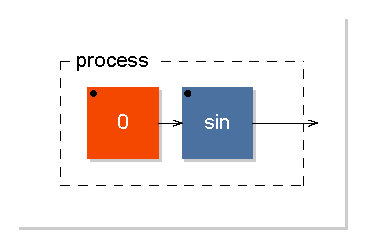
\includegraphics[]{CAPITOLI/0700/CODES/0701-seno-svg/process}
  \caption[]{Sine function. Faust Diagram.}
  \label{fdsine}
\end{figure}

\lstinputlisting{CAPITOLI/0700/CODES/0701-seno.dsp}

Questi sono i primi 5 campioni prodotti dalla formula $sin(0)$:

\lstinputlisting{CAPITOLI/0700/CODES/0701-seno.txt}

\lstinputlisting{CAPITOLI/0700/CODES/0702-senopi2.dsp}

Questi sono i primi 5 campioni prodotti dalla formula $sin(\pi/2)$:

\lstinputlisting{CAPITOLI/0700/CODES/0702-senopi2.txt}

questi i campioni

\lstinputlisting{CAPITOLI/0700/CODES/0703-senovariopi.txt}



%!TEX TS-program = xelatex
%!TEX encoding = UTF-8 Unicode
% !TEX root = ../metm.tex

\chapter{IL REPERTORIO}
\startcontents[chapters]
\printcontents[chapters]{}{1}{}

ciao\footcite[\emph{idem}]{prieberg:mexm}

Agamben \index[names]{Agamben, Giorgio}

\section{Luigi Nono}

NONO, Luigi (Venezia, 29.1.1924 – Venezia, 8.5.1990)

Nato il 29 gennaio 1924 a Venezia, primogenito di Mario Nono e Maria Manetti. Nono ebbe già nell’ambito familiare i primi stimoli per la sua formazione artistica e culturale: il nonno paterno, Luigi Nono, era un noto pittore della scuola veneziana di fine Ottocento; il prozio Urbano (fratello del pittore) uno scultore; la nonna materna, discendente dell’antica famiglia veneziana Priuli Bon, si dilettava col pianoforte e col canto spaziando dalla musica del passato alla produzione liederistica più recente (Nono ricorderà con stupore di aver rinvenuto tra i suoi spartiti una delle prime edizioni degli Italienische Lieder di Hugo Wolf accanto al Montezuma di Sacchini; Nono 1987, p. 480). La madre e il padre, di professione ingegnere, erano pianisti dilettanti che amavano cimentarsi con brani di repertorio (tra questi, il Boris Godunov di Modest Musorsgkij, spesso ricordato tra i primi ascolti nella sua fanciullezza; ibid.). Frequentatori assidui del Teatro La Fenice e di varie rassegne concertistiche, Mario e Maria Nono erano inseriti nei circoli culturali e musicali della migliore società veneziana. Grazie alla fornita discoteca del padre, Nono poté conoscere presto la musica di Beethoven, Wagner, Mahler nelle prime incisioni di direttori quali Toscanini o Mengelberg. Di non minore importanza furono le prime erratiche letture condotte sui libri della imponente biblioteca paterna (oggi in parte conservati nel lascito del compositore), dalle prime traduzioni italiane di poeti e scrittori russi, ai romanzieri americani pubblicati all’epoca da Einaudi, a Pavese, Gogol’, Rilke e vari altri autori che riaffioreranno nel corso degli anni tra le selezioni testuali delle proprie opere. In questa sfaccettata e privilegiata realtà domestica è possibile ravvisare l’origine di quella che diventerà una cifra caratteristica dell’universo artistico noniano, proiettato verso un’idea (e una pratica) della musica intesa come un’arte senza frontiere che può trovare ispirazione e fondamento in varie manifestazioni artistiche e scientifiche (pittura, architettura, letteratura, poesia, filosofia ecc.) delle diverse epoche storiche.

Intorno ai dodici anni Nono intraprese lo studio del pianoforte con una docente privata amica della madre (la signora Alessandri) e, fin da ragazzo, cominciò ad assistere agli spettacoli della Fenice e del Festival internazionale di musica contemporanea della Biennale di Venezia. Svolse i suoi studi presso il Ginnasio-Liceo classico «Marco Polo» di Venezia dove conseguì la maturità nel 1942. Nello stesso anno, per assecondare i desideri del padre, preoccupato delle incertezze della professione musicale, Nono si iscrisse alla Facoltà di Giurisprudenza dell’Università di Padova. Sempre nel 1942 egli conobbe il giovane pittore Emilio Vedova e intrecciò con lui un’amicizia che, rafforzatasi nel tempo anche grazie a varie collaborazioni artistiche, durò a fasi alterne fino alla morte del compositore.

La formazione scolastica e musicale di Nono si svolse negli anni cruciali del secondo conflitto mondiale e dell’immediato dopoguerra, in un clima familiare e intellettuale di stampo tradizionale e borghese ma perlopiù ostile al fascismo. Per motivi di salute egli fu dispensato dal servizio militare e non partecipò attivamente né alla guerra né alle successive fasi della Resistenza. Nono privilegiò nondimeno in quegli anni il contatto con giovani socialisti veneziani e personalità dell’opposizione locale, coltivando ideali politici e culturali non allineati con il regime.

Nel 1941, all’età di 17 anni, il padre gli procurò un incontro con una delle maggiori personalità musicali del tempo, Gian Francesco Malipiero, compositore che gli «aprì tutti gli orizzonti della musica» (Nono 1961, p. 3). Per qualche anno Nono seguì come studente esterno i suoi corsi di Composizione presso il Conservatorio di musica Benedetto Marcello di Venezia; dal 1943, dopo il ritiro di Malipiero dall’insegnamento di composizione, continuò a frequentare sempre da esterno la classe di contrappunto e fuga di Raffaele Cumar (ex allievo di Malipiero e Dallapiccola), approfondendo contemporaneamente in privato lo studio del pianoforte con Gino Gorini. In un periodo segnato culturalmente da una progressiva chiusura verso le esperienze d’avanguardia sviluppatesi in Europa dagli inizi del XX secolo, gli orizzonti aperti da Malipiero riguardavano lo studio di Monteverdi e della grande tradizione rinascimentale italiana (polifonica e madrigalistica), dei trattati teorici di Zarlino, Gaffurio e Vicentino, nonché la scoperta della musica di Arnold Schönberg, Anton Webern e Béla Bartók. Per la sua indole curiosa e irrequieta, Nono non riuscì mai ad adattarsi a piani di studio imposti e, ben presto, cominciò a nutrire una vera avversione per vincoli formativi legati a programmi ministeriali reputati noiosi e spesso inutili. Dopo il conseguimento del compimento inferiore e medio di composizione – sostenuti rispettivamente nel 1947 e 1949 presso il Conservatorio «Benedetto Marcello» – egli non reputò necessario coronare la sua formazione musicale con il diploma.

Nel 1946, grazie a Malipiero, Nono entrò in contatto con il giovane compositore e direttore d’orchestra veneziano Bruno Maderna, di soli quattro anni più anziano, già noto per il suo passato di fanciullo prodigio. All’incirca nello stesso periodo conobbe inoltre Luigi Dallapiccola, tra i musicisti più stimati e punto di riferimento per molti giovani della sua generazione. Delle prove compositive portate a termine prima del fondamentale incontro con Maderna resta solo la labile traccia di un ricordo (Nono 1979-80): nel 1945, durante la frequentazione di Malipiero – e influenzato anche dai suoi lunghi discorsi sulla musica del XV e XVI secolo –, Nono compose La discesa di Cristo agli inferi, brano (in seguito smarrito) forgiato sul modello delle sacre rappresentazioni e ispirato a un linguaggio di stampo monteverdiano (ivi, p. 242). Lo stimolo per il primo decisivo mutamento di rotta, dopo circa otto anni di studi musicali reputati parziali e insufficienti, sembrerebbe esser stato fornito proprio da un parere critico di Dallapiccola sulla partitura de La discesa di Cristo agli inferi, speditagli dal giovane compositore su suggerimento di Malipiero: «capisco che lei ha qui dentro nel cuore molto da esprimere, soltanto deve studiare ancora molto per poterlo esprimere» (ibid.). Queste parole costituirono per Nono una spinta a ricominciare gli studi musicali pressoché da zero in un nuovo periodo di apprendistato con Maderna. Conclusi gli studi universitari – coronati nel 1947 da una laurea in giurisprudenza con una tesi sul concetto giuridico dell’exceptio veritatis – egli poté dedicarsi solo alla musica e indirizzare il suo apprendistato verso un sentiero di conoscenza autonomo e responsabile, condotto al di fuori di ogni istituzione scolastica o accademica. (Di questo periodo 1946-47 non sono note composizioni al di fuori di un progetto vocale su liriche tratte da L’allegria di Giuseppe Ungaretti, poeta da tempo amato e ammirato.)

L’incontro con Maderna segnò in modo indelebile lo sviluppo musicale e umano di Nono, che riconobbe fino alla fine all’amico il ruolo di primo vero e grande maestro di vita.

Durante lunghe giornate trascorse tra l’abitazione di Maderna e la Biblioteca Marciana di Venezia, Nono approfondì – insieme ad altri giovani raccolti intorno al giovane maestro (Romolo Grano, Gastone Fabris e Renzo Dall’Oglio tra questi) – lo studio della musica del XV-XVI secolo, dall’ars antiqua all’ars nova francese, dai fiamminghi alla polifonia rinascimentale italiana, in un continuo confronto tra teoria e pratica. Tra gli autori più amati e analizzati: Guillaume de Machaut, John Dunstable, Johannes Ockeghem, Josquin Desprès, Adrian Willaert, Andrea e Giovanni Gabrieli, spesso trascritti a partire dall’Odhecaton di Ottaviano Petrucci. L’analisi di questo periodo storico divenne – tra la fine degli anni Quaranta e l’inizio del decennio successivo – lo stimolo per un’indagine comparata dei vari processi compositivi nella storia: data la comprensione di una tecnica musicale, il fine era scoprirne la funzione in relazione al momento storico, ricercandone nuove possibili trasformazioni o applicazioni nella musica delle epoche successive fino alla contemporaneità. Fondamentale importanza assunse per Nono l’analisi del rapporto tra lo stato del materiale, la sua elaborazione e l’epoca di produzione: fu grazie a questa peculiare ricerca che il compositore maturò la convinzione – in seguito mai abbandonata – che il linguaggio artistico deve svilupparsi di pari passo con i grandi movimenti politici e sociali del tempo, arrivando a essere una possibilità (o un mezzo) per poter intervenire all’interno di essi. Conoscere la musica del passato divenne, nel cenacolo maderniano, un mezzo per conoscere e impegnarsi responsabilmente nel proprio presente.


Fu sempre Maderna a far scoprire a Nono il manuale di tecnica compositiva di Hindemith (Unterweisung im Tonsatz, 1a ed. 1937) e, con esso, a suggergli – prima del comune approdo alla scrittura seriale – l’esistenza di soluzioni concrete e alternative nei confronti di un linguaggio armonico in crisi ormai da decenni. Nel 1948, ancora su suggerimento di Malipiero, Nono frequentò insieme a Maderna un corso internazionale di direzione d’orchestra tenuto a Venezia da Hermann Scherchen. Questo nuovo importante incontro segnò l’inizio di un lungo sodalizio (culturale e umano) tra i due giovani compositori e l’anziano direttore che, per circa cinque anni, divenne il loro fondamentale punto di riferimento. Nono cominciò a seguire Scherchen durante i suoi concerti, a soggiornare per lunghi periodi presso di lui (a Zurigo, Rapallo, Gravesano), e a collaborare dapprima come copista, poi come autore, con la sua casa editrice Ars Viva Verlag (acquisita negli anni Cinquanta dalla B. Schott’s Söhne di Magonza). Grazie a Scherchen, attraverso le sue esecuzioni e i suoi racconti, Nono entrò idealmente in stretto contatto con le esperienze – musicali e non – vissute dal direttore in Germania fin dal 1912, dalle prime esecuzioni assolute degli amati Schönberg e Webern alla realtà sociale e culturale tedesca precedente all’avvento del nazismo. Tra il 1948 e il 1949, su impulso di Scherchen Nono compose le Due liriche greche (inedite, formate da La stella mattutina e Ai Dioscuri, su testi rispettivamente di Ione di Ceo e Alceo nella traduzione italiana di Salvatore Quasimodo), dichiaratamente ispirate ai Canti di prigionia di Dallapiccola. Sempre dall’anziano direttore ricevette ulteriori stimoli allo studio della musica di Bach, Beethoven, Schumann e, soprattutto, del metodo dodecafonico, approfondito grazie all’analisi dei differenti approcci di Schönberg, Webern e Dallapiccola.

Nel 1950, su segnalazione di Scherchen e Maderna, Nono frequentò per la prima volta gli Internationale Ferienkurse für Neue Musik di Darmstadt – corsi estivi di musica contemporanea, fondamentale punto di incontro e di confronto per i giovani musicisti della generazione postbellica – debuttando sulla scena internazionale con il suo primo brano per orchestra, le Variazioni canoniche sulla serie dell’op. 41 di Arnold Schönberg (1949-50). Diretta da Scherchen, l’opera fu accolta in modo non unanime ma, al contempo, rivelò la centralità del giovane compositore nel contesto delle problematiche e delle discussioni dell’avanguardia musicale coeva. L’esperienza di Darmstadt – luogo frequentato ininterrottamente per dieci anni (dal 1957 come docente) – costituì un momento di fondamentale importanza nella sua evoluzione artistica, umana e politica. Fu qui che Nono ebbe modo di approfondire ulteriormente la musica dodecafonica e, in particolare, quella di Schönberg; di conoscere Edgard Varèse (tra gli estimatori delle Variazioni canoniche in occasione della contrastata prima esecuzione) e approcciarsi alla sua musica visionaria che tanta importanza ebbe nelle successive evoluzioni del pensiero sonoro noniano. In questa sede egli instaurò importanti rapporti – alimentati dalla consentaneità così come dal dissenso – con vari musicisti europei ed extraeuropei tra cui Karlheinz Stockhausen, Pierre Boulez, Henri Pousseur, John Cage. Soprattutto, fu a Darmstadt che si ebbero le prime esecuzioni assolute di alcune tra le più importanti pagine degli anni Cinquanta: alle già citate Variazioni canoniche seguirono infatti Polifonica-Monodia-Ritmica (1951), l’Epitaffio per Federico García Lorca I. España en el corazón (1952), La victoire de Guernica (1954), Incontri (1955), Cori di Didone (1958) e, ancora, Composizione per orchestra n. 2: Diario Polacco ’58 (1959).

Sono, queste, le opere che rivelarono Nono come uno dei maggiori rappresentanti dell’avanguardia europea e del linguaggio seriale, insieme a Stockhausen e Boulez. Da questi stessi compositori, e dall’ambiente dei Ferienkurse, egli prese nondimeno le distanze in modo dichiarato nel 1959, allorché con la conferenza Geschichte und Gegenwart in der Musik von heute (reso in italiano come Presenza storica nella musica d’oggi) polemizzò apertamente contro alcuni rappresentati dell’avanguardia e con la cosiddetta «Scuola di Darmstadt» (espressione da lui stesso coniata, cfr. Nono 1957, p. 34), denunciandone incoerenze e aporie. Dopo anni in cui gli stimoli si erano intrecciati a costruttivi conflitti, questo intervento sancì una prima frattura con il luogo e con alcuni dei suoi rappresentanti (primo tra tutti Stockhausen). L’inconciliabilità delle posizioni riguardava tanto alcune derive iperdeterministiche dei seguaci della serialità integrale e il loro rifarsi a modelli ricavati dalle scienze naturali, quanto esperienze di segno opposto riconducibili all’alea e all’indeterminazione (Cage fu apertamente nominato come pars pro toto). Entrambe le tendenze furono additate da Nono come fuga dalla storia e sintomo di una irresponsabile volontà di evitare chiare prese di posizione nei confronti di problematiche artistiche del proprio presente. La rottura, definitiva, fu quindi sancita nel 1960 con la nuova conferenza Text – Musik – Gesang (pubblicata in italiano come Testo – musica – canto), dove la distanza dalle posizioni di Stockhausen e da un’ortodossia seriale ormai vissuta come gabbia assunse infine i toni dell’aperto attacco.

Nel 1954, in occasione della prima rappresentazione del Moses und Aron di Schönberg, Nono conobbe ad Amburgo la figlia del grande compositore austriaco, Nuria, che sposò l’anno successivo. Dal matrimonio nacquero due figlie, Silvia (1959) e Serena Bastiana (1964). Tra la fine del 1958 e gli inizi del 1960 Nono compì inoltre la sua unica (nonché atipica) esperienza di docente con Helmut Lachenmann che, per lunghi periodi, soggiornò a Venezia collaborando con Nono alla formulazione tedesca delle due menzionate conferenze tenute ai Ferienkurse di Darmstadt.

Negli stessi anni Cinquanta furono di grande importanza la scoperta o l’approfondimento delle esperienze politiche e culturali d’oltralpe, della Rivoluzione sovietica e della cultura della Repubblica di Weimar, delle avanguardie storiche russe e tedesche e delle innovazioni in campo teatrale di Vsevolod Mejerchol’d, Vladimir Majakovskij, Erwin Piscator. Sollecitazioni, queste, che vennero ad aggiungersi al parallelo entusiasmo per la rivelazione dell’insegnamento di Antonio Gramsci, del pensiero filosofico di Jean-Paul Sartre, di una produzione poetica ancorata alle problematiche del proprio tempo e rappresentata da autori quali Federico García Lorca, Pablo Neruda, Paul Éluard, Cesare Pavese, Giuseppe Ungaretti.

È soprattutto da questi scrittori che Nono seleziona i testi per le proprie opere vocali degli anni Cinquanta, decennio al cui centro campeggia uno dei suoi capolavori, Il canto sospeso (1955-56), basato su lettere di condannati a morte della Resistenza europea. Abbandonato l’uso di materiali ritmici preesistenti – proprio alle sue pagine composte tra il 1950 e il 1953 – e approfondita quella personale elaborazione della tecnica seriale già avviata in campo strumentale con Canti per 13 (1955), Nono perfezionò le proprie conquiste compositive nel campo della vocalità: con Il canto sospeso approdò a una nuova pratica basata su una peculiare tecnica di frammentazione del testo, enunciato nelle sue componenti vocaliche o fonetiche in successione tra le singole voci o simultaneamente, come blocco o aggregato sonoro.

Come testimoniano anche vari scritti teorici redatti nel corso degli anni Cinquanta, è in questo periodo che si rafforzarono in Nono le proprie idee sulla capacità comunicativa della musica e sulla necessità di poter e dover esprimere attraverso la propria arte le sfaccettate contraddizioni del proprio tempo. Gradualmente la selezione dei testi fu sempre più orientata verso temi politicamente impegnati tratti dall’attualità storico-sociale del presente o dell’immediato passato. Questo aspetto si rivelò in tutta la sua evidenza a partire dall’azione scenica Intolleranza 1960 (1960-61) – opera in cui si concretizzarono per la prima volta alcune idee su un “nuovo teatro musicale” maturate nel corso degli anni Cinquanta – e giunse al culmine nella prima metà degli anni Settanta con la seconda azione composta per le scene, Al gran sole carico d’amore (1972-74, rev. 1977).

L’esperienza teatrale di Nono si era inizialmente nutrita di un sentimento di rifiuto – comune a diversi giovani compositori dell’avanguardia post-bellica – nei confronti dei modelli operistici fin de siècle, negazione in cui si rispecchiava un aperto dissenso verso l’organizzazione della società borghese. Fin dai primi progetti drammaturgici tracciati nel corso degli anni Cinquanta – tra i quali vari soggetti mai realizzati su testi di John Steinbeck, Anna Seghers e Anna Frank –, il teatro fu inteso come un luogo in cui temi attuali avrebbero dovuto essere rappresentati con mezzi espressivi e scenotecnici altrettanto originali. La ricerca di Nono in ambito scenico si concentrò in quegli anni sulle esperienze teatrali (soprattutto non musicali) del primo ventennio del Novecento. Come era avvenuto con lo studio della musica del passato condotto sotto la guida di Maderna, anche l’approdo al teatro musicale fu edificato sulla base di un’indagine storica atta ad approfondire tutte quelle esperienze artistiche che, proprio per essere state condannate o represse da regimi diversi, apparivano come modelli ancora potenzialmente attuali. Le letture condotte da Nono nel corso degli anni Cinquanta sul tema «teatro» furono numerose e discontinue: dalle esperienze di Gropius e del Bauhaus commentate da Giulio Carlo Argan (Einaudi 1951) alla storia del teatro di Baty-Chavance (Einaudi 1951), dai libri sul teatro russo e tedesco dei primi anni del Novecento (tra cui il fondamentale testo sul teatro politico di Piscator, 1929) a volumi su e di Majakovskij, Brecht, ecc. L’analisi parallela dei suoi approfondimenti teorici e dei suoi primi progetti drammaturgici sembra suggerire che già dai primi mesi del 1952 il compositore avesse posto le basi di quella personale riflessione sulle implicazioni tecniche e sulle possibilità di una funzione politica del teatro che, nel 1960-61, condusse alla prima azione scenica, Intolleranza 1960 (su testo proprio, rielaborato dal compositore a partire da un’idea di Angelo Maria Ripellino, con passi tratti da Alleg, Brecht, Éluard, Fučik, Majakovskij, Sartre e dallo stesso Ripellino; realizzato scenicamente con la collaborazione di Josef Svoboda ed Emilio Vedova). Soprattutto a causa dei suoi contenuti politici, in occasione della sua prima messa in scena (Venezia, 1961) l’opera scatenò violente contestazioni in sala e, nel panorama musicale dell’epoca, costituì un vero evento che divise il giudizio di pubblico e critica. Pressoché ignorata nella sua prima ricezione fu invece la portata innovativa dei suoi contenuti musicali: Intolleranza 1960 si poneva infatti come un’opera spartiacque, al contempo momento di sintesi e laboratorio sperimentale in cui tecniche ormai acquisite si affiancavano a nuove procedure compositive proiettate verso il futuro. In essa convergevano tutte le maggiori conquiste tecnico-linguistiche che avevano inaugurato gli anni Sessanta. Tra queste, la nuova tecnica vocale della “linea unica” sperimentata nei brani a cappella Sarà dolce tacere e «Ha venido». Canciones para Silvia (entrambe del 1960) e, tra le conquiste più importanti in prospettiva futura, l’uso del nastro magnetico e degli strumenti di produzione elettroacustica del suono. Sempre al 1960 data infatti la prima composizione elettronica di Nono, Omaggio a Emilio Vedova, realizzata presso lo Studio di Fonologia della RAI di Milano, laboratorio elettronico dove per diciannove anni, fino al 1979, egli produsse tutte le sue opere per/con nastro magnetico. A partire da questo momento, l’esperienza elettronica divenne una costante dell’itinerario creativo di Nono, che usò il mezzo tecnologico come nuova frontiera per esprimersi artisticamente in modo sempre più libero e immediato, sperimentando di volta in volta soluzioni sonore e spaziali non ottenibili con una liuteria tradizionale e, soprattutto, non più classificabili in generi musicali codificati. Fu anche grazie all’elettronica che Nono dismise gradualmente sistemi compositivi rigidamente organizzati, quali griglie seriali e di regolazione statistica dei parametri musicali (proprie alle composizioni degli anni Cinquanta), privilegiando sempre più l’organizzazione degli eventi sonori in strutture locali e l’elemento intervallare in luogo di quello ritmico. Svincolata da serie e da un preordinato controllo delle altezze, la scelta degli intervalli divenne per Nono sempre più “intuitiva”, definita localmente e proiettata verso la giustapposizione o sovrapposizione di superfici di suono complesse (blocchi, fasce, linee, ecc.).

L’impegno politico, i temi di conflittualità e denuncia sociale, il rifiuto della psicologia individuale a favore dell’amplificazione collettiva del dramma – tutti elementi propri all’orizzonte testuale di Intolleranza 1960 – divennero una costante nel corso degli anni Sessanta e Settanta, nel corso dei quali il concetto di impegno acquisì per Nono il valore di «imperativo morale» (J.P. Sartre) da affiancare a quello estetico. Il rapporto tra arte e attualità divenne sempre più intrecciato e profondo: ogni brano, realizzato o solo progettato, era concepito come un mezzo per partecipare attivamente, e con i propri strumenti specifici, a un più ampio processo di trasformazione della realtà sociale.

Spogliato il termine “ideologia” dell’accezione negativa propria della concettualizzazione marxiana, Nono ricondusse questa categoria di pensiero al significato gramsciano di “idea del mondo” esaltandone le caratteristiche di “strumento di verità” e di “funzione sociale” inscindibili dal messaggio artistico. A queste funzioni l’autore collegava senza mediazione lo sviluppo di un proprio peculiare linguaggio musicale, di una tecnica compositiva intesa anche come mezzo per arrivare a una testimonianza eticamente consapevole del proprio presente. Questo bisogno di attualità coinvolgeva il doppio piano del contenuto e della forma, binomio che caratterizzò, fin dagli esordi di Nono, il rapporto tra creazione e impegno. Ne La fabbrica illuminata (1964), per esempio, una voce dal vivo interagisce con se stessa preregistrata su nastro magnetico e vari materiali sonori (rumori, voci di operai ecc.), registrati dal vivo nella fabbrica dell’Italsider di Genova Cornigliano quindi elaborati elettronicamente in Studio. La denuncia, implicita nei testi documentari rielaborati da Giuliano Scabia sulla condizione operaia, è bilanciata in chiusura da una ferma fiducia nell’amore e nel futuro, in un chiaroscuro dramma-speranza caratteristico di molte opere vocali di Nono. Impegnate in una dimensione internazionale e terzomondista sono le successive A floresta é jovem e cheja de vida (1965-66), su testi documentari curati da Giovanni Pirelli, e Y entonces comprendió (1969-70), su testi di Carlos Franqui ed Ernesto “Che” Guevara. In queste opere l’alternanza tra voci dal vivo e preregistrate è ulteriormente sperimentata ed elaborata; si radicalizzano inoltre alcuni aspetti di prassi compositiva (intimamente legati a problematiche di prassi esecutiva) determinanti nella poetica musicale noniana degli anni Settanta-Ottanta. A partire da opere come La fabbrica illuminata o A floresta é jovem e cheja de vida il processo creativo di Nono venne infatti progressivamente a definirsi sempre a più stretto contatto con interpreti specifici, selezionati per le loro peculiarità timbriche ed espressive (in questa fase si ricordano, tra gli altri, i nomi di Carla Henius, Kadigia Bove, Elena Vicini). Grazie al lavoro condotto con gli interpreti in fase compositiva, Nono cominciò a non sentire più l’esigenza di fissare in un modo unico e definitivo la sua volontà autoriale in un’edizione a stampa (come nel caso di A floresta, ricostruita ed edita post mortem nel 1998). Soggetta a variabili ambientali, di proiezione spaziale del suono in sala, microfoniche ecc., l’opera cominciò ad essere intesa come prodotto di un processo in continuo divenire, spesso lasciata allo stadio di istruzione, appunto, progetto o schizzo e definita in forma conchiusa nelle sole direttive date all’interprete (la cui memoria spesso poteva coincidere in parte o in toto con il testo dell’opera). Anche laddove edite, come nel caso di Y entonces o della successiva Como una ola de fuerza y luz (1971-72, su testo di Julio Huasi), le creazioni venivano comunque definite gradualmente grazie a un lavoro condotto anche insieme agli interpreti (vocali, strumentali o addetti alla regia del suono) e orientato sempre più verso una pratica esecutiva del tutto atipica rispetto alle consuetudini tradizionali.

Ogni scelta testuale e/o performativa operata in questi anni testimonia della incessante volontà di Nono di intendere la musica come un mezzo di lotta, politica e sociale, per arrivare a denunciare ingiustizie e assurdità del presente. Nella biografia artistica e umana di Nono, la problematica relativa al concetto di impegno è stata (ed è ancora oggi) uno degli aspetti più complessi, dibattuti e, a seconda delle letture più o meno di parte, soggetto ad equivoci. Iscritto al Partito Comunista Italiano dal 1952 (quindi dal marzo del 1975 membro del Comitato Centrale), amico di esponenti e vertici del partito o critici marxisti militanti (Luigi Pestalozza tra questi), Nono non venne mai meno a un’ideale di artista d’avanguardia engagé, e questo anche quando – nelle ultime fasi della sua vita – l’impegno e la denuncia assunsero forme meno dirette. Il periodo più fecondo sul piano politico fu quello degli anni Sessanta-Settanta, in cui spesso i dati artistici giunsero a coincidere con quelli biografici (si pensi ai vari viaggi condotti nei paesi dell’Est a partire dal 1958, nell’URSS nel 1963 e negli anni Settanta, negli USA nel 1965 e nel 1979, nei paesi dell’America Latina – dal Cile al Perù a Cuba – a partire dal 1967; e ancora al confronto con la teoria e con la prassi del marxismo internazionale, la partecipazione alle lotte operaie degli anni Sessanta e ai movimenti studenteschi del 1968 ecc.). La militanza politica – esplicitamente dichiarata nelle scelte di carattere etico, sociale e artistico – divenne in questa fase inscindibile da quella di musicista alla continua ricerca di nuove soluzioni sonore. Proprio sul doppio terreno della politicizzazione delle opere e di un uso “rivoluzionario” dell’elettronica si consumò, nel 1964, la rottura con il suo primo editore storico, l’Ars Viva Verlag (Schott), e il conseguente passaggio alla Ricordi. Nel corso degli anni Sessanta-Settanta più volte Nono ebbe a parlare della propria musica come del prodotto di un’unione tra tecnica e ideologia, affermando a chiare lettere la propria “necessità” di declinare la musica al presente: «Sicuramente una partitura può causare una rivoluzione così poco come un quadro, una poesia o un libro; ma una musica può esattamente come un quadro, una poesia o un libro dare nota dello stato desolato della società, può contribuire, può fondare consapevolezza se le sue qualità tecniche si mantengono allo stesso livello di quelle ideologiche» (Nono 1969, p. 26). Questa e simili testimonianze contenute in altri testi redatti negli anni Sessanta (quali Il musicista nella fabbrica, 1966, o il testo di presentazione per Contrappunto dialettico alla mente, 1968) si sono rivelate spesso fuorvianti in sede critica, dove si è spesso dato più peso alle «qualità ideologiche» che alla portata innovativa e al valore artistico della sua musica.

Leggendo il dato in retrospettiva, la relazione tra arte e ideologia affonda le radici nello stesso apprendistato condotto con l’amico-mentore Maderna alla fine degli anni Quaranta e costituisce una tra le premesse creative della sua opera di esordio, di quelle Variazioni canoniche sulla serie dell’op. 41 di Arnold Schönberg intese come «conseguenza dei miei primi studi dei canoni enigmatici ma […] anche una scelta ideologica» (Nono 1979-80, p. 242). Nella fase più dichiaratamente engagée dell’evoluzione di Nono, il coinvolgimento politico procurò indiscutibili impulsi alla creazione: «sempre – scrisse presentando la Composizione per orchestra n. 2 – Diario polacco ’58, composta a seguito del suo primo viaggio in Polonia – la genesi di un mio lavoro si basa su una provocazione umana: un avvenimento, una esperienza, un testo della nostra vita provoca il mio istinto e la mia conoscenza a dare la testimonianza di me musicista-uomo» (Nono 1960, p. 433), parole applicabili anche alle ultime fasi del suo percorso artistico.

Queste «provocazioni», o stimoli, sono spesso palesi e verificabili nelle scelte dei materiali e dei collaboratori. Per le fonti testuali, gli anni Sessanta-Settanta sono segnati dalla ricerca di testi tratti da autori o soggetti storici che fossero al contempo simboli di lotta, di forza, di speranza e di sacrificio per la collettività (Karl Marx, “Che” Guevara, Rosa Luxemburg, Bertolt Brecht, Fidel Castro, Tania Bunke, ecc.). Per le fonti sonore, Nono fece spesso ricorso in questi anni a suoni concreti delle realtà operaie o di rivolta, fissati nelle sue opere con/per nastro magnetico, in cui violenza umana e sonora si intrecciano talora indelebilmente (come ne La fabbrica illuminata, in A floresta o in Non consumiamo Marx, seconda parte del dittico Musica-Manifesto n. 1, 1969). Sul fronte delle collaborazioni, si pensi a quella con Piscator nel 1965, con la realizzazione delle musiche elettroniche per lo spettacolo teatrale Die Ermittlung [L’istruttoria] di Peter Weiss; al sodalizio umano e artistico che lo legò a Claudio Abbado e Maurizio Pollini, conosciuti rispettivamente nel 1965 e nel 1966, interpreti legati indissolubilmente alla genesi di alcune tra le sue pagine più importanti (“su” e “per” Pollini fu ideata la parte pianistica di Como una ola de fuerza y luz, 1971-72 e …..sofferte onde serene…, 1976, laddove Abbado sarà sul podio delle prime assolute di Come una ola, Al gran sole carico d’amore, Prometeo); si pensi ancora al lavoro con il Living Theatre nel 1966 per il nastro di A floresta o, ancora, al lavoro collettivo con il regista e lo scenografo del teatro Taganka di Mosca (Jurij Ljubimov e David Borovskij) per Al gran sole carico d’amore. Questa seconda azione scenica, dedicata alle lotte di liberazione di tutto il mondo, segnò l’acme del periodo apertamente politico di Nono: dalla Comune di Parigi alla rivoluzione russa del 1905 a quella cubana ecc., varie sommosse per la libertà furono lette da Nono attraverso il ruolo assunto al loro interno dalle donne, simbolo di speranza forza e amore. Comporre, fare e diffondere musica, diventò dichiaratamente per il compositore un momento di sintesi dialettica tra arte e vita, vista come la sola maniera per «realizzarsi compiutamente» (Nono 1963, 144). Nei concetti di impegno e responsabilità sembra riaffiorare in Nono – apertamente negli anni centrali della sua “lotta” artistica, in modo più sotterraneo negli Ottanta – l’eco dell’insegnamento di Piscator, il cui volume Das politische Theater (del 1929, edito in Italia da Einaudi nel 1960) fu una lettura determinante per Nono nei primi anni Cinquanta, allorché il compositore prendeva gradualmente coscienza del fatto che «la sintesi di arte e politica significa suprema responsabilità, significa mettere al servizio delle supreme mete umane tutti i propri mezzi e dunque anche l’arte» (Piscator, Il teatro politico, Torino 1960, p. 48).

Ma, all’interno di una parabola compositiva quasi quarantennale che lo portò dalla serialità alla musica elettronica ai live electronics, per impegno bisogna intendere anche una visione “responsabile” della ricerca implicita in ogni nuova composizione e nella messa a punto di un linguaggio innovativo la cui rivoluzione è nel risultato sonoro. In questa prospettiva va ridimensionata, o addirittura respinta, l’idea di una presunta fase “a-politica” attribuita al Nono degli anni Ottanta: l’arte vissuta come responsabilità e impegno soggettivo (che lega l’autore, l’esecutore e l’ascoltatore) è una costante che accomuna l’intero itinerario artistico del compositore e che esula da messaggi politici, palesi o latenti.

Per la comunicazione dei propri messaggi sonori, Nono percepì come profondamente inadeguati tanto i tradizionali luoghi di produzione e diffusione musicale, quanto le procedure esecutive ad essi sottesi. Nel corso degli anni Sessanta-Settanta il lavoro si proiettò sempre più verso una dimensione collettiva; le fabbriche divennero sale da concerto; la ricerca di un nuovo teatro musicale fu equiparata tout court a una condanna delle tradizionali consuetudini di ascolto e fruizione degli spettacoli. Più che le istituzioni, furono piuttosto le forme e le consuetudini sedimentate in quelle istituzioni (culturali, concertistiche, sociali) ad essere considerate superate e discusse costantemente. Lo stesso concetto di “impegno” arrivò ad essere declinato anche nell’uso dello spazio. Nei progetti e nelle opere sceniche compiute – da Intolleranza 1960 alla «tragedia dell’ascolto» Prometeo (1984, rev. 1985) – divenne sempre più radicale la volontà di abbattere la tradizionale separazione tra scena e pubblico, vista da Nono come retaggio di una rappresentazione rituale e “antidemocratica” con «i fedeli che assistono e l’officiante che celebra» (Nono 1962, p. 122). Innovativa, in questo caso, non era l’idea in sé, già largamente dibattuta e sperimentata soprattutto in campo non musicale dalle avanguardie russe, nelle sperimentazioni di Gropius o nel teatro di Piscator (laddove in campo musicale vanno quantomeno ricordati alcuni esperimenti quali Passaggio di Luciano Berio, 1962).

Innovativa è, piuttosto, la dimensione sonora e visiva che Nono intendeva proiettare in uno spazio senza barriere, fisiche o ideali, di fruizione artistica. Lo “spazio” immaginato dal compositore – raggiunto negli anni Ottanta con la trasformazione, elaborazione e proiezione in tempo reale del suono consentita dai live electronics – era inteso come un ambiente in cui i rapporti spazio-temporali potessero infrangersi in una dimensione totale sia sul piano acustico (con la moltiplicazione e spazializzazione delle sorgenti sonore), sia su quello visivo (attraverso l’eliminazione della separazione tra scena e platea).

A metà degli anni Settanta, dopo la seconda importante tappa teatrale raggiunta con Al gran sole carico d’amore, intervenne nella vita di Nono una profonda crisi creativa amplificata dal doppio lutto che, a distanza di pochi mesi, lo colpì con la morte del padre (ottobre 1975) e della madre (gennaio 1976). Pochi anni dopo quegli eventi, così Nono rievocò quel particolare momento insieme ai cambiamenti umani e artistici che ne derivarono: «Subito dopo Al gran sole è venuto il silenzio, un silenzio inesprimibile: non avevo cioè i mezzi adatti ad esprimermi. Contemporaneamente è iniziato il mio rapporto di amicizia con Massimo Cacciari che pure conoscevo dal 1965. Ho sentito una necessità di studio non solo sul mio linguaggio musicale ma anche di analisi delle mie categorie mentali e ho ripreso a comporre con …..sofferte onde serene…, un lavoro che mi ha impegnato moltissimo» (Nono 1979-80, p. 245). Alle precedenti conquiste – quali la funzione prioritaria dell’interprete nel processo creativo, il ruolo delle tecnologie, ecc. – si affiancò una nuova tensione verso un’interiorizzazione del messaggio musicale e del concetto di impegno. Le principali caratteristiche dello stile che inaugura gli anni Ottanta – resosi manifesto a partire dal quartetto d’archi Fragmente-Stille, an Diotima, 1979-80 – sono il silenzio, la pausa, la giustapposizione di frammenti in cui pianissimi al limite dell’impercettibile si alternano a esplosioni sonore, il valore strutturale dello spazio.

Sebbene questi elementi abbiano portato alcuni critici ed esegeti a parlare di una “svolta” (memorabile l’articolo che nel 1988 Massimo Mila dedicò a quest’ultima fase noniana, intitolato appunto Nono, la svolta), o di repentine discontinuità nel percorso artistico noniano, è nondimeno da rilevare che tutti questi elementi erano già presenti in nuce (e altrimenti declinati) in diverse opere degli anni Cinquanta: silenzi e sonorità sulla soglia dell’inaudibile erano per esempio in Polifonica-Monodia-Ritmica, così come i chiaroscuri dinamici e le sonorità lacerate proprie di alcune opere degli anni Ottanta erano in Due espressioni per orchestra (1953), Il canto sospeso, La terra e la compagna (1957) o nei Cori di Didone. In aperta contraddizione con interpretazioni tecniche o stilistiche che procedono per decenni, nella totalità dell’arco creativo di Nono è possibile rintracciare il filo di uno sviluppo continuo, di un’incessante elaborazione di elementi messi al servizio di un’idea sonora immaginifica, confinante talvolta con l’utopia.

I mutamenti politici e sociali, la consapevolezza della progressiva perdita di un soggetto collettivo e dell’illusorietà di una rivoluzione sociale si palesano nelle scelte testuali delle opere degli anni Ottanta, in cui risulta evidente l’influsso dell’amico filosofo Massimo Cacciari. Friedrich Hölderlin, Rainer Maria Rilke, Robert Musil, la mistica ebraica, Walter Benjamin, Edmond Jabès, Giordano Bruno, Friedrich Nietzsche, il pensiero della tragedia e della mitologia greca: questi gli autori o testi rielaborati da Cacciari per Das atmende Klarsein (1981), Quando stanno morendo. Diario polacco n. 2 (1981), Guai ai gelidi mostri (1983) e per l’atipica opera Prometeo. A questi nuovi stimoli letterari si affiancarono le nuove risorse tecniche offerte dagli strumenti di trasformazione del suono in tempo reale (live electronics), sperimentate e approfondite in Germania presso l’Experimentalstudio der Heinrich-Strobel-Stiftung di Friburgo. Nono cominciò a frequentare questo nuovo laboratorio elettronico dal 1980 a seguito del suo addio allo Studio di Fonologia della RAI, ormai tecnologicamente vetusto, sancito dopo la messa a punto di Con Luigi Dallapiccola (1979), omaggio a una delle sue guide spirituali di gioventù e prima opera in cui i suoni – dismesso l’uso di nastri magnetici – sono trasformati in tempo reale.

Il pensiero sotteso alle creazioni dell’ultimo decennio – caratterizzate da un procedere per “tentativi” o “scelte”, e dalle costanti trasformazioni degli eventi sonori in sede di esecuzione – ricorda l’immagine dello scultore leonardiano, che «nel fare la sua opera fa per forza di braccia e di percussione a consumare il marmo, od altra pietra soverchia, ch’eccede la figura che dentro a quella si rinchiude» (Leonardo, Trattato della pittura, § «Differenza tra la pittura e la scoltura»). Questo procedere per sottrazione modellando il suono in tempo reale, spesso arricchito da nuove possibilità nate come reazioni ad errori tecnici, è evidente nel cammino che conduce al Prometeo, edificato sulle tappe preliminari di diversi brani intesi come “studi”: Das atmende Klarsein, Io, frammento dal Prometeo (1981), Quando stanno morendo. Diario polacco n. 2, Guai ai gelidi mostri. Sebbene Prometeo venga annoverato tra le opere teatrali di Nono, in esso si compie un’azione di totale scarnificazione dell’elemento scenico, del tutto dismesso, o narrativo: il “teatro”, l’azione, è nel suono, inteso come entità mobile, avulso da qualsivoglia apparato visivo e drammaturgicamente proiettato in uno spazio risonante edificato anche grazie alla struttura di legno in forma di “arca”, espressamente concepita da Renzo Piano per lo spazio della chiesa veneziana di S. Lorenzo (che ne ospitò la prima esecuzione assoluta nel 1984). Idealmente, il Prometeo può essere visto come l’approdo dei tentativi teatrali intrapresi all’indomani di Intolleranza 1960, proiettati verso un orizzonte sonoro in cui la vista lascia gradualmente il campo al puro ascolto. Sul piano dei contenuti testuali l’opera mirava invece non a una rilettura mitologica della figura di Prometeo quanto all’affermazione della sua portata “rivoluzionaria”, vista nella sua incessante ricerca di nuovi ordini che sovvertissero i precedenti: «in una parola, [del]la continuità prometeica senza fine» (Nono 1987, p. 559).

La ricerca di realtà sonore inaudite, tali da provocare non solo una differente maniera di “vivere” il suono (da parte di interpreti e fruitori) ma da richiedere anche diverse configurazioni degli spazi da concerto, è alla base dell’ultima produzione di Nono che, lontana dall’essere apolitica o disimpegnata, proietta l’ideale di un’arte tanto umana quanto impegnata nelle sfere interiori dell’“indicibile” (temi tra i più cari all’ultimo Nono, insieme a quello dell’“utopia”). All’indomani del Prometeo, conclusasi la collaborazione con Cacciari e tra soggiorni in Germania sempre più frequenti, Nono scrisse le sue opere orchestrali più visionarie: A Carlo Scarpa architetto, ai suoi infiniti possibili (1984), per orchestra a microintervalli; Caminantes… Ayacucho (1986-87) e «No hay caminos. Hay que caminar»… Andrei Tarkowskij (1987). Queste pagine per grande organico furono affiancate da brani con organico ridotto e trattamento del suono live electronics – tra queste i due omaggi a Boulez e Cacciari, A Pierre, dell’azzurro silenzio, inquietum (1985) e Risonanze erranti. Liederzyklus a Massimo Cacciari (1986) – e da brani solistici con o senza la trasformazione del suono in tempo reale: Post-Prae-Ludium per Donau (1988), La lontananza nostalgica utopica futura. Madrigale per più «caminantes» con Gidon Kremer (1988-89), scritta “sul” grande violinista citato nel titolo, e «Hay que caminar» sognando (1989), brano che chiude il catalogo noniano. Ciascuna di queste opere venne realizzata pressoché costantemente con singoli interpreti di fiducia – Roberto Fabbriciani, Ciro Scarponi, Giancarlo Schiaffini, Susanne Otto, Stefano Scodanibbio, Hans Peter Haller ecc. – spesso vicini al compositore anche nelle fasi preparatorie dell’opera in lunghe sedute di lavoro e studio presso il laboratorio elettronico di Friburgo, depositari di una volontà d’autore sempre più refrattaria ai limiti e margini di una scrittura musicale difficilmente codificabile in modo tradizionale.

Nei suoi ultimi anni di vita Nono intensificò i suoi rapporti con la Germania vivendone dall’interno le fasi che precedettero la caduta del Muro di Berlino. Altri viaggi decisivi per la genesi di alcune opere furono condotti in Spagna; fu proprio a Toledo, nel 1985, che lesse sul muro di un convento la parafrasi di un verso di Machado – «Caminantes: no hay caminos, hay que caminar» – fonte di ispirazione per il ciclo dei Caminantes che chiude il suo catalogo. Nel 1986-87 soggiornò per un lungo periodo a Berlino grazie a una borsa del DAAD (Deutscher Akademischer Austauschdienst, servizio tedesco per lo scambio accademico). Nel 1987-88 divenne membro del prestigioso istituto di ricerca Wissenschaftskolleg zu Berlin. Nel marzo 1990 vinse il Großer Kunstpreis Berlin, importante onorificenza annualmente conferita da una delle sei sezioni dell’Akademie der Künste a personalità di spicco in campo artistico. Ormai gravemente ammalato di una disfunzione epatica, Nono si spense a Venezia due mesi dopo, l’8 maggio 1990, nella sua dimora natale alle Zattere.

(Angela Ida De Benedictis, versione ampliata della voce Luigi Nono, Dizionario Biografico degli Italiani, Treccani.it L’enciclopedia italiana, Volume 78, 2013 / © Treccani. Per gentile concessione dell’editore e dell’autrice).


%!TEX TS-program = xelatex
%!TEX encoding = UTF-8 Unicode
% !TEX root = ../metm.tex

\chapter{LE FIGURE DELLA MUSICA}
\startcontents[chapters]
\printcontents[chapters]{}{1}{}

\begin{flushright}
		\textit{We think we're writing something to amuse, but \\
            we're actually saying something we desperately need to share. \\
            The real mystery is this strange need. \\
            Why can't we just hide it and shut up? \\
            Why do we have to blab? \\
            Why do human beings need to confess? \\
            Maybe if you don't have that secret confession, \\
            you don't have a poem - don't even have a story. \\
            Don't have a writer.} \\
            - Ted Hughes\footnote{Ted Hughes, \emph{The Art of Poetry No. 71}, \emph{The Paris Review}, n. 134 - 1995\\
						Pensiamo di scrivere qualcosa per intrattenere, ma | in realtà stiamo
						dicendo qualcosa che abbiamo disperatamente bisogno di condividere. |
						Il vero mistero è questo strano bisogno. | Perché non possiamo
						semplicemente nasconderlo e stare zitti? | Perché dobbiamo spifferare? |
						Perché gli esseri umani hanno bisogno di confessare? | Forse se non
						si ha quella confessione segreta, |	non si ha una poesia - non si
						ha nemmeno una storia. | Non si ha uno scrittore.}
\end{flushright}

\section{Compositore}

\emph{Chi è compositore oggi? Una persona che viene pagata per scrivere musica?
Una che produce dischi per i quali ha decine di sostenitori? Una persona che
insegna composizione? Una che è diplomata in composizione?}

La figura del compositore di musica è, oggi, un buon argomento di discussione e
\emph{deve} esserlo in ogni ambito di studi che possa presentare orizzonti compositivi.

Composizione è tecnica. Tecnica è regole. \emph{Composizione è regole?} Indispensabile
riflessione storica su questo punto è quella di Giorgio Nottoli\index{Nottoli, Giorgio} (1997) in
\emph{a proposito di musica contemporanea} pubblicato su \emph{Fisica nella Musica}
di Alberto Frova. In quel testo Nottoli\index{Nottoli, Giorgio} compone un ragionamento sulla composizione,
sull'essere compositore investendo inevitabilemente di responsabilità anche la
controparte, il fruitore, l'essere destinatario di quella che John Cage\index{Cage, John} definisce
\emph{lettera ad uno sconosciuto}: la composizone di un brano musicale.

Il testo si articola attorno ad un centro logico formato dal triangolo
\emph{regola-libertà-processo} che racchiude e protegge il cuore della composizione:
l'\emph{idea musicale}. Senza \emph{idea}, non c'è processo, né regole né
libertà d'azione. L'artista, il compositore, manipola l'\emph{idea} attraverso
questi tre canali d'intervento e ne ricava la sua \emph{composizione}.

La parabola narrativa usata da Nottoli\index{Nottoli, Giorgio} nell'articolo conduce al ruolo del fruitore,
ai sui diritti, ma anche ai suoi doveri (che dal 1997 sono purtroppo solo aumentati)
di studio, documentazione, discussione, per avvalersi di quegli strumenti culturali di analisi e
comprensione di un brano di musica d'oggi. Oggi. Perché il vero dramma
dell'essere compositori di musica oggi o, come scrive Nottoli\index{Nottoli, Giorgio}, compositori di
\emph{musica d'arte contemporanea}, è proprio quello della consapevolezza
dell'assenza di interlocutori o, più didascalicamente, di pubblico.

Se si vuole comprendere il \emph{messaggio codificato} insito in una musica e
si riconosce di non avere i requisiti minimi per la decodifica, ci si deve
impegnare per apprendere e conquistare tutte quelle le chiavi di accesso
attraverso le quali individuare i \emph{parametri} compositivi.
I \emph{come} ed i \emph{cosa} che collegano il fruitore all'ascolto, al
contesto storico del brano ed al senso che esso custidisce. Il
rapporto tra composizione e fruizione è quindi un rapporto alla pari, il
compositore e l'ascoltatore si servono di mezzi culturali condivisi per comprendersi.
Sempre che l'ascolto sia il fine ultimo, che si consideri nella musica la funzione
sociale di portare senso nell'ascolto stesso, dal quale si può anche dover
apprendere quindi, che ci stanno mancando chiavi di lettura, che bisogna studiare per
poi riascoltare.

I \emph{parametri} su cui opera il compositore d'oggi sono piuttosto sconosciuti
al fruitore d'oggi, ma come fa notare John Cage\index{Cage, John}, erano lontani anche dall'armonia
e dal carattere intervallare del contrappunto e della musica
dodecafonica\footnote{1948 - John Cage\index{Cage, John}, \emph{Confessioni di un compositore}}.
Entrambi i compositori fanno riferimento ai parametri fisici del suono, alle loro
relative sensazioni percettive, evidenziando quanto la musica sia inevitabilmente
condizionata dalla funzione che le releghiamo, una cornice in grado di oscurarne
il contenuto artistico ed ogni parametro codificato, in grado di portare in evidenza l'ormai sola ed unica
figura comprensibile e prodominante, nella cultura occidentale, della linea melodica.
Il problema culturale può essere affrontato partendo da infiniti spunti,
ma non è questo il luogo di una riflessione socio-antropologica. Potremmo
però soffermarci su alcune parole di John Cage\index{Cage, John} del 1948:

\begin{quote}
  La prima cosa che si nota a New York è la quantità incredibile di eventi. A
  Seattle, ricordo, c'era una mostra di pittura moderna che durava un mese ed
  era la sola; noi ci andavamo spesso, riflettevamo, ne parlavamo, la sentivamo
  sul serio. Suonavamo musica e ci rimaneva anche il tempo per qualche passatempo.
  Nulla di simile a New York. Ci sono talmente tanti concerti di musica, mostre
  di pittura, feste, eventi teatrali, chiamate telefoniche, una tale sequela di attività,
  che c'è da meravigliarsi come qualcuno riesca a mantenere la testa a posto\footnote{1948 -
	John Cage\index{Cage, John}, \emph{Confessioni di un compositore}}.
\end{quote}

% necessità e bisogno, fagioli.

Come qualcuno riesca ancora ad avere necessità di ascoltare. Di pensare. Vorrei
fare un ultimo ragionamento attorno alla composizione. Vorrei darle una
visione più complessa e tridimensionale.

Durante una conferenza di Michelangelo Lupone\index{Lupone, Michelangelo} a
Salerno nel 2016 lo sentii parlare per la prima volta del suo triangolo magico
di relazioni, quello composto da \emph{progetto-strumento-opera}. La visione
poetica di Lupone\index{Lupone, Michelangelo} rappresenta quanto di più monolitico prodotto negli ultimi
decenni: un legame tra tecnologia, suono, oggetto che lo evoca, spazio acustico, spazio
architettonico, percezione acustica, percezione visiva e percezione tattile.
La speculazione e la ricerca sullo strumento, sul mezzo, non è certo una novità
nel comporre musica. La sperimentazione e la ricerca sono però atteggiamenti che hanno
beneficiato enormemente degli impulsi nervosi e nevrotici che la musica elettronica
ha dato fin dai primi gemiti prodotti con le macchine. Il pensiero elettronico, o
elettroacustico, ha cambiato in maniera irrevocabile l'approccio alla composizone.
Si è insinuato nelle tecniche per cambiarle per sempre.

Dopo aver ascoltato il \emph{Prometeo} (1984) di Luigi Nono\index{Nono, Luigi} a Parma (2017), mi sono chiesto a lungo
dove fosse finita quella poetica,
quel modo di vedere e sentire la musica. La mia indagine si è conclusa circa un anno dopo, quando ho
analizzato \emph{Canto di madre} (1998) di Michelangelo Lupone\index{Lupone, Michelangelo}.
Quella poetica, con le giuste proporzioni socio-economiche,
non è mai sparita, ed è custodita proprio in questi triangoli di prassi compositiva: \emph{progetto-strumento-opera}
e \emph{regola-libertà-processo}. L'idea musicale e la poetica musicale contemporanea
sono vive, pulsano di ricerca, passione e desiderio di condivisione di un pensiero
racchiuso tra queste sei coordinate spaziali \emph{regola-libertà-processo-progetto-strumento-opera}.
Sei. In geometria tridimensionale con sei lati si descrive il primo solido regolare. Uno scrigno.
Una struttura ossea attorno ad un cuore pulsante.

\begin{quote}
  Dopo diciotto mesi di studio della filosofia e del misticismo orientali e del
  cristianesimo medievale, iniziai a leggere gli scritti di Jung sull'integrazione
  della personalità. Ci sono due componenti principali in ogni personalità:
  la mente cosciente e quella inconscia, e queste, nella maggior parte di noi,
  sono divise e disperse in infiniti modi e direzioni. La funzione della musica,
  come quella di ogni altra salutare attività, è quella di aiutare a riportare a
  una unità queste parti separate. La musica fa questo fornendo un momento in cui,
  essendo smarrita la consapevolezza dello spazio e del tempo, viene integrata la
  molteplicità degli elementi che costituisce un individuo ed egli è uno. Questo succede
  soltanto se, di fronte alla musica, non ci si lascia andare alla prigrizia e alla distrazione.
  Le occupazioni di molte persone oggi non solo non sono salutari, ma rendono malati coloro
  che le praticano, perché sviluppano una parte dell'individuo a detrimento dell'altra.
  Il malessere che ne risulta è in primo luogo psicologico, per questo si prendono periodi
  di vancanza dal lavoro per rimuoverlo. Ma poi la malattia attacca tutto l'organismo.
  [\ldots] Se uno fa musica, come direbbero in Oriente, \emph{disinteressatamente}, cioè
  senza alcun interesse per i soldi o la fama, ma soltanto per l'amore di farlo,
  compie un'attività di integrazione e troverà momenti nella vita che sono completi e
  appaganti. A volte è la composizione a farlo, a volte è suonare uno strumento, a
  volte è solo l'ascolto\footnote{1948 - John Cage\index{Cage, John}, \emph{Confessioni di un compositore}}.
\end{quote}

Il pensiero di Cage è lontano decenni da noi, dal nostro rapporto con l'arte e la
musica. Abbiamo una vaga idea di dove siamo ora con l'ascolto e con l'attenzione? La musica
elettronica ha lungamente trainato il pensiero musicale prima di essere messa a servizio,
funzionale alla macchina mercantile.

\begin{quote}
  La musica elettronica fu possibile solo quando la musica cessò di esistere come
  linguaggio costituito e come metafora linguistica, da quando il compositore
  cominciò a inventare e a elaborare "fonemi" (nel senso già indicato da Debussy, per esempio)
  e non a manipolare "parole" belle e fatte; da quando potè riprendere coscienza
  del fatto che le note non sono il materiale della musica ma solamente segni convenzionali
  dietro i quali si celano fenomeni concreti e che agire musicalmente significa organizzare la
  percezione e non le note\footnote{1961 - Luciano Berio\index{Berio, Luciano}, \emph{Musica sperimentale e musica radicale.}}.
\end{quote}

Non lo erano le note, il materiale della musica, non lo devono essere nemmeno i
nuovi mezzi di produzione sonora.

\begin{quote}
  Se questi ultimi hanno qualcosa da insegnare [al] di là della loro pratica utilizzazione,
  è proprio la incostituzionalità e la deficienza di un'assunzione "linguistica" della musica
  (senza per questo voler negare all'opera compiuta una sua struttra pensabile e
	riferibile).\footnote{1961 - Luciano Berio\index{Berio, Luciano}, \emph{Musica sperimentale e musica radicale.}}.
\end{quote}

Mi servo delle parole di Berio\index{Berio, Luciano} per cercare di capire in che momento questa coscienza
è involuta trascinandosi dietro la tecnologia, la scienza del suono. Qual è stato
il traino involutivo che ha trasformato un'opportunità di liberazione e consapevolezza
in un materiale linguistico.

\begin{quote}
  "Prima" dell'opera compiuta non esistono perciò materiali, ma situazioni di fatto
  naturali e culturali che noi assumiamo e trasformiamo di continuo, sulla base delle
  quali noi giungiamo a stabilire un certo campo d'azione possibile. Che io poi dia
  corpo alla mia opera valendomi di un'orchestra, di un pianoforte, di suoni
  prodotti elettricamente, registrati al microfono o tutte queste cose assieme,
  significherà semplicemente che l'idea di quell'opera implicava quei mezzi
  e non altri, e che mi verranno posti determianti problemi e determinate
  soluzioni piuttosto che altre: quello del compositore è pure sempre un
	mestiere!\footnote{1961 - Luciano Berio\index{Berio, Luciano}, \emph{Musica sperimentale e musica radicale.}}.
\end{quote}

Il pensiero di Berio\index{Berio, Luciano} completa il quadro poietico e poetico, fa da sfondo, è la storia
del pensiero emerso con Nottoli\index{Nottoli, Giorgio} e Lupone\index{Lupone, Michelangelo}, si concentra sull'idea musicale, sugli
inevitabili rapporti tra opera, struttura, progetto, mezzi, e quindi strumenti, un
campo d'azione con le sue regole e le sue libertà soggettive. È di nuovo un forte
legame con la storia alla base del quale si può ripartire con un'idea di \emph{scuola}
di composizione.

\begin{quote}
  Quello che più conta, infine, è di saper educare noi stessi e gli altri a
  considerare l'arte come una formazione, non come un
	funzionamento\footnote{1961 - Luciano Berio\index{Berio, Luciano}, \emph{Musica sperimentale e musica radicale.}}.
\end{quote}

%------------------------- APPROFONDIMENTO
		\begin{tabular}{L{.969\textwidth}}%
		\toprule
			\textbf{Composizione}\\
		\midrule
			dal lat. \emph{compositio -onis}, der. di \emph{componere} comporre.

			\begin{compactitem}
        \item L’atto, l’operazione, il lavoro del comporre, cioè del mettere
          ordinatamente e organicamente insieme; e anche il risultato di tale
          operazione: \emph{iniziare la c. di un mosaico; attendere alla c. di
          un poema, di una sinfonia; tinta ottenuta con una sapiente c. di colori;
          l’armonia risulta dalla c. di varî suoni}. Usato assol., nelle frasi
          studiare c., insegnare c. e sim., s’intende l’arte del comporre musica
          e la sua didattica. Nelle arti figurative e in fotografia, il modo in
          cui sono distribuiti, organizzati e messi in luce i vari elementi
          figurativi, con riguardo soprattutto all’unità stilistica; in
          architettura, il modo e il criterio con cui sono disposte e organizzate
          le diverse parti di un edificio o di più edifici tra loro
          (rispettivam., \emph{c. architettonica} e \emph{c. urbanistica}).
        \item L’insieme degli elementi di cui una cosa è composta, con riguardo
          alla natura o alla qualità di ciascuno o al loro reciproco rapporto:
          \emph{non si conosce ancora la c. della giuria; la c. dello sciroppo è
          descritta sull’etichetta}. Con sign. più specifico, \emph{c. chimica},
          il nome degli elementi e i rapporti in cui essi entrano a far parte
          della molecola di un composto: \emph{la c. dell’acido solforico}.
        \item La cosa stessa composta: \emph{questa bibita è una c. di diversi ingredienti;}
          spec. di opera d’arte: \emph{c. musicale, c. per canto e pianoforte;
          c. drammatica, poetica; mi ha letto una sua breve c. in versi;
          ha dipinto una c. allegorica;} meno com., lavoro scritto assegnato
          agli studenti, componimento.\footnote{\url{http://www.treccani.it/vocabolario/composizione/}}
      \end{compactitem} \\
    \bottomrule
		\end{tabular}
%------------------------- APPROFONDIMENTO

\section{Interprete}
\section{R.I.M.}
\section{Regista}


%!TEX TS-program = xelatex
%!TEX encoding = UTF-8 Unicode
% !TEX root = ../../metm.tex

\chapter{STEREOFONIA}
\startcontents[chapters]
\printcontents[chapters]{}{1}{}

\vfill\null

Il primo passo necessario verso la comprensione del concetto di \emph{Stereofonia},
per di arrivare alle tecniche ed alle tecnologie elettroacustiche che la
rendono possibile, è stabilire attraverso l'etimologia del termine, e dei
termini ad esso collegati, una base concettuale solida. \emph{Stereo}, dal greco
\emph{Stere\'os}, significa \emph{solido}. Non un numero, non una configurazione
ma un aggettivo qualitativo. Nel dizionario inglese Oxford: \emph{Solid, firm
and stable in shape. Having three dimensions}. Solido, \emph{solid}, dalla radice
latina di \emph{Solidus, Sollus}, intero.

Con la parola \emph{Stereofonia} dovremmo quindi descrivere una condizione
nella quale \emph{phon\={e}}, sempre dal greco, \emph{suono}, la \emph{voce},
arrivi all'ascoltatore solida, integra, ferma e stabile nella sua forma (sonora)
multi dimensionale, intera.

%\clearpage

Indispensabile alla comprensione è anche la descrizione del concetto di \emph{mono}, nomignolo di
\emph{monofonico}, espresso nel legame tra \emph{monos} e \emph{phon\={e}}: una voce,
\emph{one voice}, \emph{alone}, sola. La stessa parola usata nella descrizione
del canto gregoriano ad una voce, successivamente evolutasi nella \emph{polifonia}
(dal greco \emph{poluph\={o}nia}, da \emph{polu}, molte e \emph{phon\={e}},
voci). Quindi la dicotomia, se proprio deve essercene una, tra monofonia e
stereofonia semplicemente non esiste. L'estensione del concetto di monofonia,
nel suo eventuale opposto, è polifonia. La stereofonia è semplicemente un
concetto altro.

Con la parola stereofonia dovremmo descrivere anche la condizione in base alla
quale il suono arrivi \emph{solido} all'ascoltatore, \emph{intero, fermo e
stabile} nella sua forma sonora multidimensionale originaria, attraverso
la riproduzione elettroacustica, attraverso la trasmissione e la diffusione mediante
altoparlanti, con un numero qualsiasi, o necessario, di canali. In questo caso,
facendo riferimento alla definizione dell'aggettivo \emph{stereofònico}, ci
si apre alle tecniche ed alle tecnologie che hanno reso possibile la
trasmissione, la riproduzione e la diffusione del suono in stereofonia.
Un aggettivo che dovrebbe essere usato con cautela, nella circostanza in cui la
riproduzione dei suoni avvenga in modo
che l’ascoltatore abbia l’impressione di trovarsi nello spazio sonoro originale o,
nel caso non ve ne sia, per sorgenti di natura non acustica, che restituiscano
informazioni tali da descrivere una correlazione al sistema percettivo, simile a
quella suggerita da sorgenti acustiche.

Condizioni di ascolto stereofoniche, dal latino \emph{auscultare}, prestare
attenzione a qualcosa in quanto oggetto o motivo di informazione, nel caso specifico,
informazioni di stereofonia.

\vfill\null

%------------------------- APPROFONDIMENTO
%\begin{figure}[th]
\begin{table}[ht]
\footnotesize
\begin{tabular}{L{.969\textwidth}}%
\toprule
	\textbf{Alan Dower Blumlein}\\
\midrule
Nato il 29 giugno 1903 a Londra, Deceduto il 7 giugno 1942 a Herefordshire,
Inghilterra, fu ingegnere elettronico presso EMI, per la quale pubblicò brevetti
per le sue numerose invenzioni nel campo delle telecomunicazioni soprattutto in
relazione alle tecnologie di registrazione, trasmissione e diffusione del suono.
Ottiene, nella sua breve carriera, 128 brevetti, motivo per cui è considerato
uno dei più importanti ingegneri e inventori del suo tempo. Morì durante la
seconda guerra mondiale all'età di 38 anni, durante un test militare segreto del
sistema radar H2S allora in fase di sviluppo, a bordo del bombardiere Halifax
su cui stava volando. Tra le numerose invenzioni legate al nome di Blumlein
quelle legate alla Stereofonia stravolsero completamente il mondo della
fruizione pubblica del suono. Le sue prime note sull'argomento risalgono al 25
settembre 1931 e il suo brevetto aveva il titolo “Miglioramenti ai, ed in
relazione ai, sistemi di trasmissione, registrazione e riproduzione del suono”.
La domanda di brevetto fu del 14 dicembre 1931 ed la concessione fu dell
14 giugno 1933, brevetto britannico numero 394.325.\\
\bottomrule
\end{tabular}
\end{table}
%\end{figure}
%------------------------- APPROFONDIMENTO

%%%%%%%%%%%%%%%%%%%%%%%%%%%%%%%%%%%%%%%%%%%%%%%%%%%%%%%%%%%%%%%%%%%%%% LE RADICI
%%%%%%%%%%%%%%%%%%%%%%%%%%%%%%%%%%%%%%%%%%%%%%%%%%%%%%%%%%%%%%%%%%%%%%%%%%%%%%%%
\section{Radici}

L'\emph{International Exposition of Electricity}, tenutasi nel 1881, ha mostrato
cose come l'illuminazione elettrica con Edison e altri che presentano le loro
lampadine a incandescenza.

Uno dei reperti era un "telefono stereo". Nel 1881 Alexander Graham Bell aveva un modello funzionante del suo telefono, ma era il francese Clément Ader la cui invenzione fu esposta [2]. Forse la ragione è stata la decisione del governo britannico di non sprecare denaro pubblico sponsorizzando l'evento. Ogni sera veniva suonata musica alla Grande Opera e la gente poteva ascoltare per alcuni minuti al telefono a circa due chilometri di distanza al Palais de Industrie, dove si teneva l'esposizione. Una serie di dieci microfoni al carbonio è stata posizionata lungo la larghezza del palco. Ciascuno di questi era collegato a otto stazioni di ascolto all'estremità opposta. Si potrebbe pensare che, dato che il telefono era ancora agli inizi, per i membri del pubblico semplicemente ascoltare la performance sarebbe stato sufficiente, ma Ader ha aggiunto l'esperienza di "stereo". Ogni persona che ascoltava aveva due auricolari, uno per ciascun orecchio. Ogni auricolare ha presentato la performance da una posizione separata sul palco (ad es. Microfoni 1 e 6, 2 e 7, e così via) consentendo così all'ascoltatore di valutare la posizione laterale dell'esecutore. Fortunatamente, l'esperimento ebbe successo e nacque "stereo". Diversi anni dopo l'Expo di Parigi del 1881, l'invenzione fu usata commercialmente in Francia e in Inghilterra. Il telefono e la rete richiesta furono sviluppati, così come la distribuzione di energia elettrica, ma il prossimo traguardo per lo stereo non sarebbe arrivato fino a 50 anni dopo.

La percezione dei caratteri spazio-temporali dei suoni, in particolare della
loro direzione di provenienza e della loro relazione con lo spazio che
attraversano, definiscono i tratti essenziali della stereofonia, in relazione
all'udito, in virtù dell’audizione biauricolare (o binaurale). Come sottolineato
nell'enciclopedia Treccani, tra le varie definizioni di stereofonia \emph{il
termine è inoltre usato per indicare la parte dell’acustica fisiologica
che si occupa di tale fenomeno}. L'ascolto biauricolare del sistema uditivo
conferisce alla percezione umana il potere localizzatore, cioè la capacità,
dovuta al lavoro congiunto dei due sistemi auricolari separati ed al sistema
nervoso centrale, di determinare la direzione di provenienza di un suono. In tal
senso, esiste in acustica fisiologica la definizione di monofonia in qualità di
condizione anomala del sistema percettivo, caratterizzata dalla mancanza degli
elementi necessari a individuare i caratteri spaziali dei suoni stessi, come per
esempio quella ottenuta con un solo orecchio.

L'ultimo esercizio linguistico è legato alla definizione dell'aggettivo
\emph{stereofònico} e ci permette di aprire il termine alle tecniche ed alle
tecnologie che hanno reso possibile la trasmissione, la riproduzione,
e la diffusione della stereofonia. \emph{Stereofònico}, quindi, che si riferisce
alla stereofonia, alla percezione della stereofonia, alla descrizione delle
tecniche di registrazione e riproduzione in grado di operare stereofonia. Un
aggettivo che dovrebbe essere usato solo nella
descrizione di tecniche di registrazione e di diffusione sonora atte alla
riproduzione dei suoni in modo che l’ascoltatore abbia l’impressione di trovarsi
nello spazio sonoro originale, dai quali ne deriva una musica stereofonica ed
una discografia stereofonica in grado di grarantire l’ambiente sonoro originale,
solido e tridimensionale attraverso l’effetto stereofonico.

\begin{quotation}
An observer in the room is listening with two ears, so that echoes reach him
with the directional significance which he associates with the music performed
in such room. He therefore discount these echoes and psychologically focuses
his attention on the source of the sound. When the music is reproduced through
a single channel the echoes arrive from the same direction as the direct sound
so that confusion results. [\ldots] Human ability to determine the direction
from which sound arrives is due to binaural hearing, the brain being able to
detect differences between sound received by the two ears from the same source
and thus to determine angular directions from which various sounds
arrive\footnote{Un osservatore nella stanza sta ascoltando con due orecchie, in
modo che gli echi lo raggiungano con il significato direzionale che associa alla
musica eseguita in quella stanza. Pertanto, non tiene conto di questi echi e
focalizza psicologicamente la sua attenzione sulla fonte del suono. Quando la
musica viene riprodotta attraverso un singolo canale, gli echi arrivano dalla
stessa direzione del suono diretto, in modo da creare confusione. [...] La
capacità umana di determinare la direzione da cui proviene il suono è dovuta
all'udito binaurale, il cervello è in grado di rilevare le differenze tra il
suono ricevuto dalle due orecchie dalla stessa fonte e quindi di determinare le
direzioni angolari da cui provengono i vari suoni.}. [\cite{ab58}]
\end{quotation}

Con queste parole Blumlein nel 1931 descrive i fondamenti di almeno due grandi
argomenti: quali erano le conoscenze  dell'epoca su come percepiamo i suoni
acustici e come abbiamo riprodotto i suoni fino a quel momento.

La binauralità dell'ascolto umano è la prima affermazione di Blumlein:
“\emph{un osservatore nella stanza sta ascoltando con due orecchie}”. Come
questa condizione di ascolto si evolva nel tempo è la peculiarità della
stereofonia.

% Non è correlato al numero di fonti, nemmeno al numero di microfoni
% e altoparlanti necessari per riprodurre tale condizione. La tecnica e lo scopo
% della tecnica prescelta si concentreranno per risolvere più argomenti possibili
% per soddisfare tale condizione.

%%%%%%%%%%%%%%%%%%%%%%%%%%%%%%%%%%%%%%%%%%%%%%%%%%%%%%%%%%%%%%%%%%%%%%%%%%%%%%%%%%%%%%%%%%%%%%%%%% dalle esposizioni
Dovremmo indicare quindi qualitativamente una condizione di ascolto, dal latino
\emph{auscultare}, prestare attenzione a qualcosa in quanto oggetto o motivo di informazione, con specifiche caratteristiche di solidità spaziale, dimensionalità osservabili nella forma sonora riconoscibile, informativa.

\emph{Una voce in una piccola stanza riverberante è una condizione d'ascolto che
rispetti queste qualità?}

Prima di approfondire questioni di propagazione e percezione del suono, val la pena
dedicare un tempo alla letteratura specializzata.

\begin{quote}
When recording music considerable trouble is experienced with the unpleasant
effects produced by echoes wich in the normal way would not be noticed by anyone
listening in the room in which the performance is taking place. An observer in
the room is listening with two ears, so that echoes reach him with the directional
significance which he associates with the music performed in such room. He,
therefore, discounts these echoes and psychologically focuses his attention on
the source of the sound\footnote{Quando si registra musica acustica, si riscontrano
notevoli problemi a causa degli effetti indesiderati prodotti dalle riflessioni
acustiche dell'ambiente, che nell'ascolto normale non vengono notati dagli
ascoltatori nella stanza in cui si svolge l'esibizione. L'ascoltatore, nella stanza,
ascolta attraverso le due orecchie, le riflessioni lo raggiungano con il significato direzionale che associa alla musica eseguita in quella stanza.
Pertanto, elimina dal messaggio le informazioni delle riflessioni e focalizza
psicologicamente la sua attenzione sulla sorgente sonora.}.
\end{quote}

Richiesta di brevetto numero 394325 del 14 dicembre 1931, accettazione del 14
giugno 1933. Alan Dower Blumlein.

La risposta alla domanda \emph{Una voce in una piccola stanza riverberante è una
condizione d'ascolto che rispetti queste qualità?} è, in funzione di quanto
appena letto, chiaramente affermativa.

Anche con un solo oggetto sonoro, una sola voce, in una piccola stanza, siamo in
presenza di un fenomeno acustico stereofonico. Almeno così dice Blumlein, papà
della stereofonia, nel brevetto in cui ne rende i concetti fondamentali, solidi,
stabili nel tempo e nello spazio delle parole, nel brevetto tecnologico che stabilisce
il \emph{point break} dell'elettroacustica, per il resto dell'umanità.


%%%%%%%%%%%%%%%%%%%%%%%%%%%%%%%%%%%%%%%%%%%%%%%%%%%%%%%%%%%%%%%%%%% SECTION FOUR
%%%%%%%%%%%%%%%%%%%%%%%%%%%%%%%%%%%%%%%%%%%%%%%%%%%%%%%%%%%%%%%%%%%%%%%%%%%%%%%%
\section{Ramificazioni}

Con la profonda conoscenza del significato del tempo trascorso tra noi e Blumlein,
si può ora esporre il significato dello strumento altoparlante in maniera più
dettagliata e consapevole. Per l'era
Blumlein, l'altoparlante era lo strumento futuro per un tempo presente migliore.
Il suono riprodotto, alla sua giovane età, era pura magia. Oggi sappiamo bene
quanto siamo insoddisfatti della riproduzione degli altoparlanti. Quando il
primo \emph{iPhone} è stata l'unica cosa intelligente sul pianeta è stato fantastico,
un fantastico oggetto di creazione. Oggi con lo stesso oggetto non faremmo
nemmeno una foto. Ascoltare un assolo di violino riprodotto dal miglior
altoparlante sul mercato non rappresenta la stessa esperienza della performance reale.
L'artificio non è legato alla stereofonia e all'abilità tecnica, è parte integrante del
limite della tecnologia di riproduzione che siamo in grado di realizzare.

\emph{Una voce in una piccola stanza riverberante è una condizione d'ascolto
stereofonica?} Abbiamo chiarito, con l'ausilio delle parole di Blumlein, che lo è.

\begin{quotation}
When recording music considerable trouble is experienced with the unpleasant
effects produced by echoes wich in the normal way would not be noticed by anyone
listening in the room in which the performance is taking place. [\ldots]
When the music is reproduced through
a single channel the echoes arrive from the same direction as the direct sound
so that confusion results.
\end{quotation}

Sostituendo la voce umana con la sua registrazione riprodotta da un singolo
altoparlante perdiamo, come descritto da Blumlein, la capacità del sistema
orecchie-cervello di decifrare la relazione originaria tra suono e ambiente.
Non è più lo stesso ascolto stereofonico. Diventa un altro aslcolto, una nuova
condizione di ascolto. Il numero di fonti è lo stesso. Entrambi nel loro
linguaggio monofonico producono una diversa condizione di ascolto.

Nel 1992 Michael Gerzon disegna una rappresentazione schematica delle diverse
posizioni degli altoparlanti per stereo multispeaker, da una a cinque:

\begin{quotation}
\ldots we show the loudspeaker layouts considered for frontal stage stereo
using from one (regarding mono as the trivial case of “one-loudspeaker stereo”!)
to five loudspeakers\footnote{\cite{mg92pdmsss} - mostriamo le disposizioni
degli altoparlanti considerati per lo stereo frontale partendo da uno
(considerando il mono come il banale caso dello “stereo con un solo altoparlante”!}.
\end{quotation}

Esiste una condizione di stereofonia possibile con un solo altoparlante? Ovviamente si.

Un altoparlante è in grado di suonare se stesso, il suo mondo elettrico, svincolato
dalla riproduzione di qualcosa di acustico. Un altoparlante solo, di qualsiasi tipo,
può essere messo nella condizione stereofonica di produrre un suono che non esisterebbe di esso,
con caratteristiche generali, di stereofonia e percezione binaurali assimilabili alla voce parlante.
Un rumore rosa filtrato che canta monofonicamente in una stanza è una meravigliosa condizione di stereofonia.

\subsection{Sullo strumento \emph{Altoparlante}}

L'enciclopedia britannica cataloga con una inequivocabile descrizione il termine
\emph{Loudspeaker: SOUND INSTRUMENT}. Il passaggio da altoparlante, strumento
sonoro, ad altoparlante strumento musicale, è breve, è necessario solo un musicista.

La scelta dell'altoparlante, la conoscenza del suo carattere e delle caratteristiche
tecniche è un momento necessario per quel musicista, un momento che richiede tempo.
Cambiare manualmente la frequenza di un suono sinusoidale riprodotto da un
altoparlante a tre vie, a un metro di distanza, con le orecchie alla stessa
altezza del baricentro dello strumento, è un buon modo per conoscere l'altoparlante. Il musicista scoprirà in questo modo che i
suoni prodotti dall'altoparlante cambieranno forma durante il glissato. Forse
vicino al punto di incrocio del crossover troverà alcune peculiarità, altre
strane decorrelazioni di fase ad altissima frequenza.

Scoprire e conoscoere lo strumento altoparlante e conoscere il sistema percettivo
in termini di meccanismi psico-acustici sono condizioni necessarie per
affrontare correttamente un percorso di emancipazione nei confronti dei limiti
tecnici e tecnologici nella riproduzione, produzione elettroacustica dei suoni.
Michael Gerzon, dagli anni settanta agli anni novanta, ha descritto molteplici
approcci di risoluzione dei problemi legati alla stereofonia, sempre attingendo
alle radici dell'era Blumlein, con tentativi di progettare tecnologie di
riproduzione con lo scopo di colmare il divario rispetto al regno acustico.

\begin{quotation}
The ears and brain localize sounds according to many different mechanisms. Among
the most important cues used are low-frequency interaural phase (applicable up
to around $2KHz$, but dominant below $700Hz$) and localization by
amplitude differences between the two ears, predominantly above about
$1KHz$. While other cues are also important, we have found that satisfying
both these cues, and making them mutually consistent for central listener facing
in any direction, leads to particularly robust and reliable localization
quality.\footnote{\cite{mg92pdmsss} - Le orecchie e il cervello localizzano i
suoni secondo molti meccanismi diversi. Tra i segnali più importanti utilizzati
vi sono la fase interaurale a bassa frequenza (applicabile fino a circa $2KHz$,
ma dominante al di sotto di $700Hz$) e la localizzazione mediante
differenze di ampiezza tra le due orecchie, prevalentemente al di sopra di
circa $1KHz$. Sebbene anche altri segnali siano importanti, abbiamo
scoperto che soddisfare entrambi questi segnali e renderli reciprocamente
coerenti per l'ascoltatore centrale rivolto verso qualsiasi direzione, porta
a una qualità di localizzazione particolarmente solida e affidabile.}
\end{quotation}

%%%%%%%%%%%%%%%%%%%%%%%%%%%%%%%%%%%%%%%%%%%%%%%%%%%%%%%%%%%%%%%%%%%% SUBSECTION
%%%%%%%%%%%%%%%%%%%%%%%%%%%%%%%%%%%%%%%%%%%%%%%%%%%%%%%%%%%%%%%%%%%%%%%%%%%%%%%%
\subsection{Sul concetto di \emph{PanPot}}
\label{sec:panpot}

L'oggetto \emph{panner} è rappresentato da un potenziometro di controllo
(hardware o software, in entrambi i casi a controllo analogico o digitale) che
regola la distribuzione di un segnale su più canali componenti un campo sonoro
stereo o multicanale. Ogni mixer ha un \emph{panpot} (abbreviazione di
\emph{potenziometro di panoramica}), per ciascun canale sorgente in ingresso,
che regola l'azione del \emph{panner}.

%L'ultima precisazione riguarda il movimento panoramico. La distribuzione dell'energia
%o la condizione della coppia di segnali che regola il movimento panoramico troppo
%spesso sono descritti come la possibilità di muovere gli oggetti attorno alla posizione
%dell'ascoltatore.

Generalmente il \emph{panpot} viene descritto come un pomello che permette di
muovere i suoni tra la sinistra e la destra del panorama di diffusione, il che è
parzialmente vero e potenzialmente pericoloso in termini di immaginazione
acustica.

Soffermandosi ad analizzare il fenomeno acustico di un suono prodotto da un
oggetto in movimento tra la destra e la sinistra di un campo percettivo emergono
diversi problemi.

Il primo riguarda l'\emph{effetto doppler}. Siamo seduti su una panchina al
margine di una strada che si estende infinita agli estremi della nostra vista
periferica. Un mezzo di soccorso, con la sirena accesa, si avvicina percorrendo
la strada davanti al nostro viso, da sinistra verso destra: percepiamo
una variazione in frequenza al passaggio della sirena, in funzione della
velocità. L'\emph{effetto doppler} ci descrive come nel percorso di
avvicinamento a noi la frequenza sale lentamente fino al massimo ottenuto nel
momento in cui ci raggiunge per poi diminuire rapidamente in coincidenza con
l'allontanamento.

Ora siamo dei \emph{sound designer}, siamo seduti di fronte alla nostra console
analogica e dobbiamo replicare l'effetto sopra descritto. Applicando un
movimento da sinistra a destra, azionando il \emph{panpot} su un suono di sirena
statico, registrato fermo ad un metro di distanza, pur ruotando velocemente il
potenziometro non otteniamo variazioni in frequenza. Il suono si muove tra la
sinistra e la destra del sistema d'ascolto senza produrre il movimento nello
spazio ma solamente lo spostamento della posizione relativa al nostro punto di
ascolto. Ne deriva una prima conslusione: il \emph{panpot} regola una posizione
relativa, non stabilisce criteri di movimento.

Un altro problema emergente del pensare il \emph{panning} come un movimento
scaturisce dalla relazione della sorgente con l'ambiente circostante. Che
movimento può esserci senza tenere conto del luogo in cui la sorgente sonora si
trova? Un avvocato pronuncia la sua arringa in tribunale parlando ad alta voce,
camminando, rimbalzando tra destra e sinistra. La voce si propaga nello spazio
ed è inevitabile che se ne percepisca la variazione topologica, morfologica in
relazione con le caratteristiche architettoniche: a sinistra della stanza c'è
una parete di finestre, a destra un muro in cemento. Pur non avendo velocità
sufficiente ad innescare l'effetto doppler, la sua continua variazione di
posizione corrisponde ad una continua variazione di rapporto con l'ambiente che
lo circonda, in relazione ad ogni infinto punto di ascolto all'interno della
stanza. In altre parole, quel movimento assume significati diversi relativi al
punto di ascolto.

Dovendo simulare lo stesso effetto mediante l'azione sul panpot, otterremmo la
variazione di posizione della voce nello spazio, ma non la sua relazione con lo
spazio.

\begin{figure*}[t!]
    \centering
    \begin{subfigure}[t]{0.45\textwidth}
        \centering
        \includegraphics[height=8cm]{CAPITOLI/_TIKZ/PANNING/pan-frontal}
        \caption{Sorgente con incidenza frontale.}
        \label{pan:frontal}
    \end{subfigure}%
    ~
    \begin{subfigure}[t]{0.45\textwidth}
        \centering
        \includegraphics[height=8cm]{CAPITOLI/_TIKZ/PANNING/pan-left}
        \caption{Sorgente con incidenza laterale sinistra di 30 gradi.}
        \label{pan:left}
    \end{subfigure}
    \\
    \begin{subfigure}[t]{0.9\textwidth}
        \centering
        \includegraphics[height=8cm]{CAPITOLI/_TIKZ/PANNING/pan-both}
        \caption{Due sorgenti, una con incidenza laterale sinistra di 30 gradi,
        l'altra con incidenza laterale destra di 60 gradi.}
        \label{pan:both}
    \end{subfigure}
    \caption{La rotazione del \emph{PanPot} esegue una modifica della condizione
    di ascolto dell'ascoltatore, non un movimento della sorgente. Posizionando
    le singole sorgenti ci si pone in ascolto laterale, ruotati. Nella
    sovrapposizione di molteplici sorgenti il panorama risulta composto da
    ognuna di queste, con posizioni assolute ed angoli di incidenza relativi
    della testa.}
    \label{pan:all}
\end{figure*}

Il \emph{panpot}, nella sua capacità di descrizione della relazione tra i canali
che ricevono i suoi segnali, non muove la sorgente nello spazio, ma regola la
posizione della sorgente stessa in relazione al nostro punto di ascolto. In
altri termini il \emph{panner} non regola il movimento della sorgente, ma la
rotazione della testa in relazione ad essa. Il \emph{panner}, muove langolo di
incidenza del suono, ruota la testa, nei confronti della sorgente immobile.

Ogni \emph{panner} ha un'architettura interna che determina la quantità e la
condizione del segnale sorgente per ogni canale di destinazione. I più semplici
suddividono i segnali audio nei due canali sinistro e destro, attraverso un
opportuno controllo di guadagno (volume) discreto. La distribuzione dell'energia
tra i due canali è chiamata legge ed è descrivibile con una funzione matematica.

Come descritto da Blumlein, la sola variazione di ampiezza nella
rappresentazione del panorama stereofonico rappresenta una parte nella complessa
soddisfazione della percezione binaurale, non disegna l'intero meccanismo.
Per questo motivo, prima di descrivere i sistemi di panning di ampiezza, che
sono universalmente implementati su tutti i mixer del pianeta, è più opportuno
riprendere da dove egli stesso è partito. La visione di Blumlein fu ripresa in
seguito da Michael Gerzon, negli anni settanta, per sviluppare la tecnologia
\emph{ambisonic}, la quale rimane un atto di descrizione del mondo sonoro
percepito e riprodotto, nell'evoluzione della stereofonia, completamente diverso
da quello che commercialmente si è diffuso ed imposto.

%%%%%%%%%%%%%%%%%%%%%%%%%%%%%%%%%%%%%%%%%%%%%%%%%%%%%%%%%%%%%%%%%%%% SUBSECTION
%%%%%%%%%%%%%%%%%%%%%%%%%%%%%%%%%%%%%%%%%%%%%%%%%%%%%%%%%%%%%%%%%%%%%%%%%%%%%%%%
\subsection{Sul concetto di \emph{Diagramma Polare}}
\label{sec:polarplot}

La figura polare di un microfono è la rappresentazione grafica su di un piano,
nel sistema di coordinate polari, della sensibilità in funzione dell'angolo di
incidenza del suono sulla membrana. Questo tipo di figura polare si presenta
come una linea curva chiusa (o insieme di più linee di questo tipo, tipicamente
associate alle ampiezze polari in risposta a diverse frequenze). In presenza di
un’unica curva, si intende che questa è riferita ad una frequenza di $1KHz$ che
rappresenta la curva di livello relativa ad un generico valore di intensità di
risposta del microfono stesso, e come tale fornisce una rapida indicazione
visiva di come l'intensità di risposta sia geometricamente distribuita intorno
al microfono stesso.

\begin{figure}[t]
\centering
\includegraphics[width=1\columnwidth]{CAPITOLI/_TIKZ/POLAR/omni}
\caption{non-directional. Equazione: $ndp = 1(x)$}
\label{polar:omni}
\end{figure}

In un sistema polare ciascun punto è
determinato da una distanza, da un punto di riferimento, ed un angolo, da una
direzione di riferimento. Nel caso di una figura polare di un microfono, il
punto di riferimento è l'originne, il centro del piano e la direzione di
riferimento è il fronte, ovvero l'asse di puntamento frontale del microfono. Per
questa ragione la figura polare del microfonico presenta l'angolo zero
nel nord del piano, si muove angolarmente verso sinistra per angoli
negativi e verso destra per angoli positivi. Il movimento angolare, denominato
\emph{azimuth} è espresso in radianti

\begin{equation}
\theta = -\pi,\pi
\label{eq:rad}
\end{equation}

Una eventuale indicazione in gradi può essere espressa mediante l'equazione:

\begin{equation}
deg = \pi/180
\label{eq:deg2rad}
\end{equation}

Un segnale nella sua oscillazione espressa nella variazione di ampiezza
attorno allo zero potrebbe essere derivato da qualsiasi tipo di microfono senza
un significato particolare. Potrebbe essere generato elettricamente da un
microfono con modello polare particolare o generato sinteticamente secondo equazioni polari, senza
alcuna rilevanza specifica in termini di descrizione dell'andamento di ampiezza.
La provenienza polare, la forma che assume la fase del segnale, diventa rilevante nel confronto tra segnali.

Il diagramma polare di un microfono che, per caratteristiche costruttive, non
percepisce variazioni di angolo di incidenza del segnale, quindi non-direzionale,
è definito comunemente omni-direzionale, la sua equazione contiene solo
variazioni di ampiezza, derivate della variazione di pressione dell'aria
(per questo sono definiti microfoni a pressione)

\begin{equation}
ndp = 1(x)
\label{eq:omni}
\end{equation}

%Il disegno nella parte sinistra di fig. 8 rappresenta la struttura di un tipico microfono a pressione (pressure microphone) omnidirezionale, mentre nella parte destra è rappresentata la sua curva polare, dove vediamo che la direzionalità del suono inizia ad essere percepita dal microfono a partire da circa 5 KHz in su, mentre le frequenze gravi non sono indicate in quanto assimilabili a quella rilevata a 1 KHz, cioè con attenuazione zero per qualsiasi angolo di provenienza del suono.

I microfoni che hanno caratteristiche di direzionalità vengono definiti a
gradiente di pressione in quanto la variazione di pressine dell'aria è percepita
in maniera diversa per angoli d'incidenza diversi. Tra questi il microfono bidirezionale,
dennominato a \emph{figura-8}, presenta una simmetria fronte/retro, dove i punti di
attenuazione massima si vanno a situare a $\pm90°$. Tali microfoni hanno uguale
sensibilità per i suoni provenienti dal fronte e dal retro, mentre tendono ad
annullare i suoni di provenienza laterale.

\begin{equation}
bpg = x\cos\theta
\label{eq:fig8}
\end{equation}

\begin{figure}[t]
\centering
\includegraphics[width=1\columnwidth]{CAPITOLI/_TIKZ/POLAR/fig8}
\caption{Figure-8}
\label{polar:fig8}
\end{figure}

La prima differenza rilevante tra un'equazione del modello polare non
direzionale (\ref{eq:omni}) e una direzionale (\ref{eq:fig8}) è la
presenza del coefficiente angolare. L'angolo \emph{theta} nell'equazione
(\ref{eq:fig8}) descrive la direzione di puntamento del microfono bidirezionale
espressa in radianti. $x$ è il segnale relativo alla pressione.

Il microfono cardioide (\emph{cpg}) che tentiamo di sintetizzare deve puntare
alla posizione centrale-anteriore che è il riferimento zero radianti.

Il microfono cardioide del primo ordine potrebbe essere descritto come una somma delle
variazioni di pressione non direzionale (\emph{ndp})


\begin{equation}
cpg = 0.5(x) + 0.5(x\cos\theta)
\label{eq:cardioid}
\end{equation}

\begin{figure}[t]
\centering
\includegraphics[width=1\columnwidth]{CAPITOLI/_TIKZ/POLAR/cardioid}
\caption{Cardioid}
\label{polar:cardioid}
\end{figure}

Cardioidi e altri schemi più comuni del primo ordine sono prodotti con il
diversi coefficienti di peso tra la pressione non-direzionale e gradiente di pressione
bidirezionale, come in tabella \ref{tab:polarcoef}.

\begin{table}[ht]
\begin{center}
\begin{tabular}{cc}
\textbf{Polar Pattern} & \textbf{Equation} \\
\hline
non-direzionale & $1(x)$ \\
subcardioide    & $0.75(x)+0.25(x\cos\theta)$ \\
cardioide       & $0.5(x)+0.5(x\cos\theta)$ \\
supercardioide  & $0.37(x)+0.63(x\cos\theta)$ \\
ipercardioide   & $0.25(x)+0.75(x\cos\theta)$ \\
bidirezionale   & $1(x\cos\theta)$ \\
\end{tabular}
\end{center}
\caption{Coefficienti di pressione \emph{non-direzionale} e gradiente di pressione
\emph{bidirezionale} per la descrizione dei modelli polari intermedi, del primo ordine.
Dove $x$ è la variazione d'ampiezza del segnale, e $\theta$ l'angolo di incidenza}
\label{tab:polarcoef}
\end{table}

Quindi dai primitivi schemi polari del primo ordine, non direzionali e
bidirezionali, potremmo derivare, progressivamente, ogni sfumatura di forma tra
di loro, puntando angolarmente ovunque intorno a $2\pi$ radianti.

\begin{figure*}[h]
    \centering
    \begin{subfigure}[t]{0.3\textwidth}
        \centering
        \includegraphics[height=4cm]{CAPITOLI/_TIKZ/POLAR/omni}
        \caption{non-direzionale. \\ Eq: $1(x)$}
        \label{pol:omni-p}
    \end{subfigure}%
    ~
    \begin{subfigure}[t]{0.3\textwidth}
        \centering
        \includegraphics[height=4cm]{CAPITOLI/_TIKZ/POLAR/subcardioid}
        \caption{subcardioide. \\ Eq: $0.75(x)+0.25(x\cos\theta)$}
        \label{pol:sub-p}
    \end{subfigure}
    ~
    \begin{subfigure}[t]{0.3\textwidth}
        \centering
        \includegraphics[height=4cm]{CAPITOLI/_TIKZ/POLAR/cardioid}
        \caption{cardioide. \\ Eq: $0.5(x)+0.5(x\cos\theta)$}
        \label{pol:cardio-p}
    \end{subfigure}
    \\
    \begin{subfigure}[t]{0.3\textwidth}
        \centering
        \includegraphics[height=4cm]{CAPITOLI/_TIKZ/POLAR/supercardioid}
        \caption{supercardioide. \\ Eq: $0.37(x)+0.63(x\cos\theta)$}
        \label{pol:iper-p}
    \end{subfigure}
    ~
    \begin{subfigure}[t]{0.3\textwidth}
        \centering
        \includegraphics[height=4cm]{CAPITOLI/_TIKZ/POLAR/hypercardioid}
        \caption{ipercardioide. \\ Eq: $0.25(x)+0.75(x\cos\theta)$}
        \label{pol:iper-p}
    \end{subfigure}
    ~
    \begin{subfigure}[t]{0.3\textwidth}
        \centering
        \includegraphics[height=4cm]{CAPITOLI/_TIKZ/POLAR/fig8}
        \caption{figura-8. \\ Eq: $1(x\cos\theta)$}
        \label{pol:fig8-p}
    \end{subfigure}
    \caption{Le principali figure polari ottenute mediante la calibrazione dei
    coefficienti di ampiezza della componente non-direzionale (fig. \ref{pol:omni-p}) e
    e bidirezionale (fig.\ref{pol:fig8-p}).}
    \label{pol:princicpali}
\end{figure*}


% %%%%%%%%%%%%%%%%%%%%%%%%%%%%%%%%%%%%%%%%%%%%%%%%%%%%%%%%%%%%%%%%% SECTION FIVE
% %%%%%%%%%%%%%%%%%%%%%%%%%%%%%%%%%%%%%%%%%%%%%%%%%%%%%%%%%%%%%%%%%%%%%%%%%%%%%%
\section{Mid-Side}
Harvey Fletcher, fisico americano, nel 1934 firma uno degli articoli che
compongono un testo cardine per la storia della tecnologia sonora
“\emph{Symposium on Auditory Perspective}”, sulla percezione e la trasmissione
della musica dal vivo, che inizia con le seguenti parole:

\begin{quote}
In this electrical era one is not surprised to hear that orchestral music can be
picked up in one city, transmitted a long distance, and reproduced in another.
Indeed, most people think such things are commonplace. They are heard every
night on the radio. However, anyone who appreciates good music would not admit
that listening even to the best radio gives the emotional thrill experienced in
the concert hall. \cite{hf34}
\end{quote}

Oggi abbiamo perso ogni scintilla di “quell'era elettrica”, anche quella che ha
suscitato la fiamma di interesse nell'ascolto della musica orchestrale
attraverso la trasmissione.

%, o quella che ha suscitato la fiamma di interesse
% nell'ascolto della musica orchestrale, o quella dell'interesse nell'ascolto o,
% molto più semplicemente, la fiamma dell'di interesse. Cento anni dopo quella
% “era” siamo scimmie. Dobbiamo considerare questo fallimento. Inadempienza. Dobbiamo considerare che
% un libro, anche il più inadeguato, in quanto oggetto di pensiero ha potere, come
% dimostrato nell'introduzione, che potrebbe essere il potere di distruggere.

Nel 1964, Paul W. Klipsch introdusse la ristampa del “\emph{Symposium}”:

\begin{quote}
The following paper is a reprint of one of the most important papers in the
field of audio. Fundamentals do not change. The laws of physics endure. In
reprinting the Symposium, the fundamentals are restated. \cite{sap1964}
\end{quote}

Il testo di Fletcher \cite{hf34} è datato 1934, un anno dopo l'approvazione
del brevetto Blumlein che descrive il concetto fondamentale di trasmissione e
registrazione del suono Mid-Side. In quell'epoca gli interessi commerciali e
quelli di ascolto erano intrecciati, in una forma \emph{stereo} solida.

Parlando di orecchie e attività cerebrali per determinare la direzione di una
fonte Blumlein ha scritto:

\begin{quote}
…it is fairly well established that the main factor having effect are phase
differences and intensity differences between the sounds reaching the two ears,
the influence with each of these has depending upon the frequency of the sounds
emitted. For low frequency sound waves there is little or non difference in
intensity at the two ears but there is a marked phase difference. For a give
obliquity of sound the phase difference is approximately proportional to
frequency, representing a fixed time delay between sound arriving at the two
ears, by noting which there is a phase difference of $\pi$ radians or more
between sound arriving at the two ears from a source located on the line joining
them: but above such frequency if phase difference were the sole feature relied
upon for directional location there would be ambiguity in the apparent position
of the source. At the stage however the head begins to became effective as a
baffle and causes noticeable intensity difference between the sounds reaching
the two ears, and it is by noting such intensity difference that brain
determines direction of sounds at higher frequencies\footnote{\cite{ab58} - ...è abbastanza
accertato che il fattore principale sia dovuto alle differenze di fase e di
intensità tra i suoni che raggiungono le due orecchie, l'influenza con ognuna di
queste differenze ha a seconda della frequenza dei suoni emessi. Per le onde
sonore a bassa frequenza c'è poca o nessuna differenza di intensità alle due
orecchie ma c'è una marcata differenza di fase. Per dare un'obliquità del suono,
la differenza di fase è approssimativamente proporzionale alla frequenza, che
rappresenta un ritardo fisso tra il suono che arriva alle due orecchie, notando
che c'è una differenza di fase di $\pi$ radianti o più tra il suono che arriva
alle due orecchie da una sorgente situata sulla linea che le unisce: ma al di
sopra di tale frequenza se la differenza di fase fosse l'unica caratteristica
su cui si basava per la posizione direzionale, ci sarebbe ambiguità nella
posizione apparente della sorgente. Tuttavia, nella fase in cui la testa inizia
a diventare efficace come un deflettore e causa una notevole differenza di
intensità tra i suoni che raggiungono le due orecchie, ed è notando tale
differenza di intensità che il cervello determina la direzione dei suoni a
frequenze più alte.}.
\end{quote}

Sulla base della conoscenza dei meccanismi sopra esposti Blumlein ha formulato
la maggior parte dei principi fondamentali impressi nella storia della stereofonia.
L'approccio più semplice descritto permette di ottenere semplici differenze di livello
nella riproduzione dagli altoparlanti, percepite come differenze di livello e di
fase dalle orecchie. Per ottenere questo tipo di segnale sono necessari almeno due microfoni
posizionati tra loro vicinissimi, allineati verticalmente, in modo da non avere alcun ritardo (orizzontale) tra i canali.
Questa configurazione definita \emph{coincidente} è l'ideale per alimentare
gli altoparlanti con differenze pure di ampiezza tra i canali. Una delle tipiche
tecniche di ripresa stereofonica per coppia coincidente prende proprio il nome
da Blumlein: due microfoni bidirezionali, figura-8 quindi a gradiente di pressione,
angolati tra loro di $\pm45$ gradi, in modo da avere un angolo retto tra loro.

Tuttavia, come esposto nel brevetto, i soli microfoni disponibili a Blumlein nei
suoi primi esperimenti erano non-direzionali a pressione. Coppie stereofoniche coincidenti
con microfoni di questo tipo non sono possibili, in quanto il loro allineamento verticale
produrrebbe due segnali identici, che non descriverebbero stereofonia. È necessaria
quindi una distanza tra i due microfoni. Due microfoni non-direzionali distanziati
anche poco tra loro sono in grado di produrre segnali quasi identici in ampiezza
ma diversi in fase. Blumlein quindi si concentra su una strategia per produrre
anche una differenza di ampiezza tra i due microfoni, inserendo un blocco di legno
tra i due microfoni e progettando una matrice elettrica che mettesse in
relazione i due segnali in modo da produrre le giuste differenze di ampiezza
nell'altoparlante. Il prodotto di tale ricerca fu la matrice di somma e differenza
alla base della tecnologia Mid-Side.

\begin{quote}
\ldots a system of sound transmission wherein the sound
is receive by two or more microphones, wherein at low frequencies difference in
the phase of sound pressure at the microphone is reproduced as difference in
volume at the loud speaker. [\ldots] two microphones transmitted over individual
channels are adapted to interact [\ldots] consisting in half of the sum and half
of the difference respectively of the original \cite{ab58}
\end{quote}

\begin{figure*}[b!]
    \centering
    \begin{subfigure}[t]{0.48\textwidth}
        \centering
        \includegraphics[height=6cm]{CAPITOLI/_TIKZ/POLAR/xy90}
        \caption{Coppia stereofonica coincidente di cardioidi angolati di 90 gradi tra loro in entrata alla matrice.}% \\ Eq: $1(x)$}
        \label{pol:xy90ms}
    \end{subfigure}%
    ~
    \begin{subfigure}[t]{0.48\textwidth}
        \centering
        \includegraphics[height=6cm]{CAPITOLI/_TIKZ/POLAR/midside}
        \caption{Le componenti \emph{Mid-Side} in uscita.}% \\ Eq: $0.75(x)+0.25(x\cos\theta)$}
        \label{pol:midsidems}
    \end{subfigure}
    \caption{Rappresentazione polare ideale del transito di una coppia \emph{xy90}
    attraverso la matrice e relativa rappresentazione d'uscita \emph{Mid-Side}.}
    \label{pol:msmatrix}
\end{figure*}

La matrice di Blumlein di somma e differenza tra i segnali è bidirezionale.
Quando il canale sinistro e destro di una coppia stereofonica passa attraverso la
matrice, la somma di entrambi i canali fornisce il segnale \emph{Mid} contenente solo le componenti in fase,
mentre la differenza produce il segnale \emph{Side} laterale contenente solo
componenti non in fase tra loro. Quando sono le componenti \emph{Mid-Side} a transitare
attraverso la matrice, la somma di \emph{Mid} e \emph{Side} fornisce la
correlazione tra fase sinistra e ampiezza, mentre la differenza produce la
correlazione tra fase negativa a ampiezza.

Di seguito il codice \emph{Faust} per la matrice somma e differenza.

%--------------------------------------------
%----------------larghezza massima del codice
\begin{lstlisting}
nsum = 0.5*(_+_);
ndif = 0.5*(_-_);
sdmx = _,_ <: nsum, ndif;
\end{lstlisting}

\begin{figure}[ht]
  \centering
  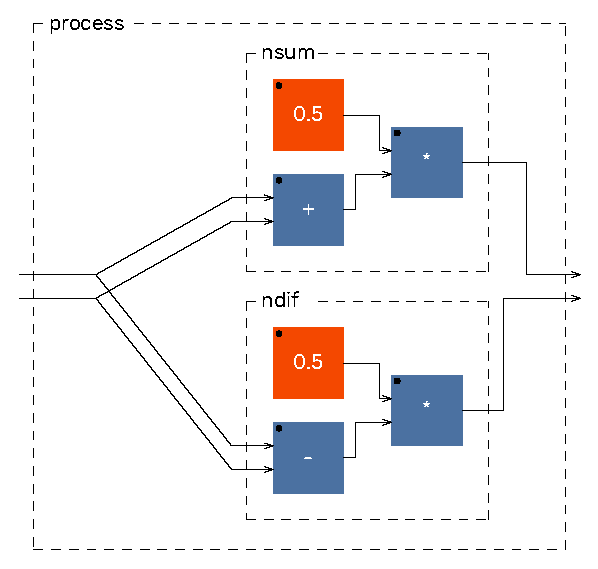
\includegraphics[]{CAPITOLI/1000/IMG/sdmx}
  \caption{Matrice somma e sottrazione.}
  \label{bd:sdmx}
\end{figure}

%%%%%%%%%%%%%%%%%%%%%%%%%%%%%%%%%%%%%%%%%%%%%%%%%%%%%%%%%%%%%%%%%%%% SECTION SIX
%%%%%%%%%%%%%%%%%%%%%%%%%%%%%%%%%%%%%%%%%%%%%%%%%%%%%%%%%%%%%%%%%%%%%%%%%%%%%%%%
\subsection{Mid-Side \emph{mic}}
\label{subsec:msmic}

\begin{figure}[b!]
\centering
\includegraphics[width=0.99\columnwidth]{CAPITOLI/_TIKZ/POLAR/midside}
\caption{Rappresentazione ideale della coppia stereofonica Mid-Side costituita da
da un microfono direzionale cardioide a gradiente di pressione mediante la sua
equazione polare: $cpg = 0.5(x) + 0.5(x\cos\theta)$ (\emph{cardioid pressure
gradient}) e da un microfono bidirezionale a gradiente di
pressione mediante la sua equazione polare: $bpg = x\cos\theta$
(\emph{bidirectional pressure gradient}). Nella tecnica microfonica di registrazione
Mid-Side il microfono cardioide convenzionalmente viene registrato nel primo canale,
mentre il segnale del microfono bidirezinale viene registrato nel secondo canale.}
\label{polar:midsidemic}
\end{figure}

La produzione di un segnale \emph{Mid-Side} come quello in uscita dalla matrice
somma e sottrazione può essere ottenuta dal posizionamento diretto di una coppia
di microfoni aventi caratteristiche polari adeguate. Il segnale \emph{Mid} è
generalmente prodotto da un microfono direzionale cardioide puntato verso il fronte
stereofonico, mentre il segnale \emph{Side} è generato da un microfono
bidirezionale puntato lateralmente, offrendo al fronte il punto di massimo
annullamento. I due microfoni devono essere allineati verticalmente in modo da
risultare orizzontalmente coincidenti.


%%%%%%%%%%%%%%%%%%%%%%%%%%%%%%%%%%%%%%%%%%%%%%%%%%%%%%%%%%%%%%%%%%%% SECTION SIX
%%%%%%%%%%%%%%%%%%%%%%%%%%%%%%%%%%%%%%%%%%%%%%%%%%%%%%%%%%%%%%%%%%%%%%%%%%%%%%%%
\subsection{Mid-Side \emph{panner}}
\label{subsec:mspanner}

La coppia stereofonica di segnali \emph{Mid-Side} è stata descritta finora come
risultante della matrice somma e sottrazione applicata ad un segnale stereofonico
oppure come segnale prodotto da una coppia di microfoni aventi caratteristiche
oppurtune. Analizziamo ora un terzo sistema in grado di generare una coppia
\emph{Mid-Side} attraverso un sistema di panning.

Il canale frontale \emph{Mid} è comunemente descritto da un microfono cardioide.
Sappiamo che la componente cardioide, come moltre altre figure polari, può
essere risultante da una combinazine misurata di
componenti non-direzionale e bidirezionale.

\begin{equation}
m(x,p,\theta) = (p*x) + ((1-p)*(x\cos\theta)
\label{eq:mid}
\end{equation}

Dove $x$ è il segnale di ingresso, $p$ è il coefficiente di ampiezza che regola
il rapporto di peso tra le due componenti, $0.5$ per ottenere la figura polare
cardioide, $\theta$ è la direzione di impatto angolare espressa in radianti.

La componente \emph{Side} è costituita dalla sola componente bidirezionale.

\begin{equation}
s(x,\theta) = x*(sin(\theta))
\label{eq:side}
\end{equation}

Il codice \emph{Faust} per la costruzione di un \emph{Mid-Side Panner} è
molto simile alle equazioni che descrivono le due figure polari.

%--------------------------------------------
%----------------larghezza massima del codice
\begin{lstlisting}
mspan(x,p,rad) = m,s
with{
  m = (p*x)+((1-p)*(x*cos(rad)));
  s = x*(sin(-rad));
};
\end{lstlisting}

I due segnali in uscita dal panner non possono essere inviati direttamente ad un
sistema di ascolto basato sui due canali sinistra-destra, devono necessariamente
passarli attraverso la matrice somma e differenza ottenere ciò che Blumlein
descrive come la differenza di ampiezza nei segnali degli altoparlanti
ottenuta dalle differenze di fase.

% %--------------------------------------------
% %----------------larghezza massima del codice
% \begin{lstlisting}
% mspan_lr(x,p,rad) = mspan(x,p,rad) : sdmx;
% \end{lstlisting}

\begin{figure}[t]
\centering
\includegraphics[width=0.99\columnwidth]{CAPITOLI/1000/IMG/mspan}
\caption{Mid-Side \emph{panner}. Il grafico mostra la risposta del \emph{panner} ad una
variazione di 360 gradi da sinistra (-180 gradi) a destra (180 gradi). La linea
rossa mostra la bipolarità del segnale correlata alle informazioni angolari. La
linea blu descrive variazioni di ampiezza (sempre con fase positiva) in
relazione alle informazioni angolari. Il grafico mostra l'evidenza della percezione
zero su entrambi gli estremi $\pm180$ gradi, dove cardioide e figura-8 si annullano.}
\label{fig:mspan}
\end{figure}

% La procedura di costruzione dell'algoritmo del \emph{Mid-Side Panner} è completa.
% Il seguente codice di \emph{Faust} descrivo il panner completo di interfaccia
% grafica.

%-----------------------------------------------------------
%-------------------------------larghezza massima del codice
\begin{lstlisting}
//----------------------------------- DEGREES TO RADIANS ---
deg2rad = *(ma.PI/180);
//----------------------------------------------- PANPOT ---
rad = vslider("[02]Azimuth[style:knob]", 0,-180,180,0.1) :
      deg2rad : si.smoo;
//--------------------------------------------- P FACTOR --–
p = vslider("[01]P[style:knob]", 0.5,0,1,0.01) : si.smoo;
//--------------------------------------------- MID-SIDE --–
midside(x,p,rad) = m,s
  with{
    m = (p*x)+((1-p)*(x*cos(rad)));
    s = x*(sin(-rad));
};
//-------------------------------- MS MATRIX DESCRIPTION ---
nsum = 0.5*(_+_);
ndif = 0.5*(_-_);
sdmx = _,_ <: nsum, ndif;
//----------------------------------------- MS2LR MATRIX ---
mspan_lr(x,p,rad) = midside(x,p,rad) : sdmx;
process = os.osc(1000), p, rad : mspan_lr;
\end{lstlisting}


\section{Stereo Pairs}

\begin{quote}
Pur sottolineando l’estrema varietà di combinazioni possibili nell’uso dei
microfoni, sia per registrare che per amplificare, è di fondamentale importanza
un’analisi delle varie configurazioni di coppie stereofoniche perché,
soprattutto nel campo della registrazione, esse possono, e molto spesso devono,
essere considerate come il punto di partenza per l’installazione di un set-up
di registrazione.
\end{quote}

Così \index[names]{Schiavoni, Piero} Piero Schiavoni iniziava le sue lezioni
sulle coppie stereofoniche al Conservatorio S. Cecilia di Roma. Questo tipo di
ragionnamento ci riporta al principio di questo percorso sulla stereofonia:
la fisiologia dell'ascolto umano e le motivazioni del suono riprodotto.

Come chiarito da Blumlein \cite{ab58} fin dal principio, l'ascolto binaurale umano
oltre a riferire al cervello del mondo acustico circostante, sono in grado di
fornire le informazioni necessarie alla ricostruzione tridimensionale di tale
mondo.


Naturalmente, per quanto possano
essere tecnologicamente avanzati, i microfoni non potranno neanche lontanamente
eguagliare la perfezione dell’udito umano, che si avvale di qualche millennio
di “affinamento” evolutivo, nondimeno un corretto uso delle varie tecniche di
ripresa stereofonica è il mezzo per portarci quanto più vicino possibile al
lavoro compiuto internamente dal nostro apparato uditivo.

Attraverso una buona tecnica di ripresa stereofonica è possibile ricostruire nel
nostro cervello un’immagine sonora che si avvicini alla percezione reale, e
trasmettere nel miglior modo possibile il contenuto culturale ed emozionale
dell’evento musicale. Occorre inoltre tenere ben presente che il giudizio finale
dell’orecchio dipende in gran misura dal sistema di ascolto della registrazione,
per cui un ascolto effettuato con cuffia avrà una resa sensibilmente diversa d
quello effettuato con diffusori, per problemi ben precisi di psicoacustica, di
cui accenneremo in seguito. Il sistema di ascolto di riferimento è generalmente
quello con diffusori, in cui il punto di ascolto, naturalmente centrale rispetto
alla coppia di altoparlanti, è situato al vertice di un angolo di sessanta gradi.

\subsection{Parametri di valutazione}

Una ripresa stereofonica può essere valutata sotto diversi aspetti, ognuno dei
quali costituisce, nell'osservazione della stereofonia, un parametro d’ascolto:

\begin{compactitem}
\item localizzazione
\item definizione timbrica
\item profondità
\item spaziosità
\end{compactitem}

\begin{figure}[th]
\centering
\includegraphics[width=0.99\columnwidth]{CAPITOLI/1000/IMG/localizzazione}
\caption[]{Ripresa di un fronte sonoro e localizzazione}
\label{fig:localizzazione}
\end{figure}

\subsection{Localizzazione}

La localizzazione è la capacità della ripresa di riprodurre una posizione degli
strumenti nello spazio orizzontale (da sinistra a destra) che si avvicini il più
possibile a quella originaria. Nella fig. \ref{fig:localizzazione} vediamo nella
parte superiore una coppia che riprende un fronte sonoro ipotetico di $90°$, e
in questo fronte sono evidenziati, oltre agli estremi (A e E), alcuni punti
intermedi (centro-sinistra B, centro C e centro-destra D). Nella parte inferiore
a differenti tecniche di ripresa, corrispondono differenti risultati di
percezione della localizzazione attraverso il riascolto con un sistema
stereofonico di diffusori: alcuni di questi si avvicinano in modo soddisfacente
alla riproduzione della posizione originaria, altri (ad es. la coppia coincidente
angolata di 90°) denotano una riproduzione ristretta, tendente a centrare i
suoni, altri (ad es. la coppia omni spaziata di 3 mt.) presentano, all’opposto,
una separazione eccessiva tra i canali ed un conseguente “buco” nel centro
d’ascolto.

\subsection{La definizione timbrica}

La definizione timbrica è dovuta in gran parte alla capacità di riprodurre la
gamma di frequenze originaria senza coloriture e senza perdite. Dando per
scontato l’utilizzo di microfoni professionali in cui l’accuratezza della
risposta in frequenza sia di livello adeguato, bisogna notare che il risultato
relativo a questo parametro dipende da diversi fattori: dalla caratteristica
polare del microfono stesso, dall’angolazione tra questo e la fonte sonora, e
dalla possibile influenza delle riflessioni dovute all’ambiente che possono, per
effetti di cancellazione di fase, alterare la risposta in frequenza del microfono
producendo colorazioni e buchi nella linearità della stessa.

\subsection{La profondità}

La profondità della ripresa non è altro se non la possibilità di distinguere,
all’interno del gruppo orchestrale, differenti piani sonori, come è nella realtà,
per cui gli archi devono risultare in un piano più ravvicinato rispetto ai legni,
collocati immediatamente alle spalle dei primi, e questi devono essere a loro
volta collocati davanti agli ottoni e alle percussioni. Naturalmente eventuali
solisti avranno la precedenza nei confronti della massa orchestrale, a meno che,
come nel caso delle riprese di opere liriche, si desideri mantenere il rapporto
scenico, con le voci più lontane rispetto all’orchestra. In mancanza della
definizione di questa dimensione, il problema può essere quello di un appiattimento
dell’orchestra su un piano orizzontale, con il risultato di una ripresa, magari
buona dal punto di vista degli altri parametri, ma poco interessante e coinvolgente.

\subsection{La spaziosità}

La spaziosità della ripresa consiste nella capacità di riproduzione dell’ambiente
in cui si effettua la ripresa, quindi una registrazione che voglia tener conto
di questo parametro conterrà una certa dose del riverbero ambientale presente
nella sala. Naturalmente, la misura del riverbero ambientale dovrà essere dosata,
oltre che dall’esperienza e dal gusto, dall’attenzione che deve essere posta nell
salvaguardia della definizione timbrica dello strumento. Anche qui, il risultato
dipenderà da diversi fattori: l’acustica della sala innanzitutto, e poi la scelta
della configurazione, nonché il posizionamento della coppia stessa. Un
posizionamento molto vicino allo strumento (o al gruppo orchestrale) darà un
rapporto suono diretto/suono riverberato più favorevole al suono diretto, rispetto
ad un posizionamento della coppia ad una certa distanza.

\subsection{Tipologie di coppie stereofoniche}

Entrando più in dettaglio sulle tipologie di configurazione, e partendo dal
presupposto di avere a disposizione due microfoni della stessa marca e dello stesso
modello e con caratteristiche simili (risposta in frequenza, curva polare, ecc.),
possiamo dividere le coppie in tre categorie:

\begin{compactitem}
\item coppie coincidenti
\item coppie quasi-coincidenti
\item coppie spaziate
\end{compactitem}

\subsection{Coincidenti}

Le coppie coincidenti, comunemente note come XY, consistono in due microfoni i
cui diaframmi di ripresa siano esattamente sovrapposti, in una vista ortogonale
dall’alto, una volta posti di fronte alla sorgente sonora. Una caratteristica
comune a tutte le coppie coincidenti è che offrono in assoluto la migliore
compatibilità mono, vale a dire che nel momento in cui si vadano a sommare i du
canali si hanno i minori fenomeni di cancellazione dovuti alle differenze di fase
dei due segnali.

\subsubsection{Blumlein}

Il primo esempio è dato dalla coppia coincidente figura-8 angolata di $90°$,
cioè la cosiddetta configurazione Blumlein, (a cui ci si riferisce come
inventore della stereofonia e di alcune tecniche di ripresa stereofonica). Come
si può vedere nella fig. 3, mentre il microfono corrispondente al canal
sinistro prende la parte sinistra dell’orchestra, per effetto della configurazione
a 8 prende anche l’ambiente retrostante destro, e inversamente farà l’altro canale.
Concettualmente, questa configurazione può essere pensata anche per quello che
ciascuno dei microfoni non prende (il sinistro non prende nulla del lato destro
dell’orchestra, coincidente col punto di annullamento massimo, e ugualmente
l’altro canale). Questa configurazione rimane una delle più precise come
equilibrio tra tutti i parametri sopra descritti.

Nella configurazione Blumlein è importante che il “fronte sonoro” sia contenuto
nell’apertura a 90° della coppia, per evitare l’influenza degli spostamenti di
fase dovuti al suono catturato dai microfoni nelle rispettive zone retrostanti.

\subsubsection{XY}

Usando due cardioidi in coppia coincidente, è possibile variare la loro
angolatura, così avremo una coppia angolata a $180°$, che darà una buona
localizzazione, a scapito di una scarsa definizione nella zona centrale,
dovuta al fenomeno per cui i suoni fuori-asse si attenuano nelle componenti più
acute, ed è una configurazione da tenere presente nel caso il fronte sonoro
sia limitato in ampiezza e si desideri avere una grande apertura sul
riverbero ambientale.

Angolando i microfoni a $135°$, avremo un miglioramento
della definizione, perché le curve polari, riducendo l’angolatura, tendono
sommare le risposte. Questa coppia ha una minore apertura stereo, è può essere
utilizzata quando si voglia raggiungere questo risultato.

Riducendo ancora l’angolatura, abbiamo la coppia angolata a $90°$ che, come
evidenziato nella tabella di fig. \ref{fig:localizzazione}, è la configurazione
che presenta la più ridotta apertura stereo, tendendo a concentrare i suoni
verso il centro. Può essere desiderabile quando il fronte sonoro è molto ampio
e si sia obbligati a riprenderlo molto da vicino.

\clearpage

\begin{figure*}[t]
    \centering
    \begin{subfigure}[t]{0.99\textwidth}
        \centering
        \includegraphics[width=11cm]{microphone-polar-patterns/blumlein}
        \caption[]{BLUMLEIN. Coppia stereofonica coincidente di figura-8 angolati tra loro di $90°$.}% \\ Eq: $1(x)$}
        \label{pol:blumleinsp}
    \end{subfigure}%
    \\
    \begin{subfigure}[t]{0.99\textwidth}
        \centering
        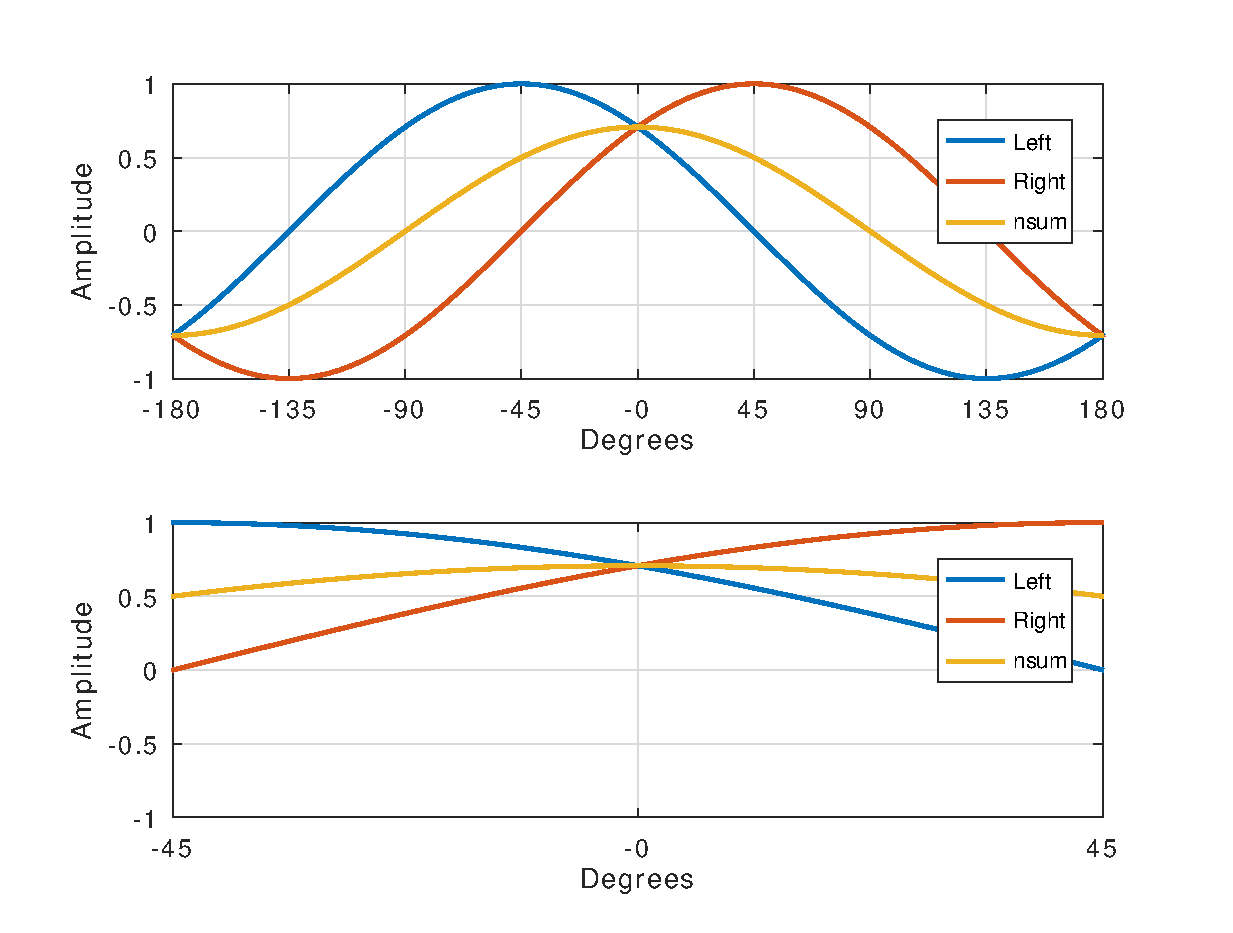
\includegraphics[width=12.5cm]{CAPITOLI/1000/IMG/blumleinsub}
        \caption[]{Variazioni angolari di ampiezza.}% \\ Eq: $0.75(x)+0.25(x\cos\theta)$}
        \label{plot:blumlein}
    \end{subfigure}
    \caption[]{BLUMLEIN}
    \label{sp:blumlein}
\end{figure*}

\clearpage

\begin{figure*}[t]
    \centering
    \begin{subfigure}[t]{0.99\textwidth}
        \centering
        \includegraphics[width=11cm]{microphone-polar-patterns/xy180}
        \caption[]{XY90. Coppia stereofonica coincidente di cardioidi angolati tra loro di $180°$.}% \\ Eq: $1(x)$}
        \label{pol:xy120sp}
    \end{subfigure}%
    \\
    \begin{subfigure}[t]{0.99\textwidth}
        \centering
        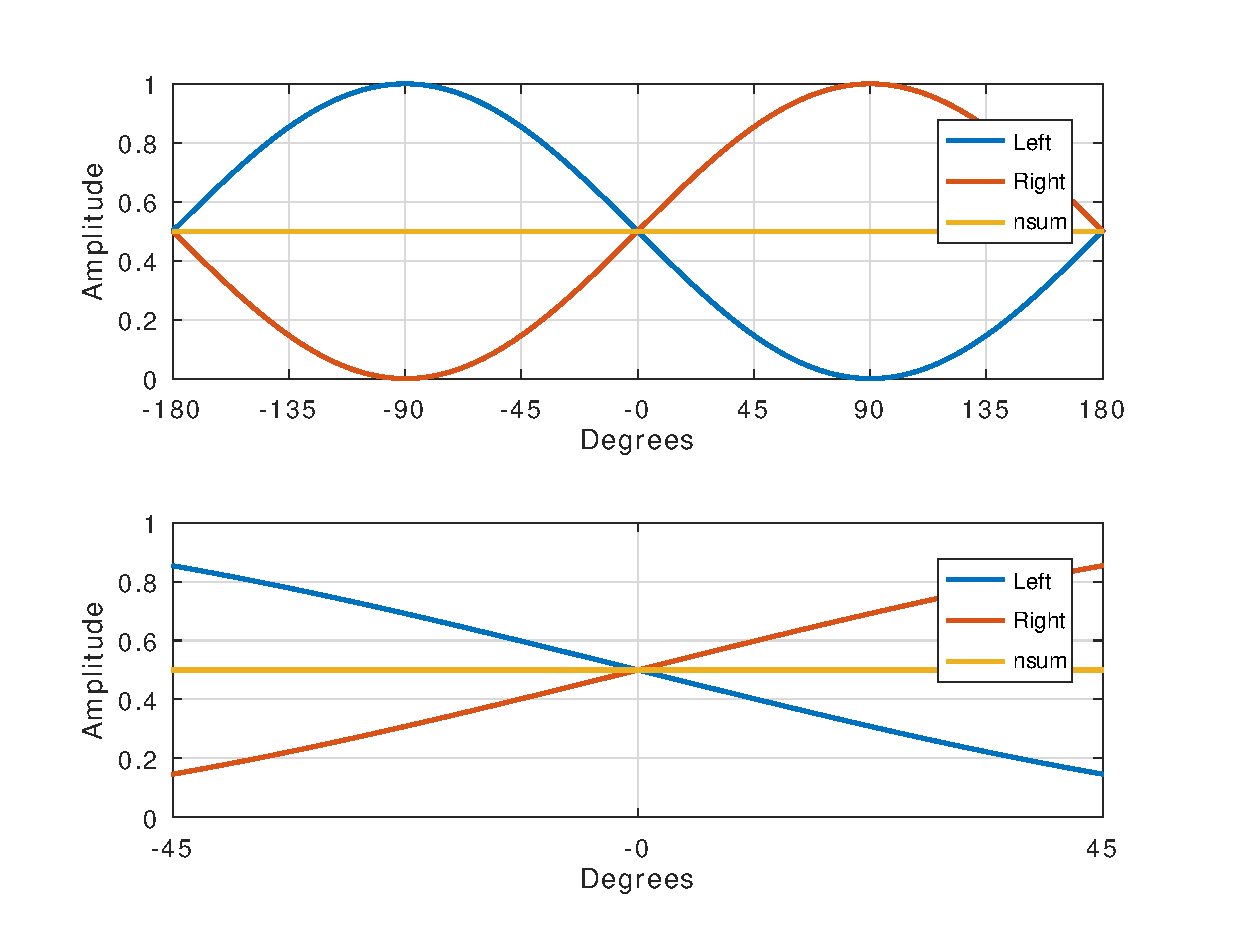
\includegraphics[width=12.5cm]{CAPITOLI/1000/IMG/xy180sub}
        \caption[]{Variazioni angolari di ampiezza.}% \\ Eq: $0.75(x)+0.25(x\cos\theta)$}
        \label{plot:xy180}
    \end{subfigure}
    \caption[]{XY180}
    \label{sp:xy180}
\end{figure*}

\clearpage

\begin{figure*}[t]
    \centering
    \begin{subfigure}[t]{0.99\textwidth}
        \centering
        \includegraphics[width=11cm]{microphone-polar-patterns/xy120}
        \caption[]{XY90. Coppia stereofonica coincidente di cardioidi angolati tra loro di $120°$.}% \\ Eq: $1(x)$}
        \label{pol:xy120sp}
    \end{subfigure}%
    \\
    \begin{subfigure}[t]{0.99\textwidth}
        \centering
        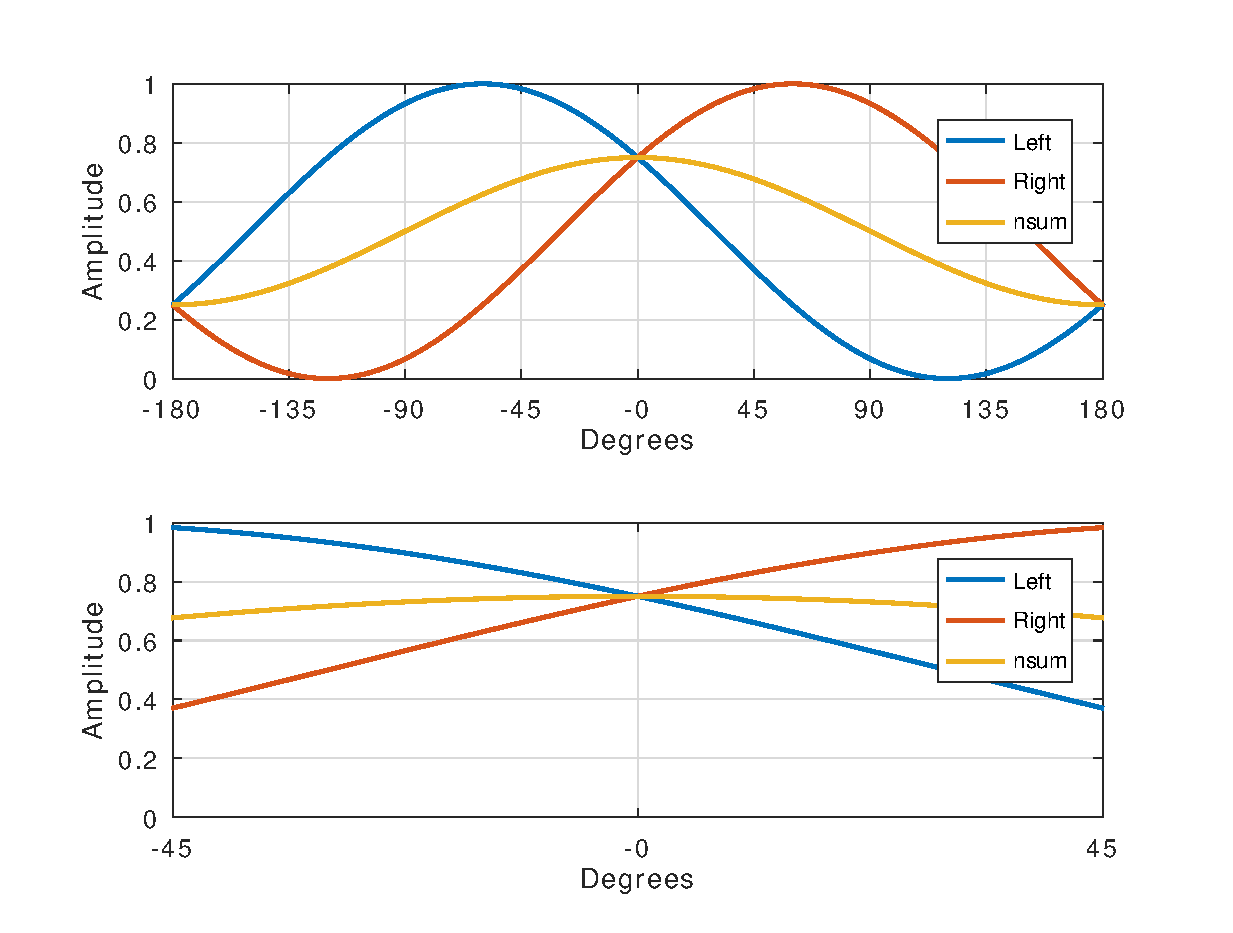
\includegraphics[width=12.5cm]{CAPITOLI/1000/IMG/xy120sub}
        \caption[]{Variazioni angolari di ampiezza.}% \\ Eq: $0.75(x)+0.25(x\cos\theta)$}
        \label{plot:xy120}
    \end{subfigure}
    \caption[]{XY120}
    \label{sp:xy120}
\end{figure*}

\clearpage

\begin{figure*}[t]
    \centering
    \begin{subfigure}[t]{0.99\textwidth}
        \centering
        \includegraphics[width=11cm]{microphone-polar-patterns/xy90}
        \caption[]{XY90. Coppia stereofonica coincidente di cardioidi angolati tra loro di $90°$.}% \\ Eq: $1(x)$}
        \label{pol:xy90sp}
    \end{subfigure}%
    \\
    \begin{subfigure}[t]{0.99\textwidth}
        \centering
        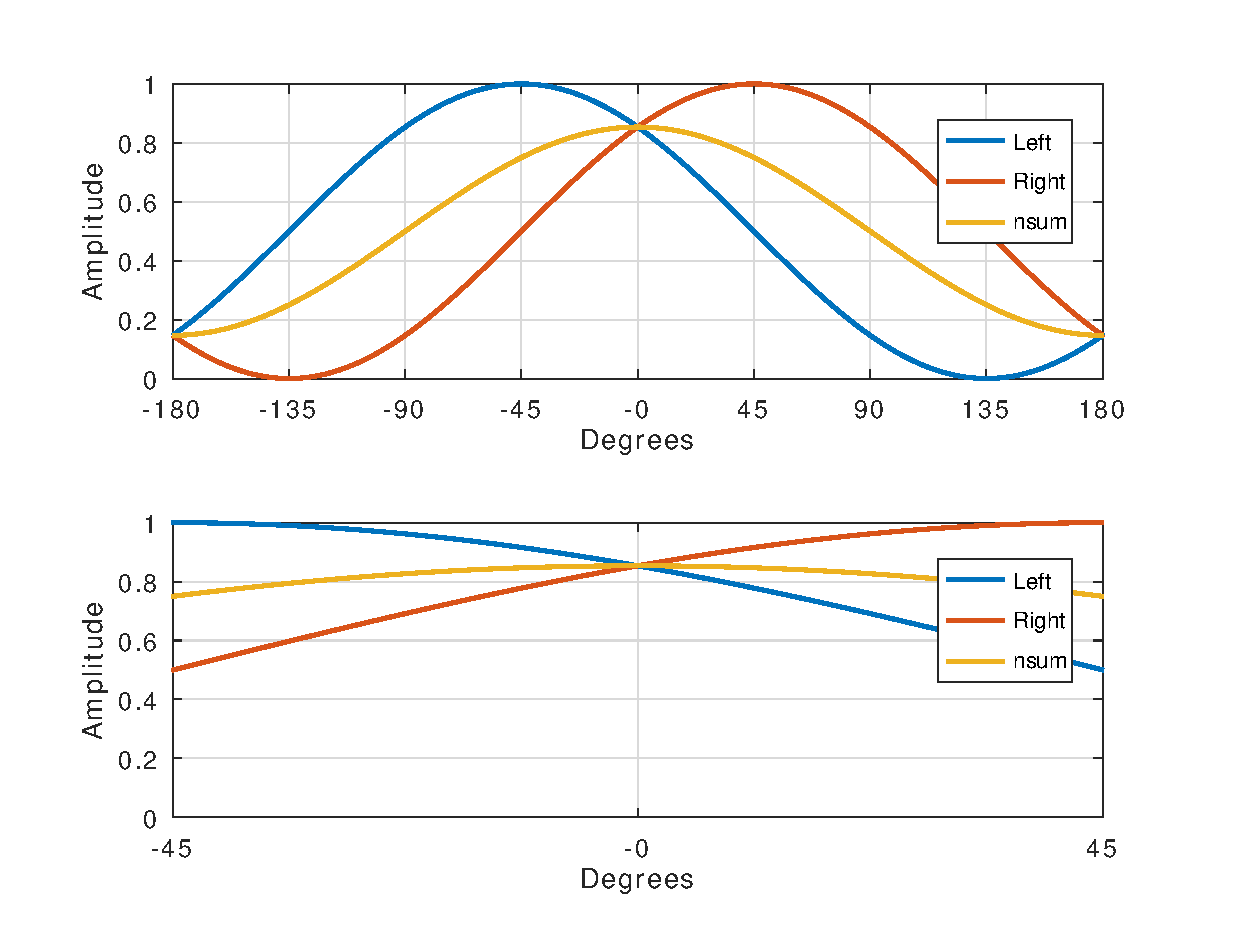
\includegraphics[width=12.5cm]{CAPITOLI/1000/IMG/xy90sub}
        \caption[]{Variazioni angolari di ampiezza.}% \\ Eq: $0.75(x)+0.25(x\cos\theta)$}
        \label{plot:xy90}
    \end{subfigure}
    \caption[]{XY90}
    \label{sp:xy90}
\end{figure*}

\clearpage

\subsection{Semi-coincidenti}

Le coppie quasi-coincidenti, rispetto a quelle esaminate fin qua, offrono una
maggiore ampiezza di immagine stereofonica ed una resa più ricca della riverberazione
ambientale. Per converso, diminuisce la compatibilità mono, in quanto allontanando
tra loro i diaframmi dei microfoni diminuisce la coerenza di fase, in special
modo alle alte frequenze.

Nella fig. \ref{pol:ortfsp} è illustrata una coppia angolata di $110°$ e spaziata
di $17cm$, la cosiddetta coppia ORTF, dal nome dell’allora ente radiotelevisivo
francese all’interno del quale è stata sviluppata. Può essere considerata i
assoluto come una delle migliori soluzioni per tutti i parametri sopra illustrati.

Un’altra coppia quasi-coincidente, la configurazione “DIN”, dove l’angolatura
è stata ridotta a 90° e la distanza tra le capsule portata a 20 cm. Come si può
constatare dalla tabella di fig. \ref{fig:localizzazione}, questo porta a
spostare verso il centro i suoni intermedi e ad allargare i suoni estremi.
Se la distanza viene portata a 30 cm la configurazione prende il nome di “NOS”.

\clearpage

\begin{figure*}[t]
    \centering
    \begin{subfigure}[t]{0.99\textwidth}
        \centering
        \includegraphics[width=11cm]{microphone-polar-patterns/ORTF}
        \caption[]{ORTF. Coppia stereofonica semi-coincidente di cardioidi angolati tra loro di $110°$ e distanti $17cm$.}% \\ Eq: $1(x)$}
        \label{pol:ortfsp}
    \end{subfigure}%
    \\
    \begin{subfigure}[t]{0.99\textwidth}
        \centering
        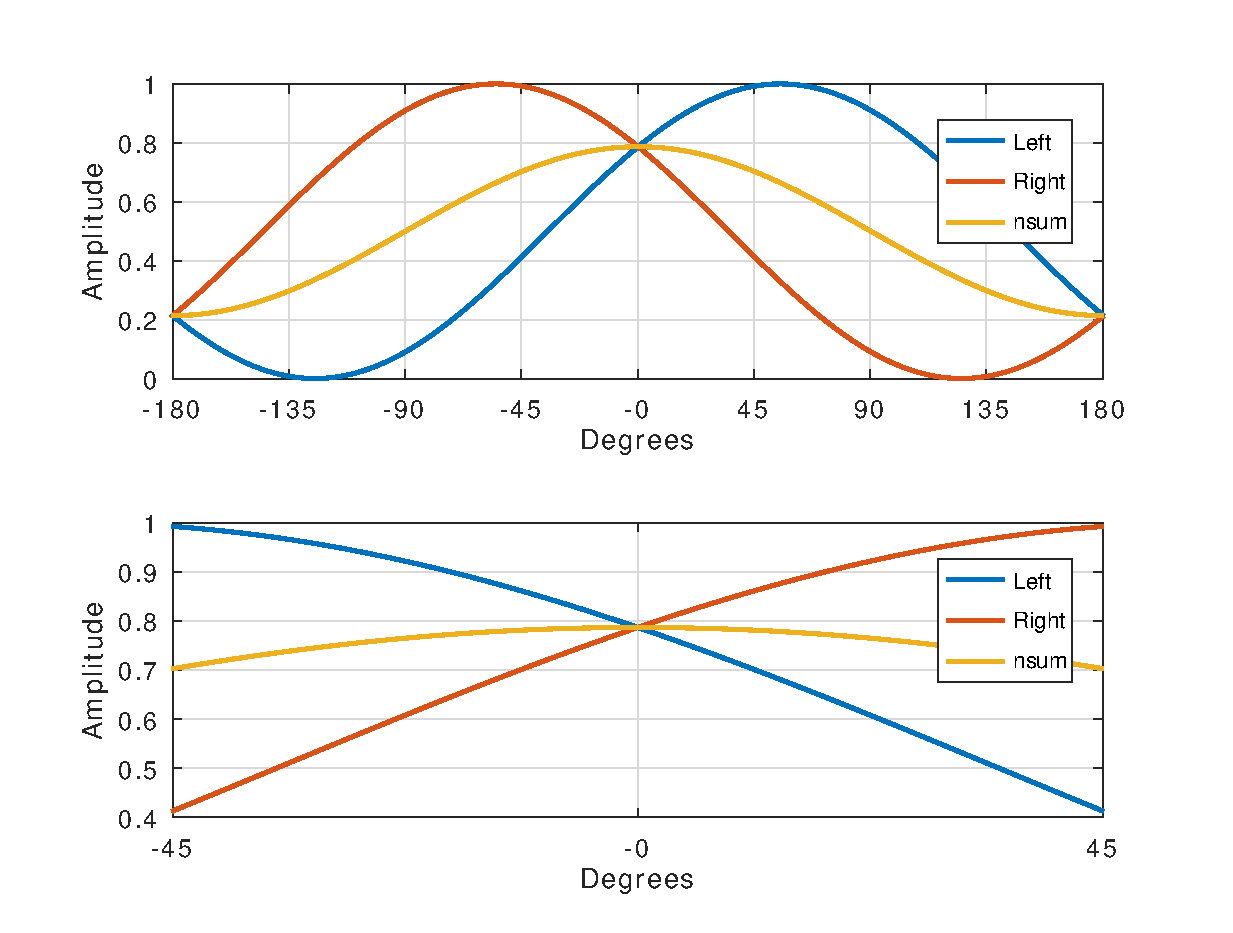
\includegraphics[width=12.5cm]{CAPITOLI/1000/IMG/ortfsub}
        \caption[]{Variazioni angolari di ampiezza.}% \\ Eq: $0.75(x)+0.25(x\cos\theta)$}
        \label{plot:ortf}
    \end{subfigure}
    \caption[]{ORTF}
    \label{sp:ortf}
\end{figure*}

\clearpage

\subsection{Le coppie spaziate}

Le coppie spaziate sono generalmente costituite da microfoni omnidirezionali
posizionati in parallelo tra di loro, rivolti verso la fonte sonora, e spaziati
di una certa distanza. Essendo entrambi i microfoni orientati nella stessa
direzione senza angolatura, la stereofonia è data dalla diversità di tempo
con cui il suono raggiunge i due microfoni, che si traduce anche in una
differenza di fase. E’ un tipo di ripresa molto adatto in ambienti dove il
riverbero ambientale è molto equilibrato, come ad es. un auditorium, in
quanto la capsula omnidirezionale riesce a restituire con ricchezza di dettaglio
anche gran parte del suono fuori asse. Altra caratteristica importante del
microfono omnidirezionale è la capacità di ripresa dei suoni gravi, superiore
a quella dei microfoni direttivi, per cui, nel caso di una registrazione
orchestrale, potrà rendere in maniera migliore suoni che si estendono molto
nella gamma bassa, come i contrabbassi, la grancassa, ecc. Va detto che tra
tutte le configurazioni è quella con la minor compatibilità mono, a causa delle
differenze di fase sopra descritte, per cui ove fosse impiegata in ripresa che
potrebbero avere un utilizzo in mono (ad es. riprese televisive), va usata con
prudenza e va controllato l’ascolto in mono per essere sicuri che non siano
avvertibili cancellazioni di fase.

%Nella fig. 10 la spaziatura è stata portata a 3 metri, e nella tabella di fig. 2 si può notare la differenza di questa ripresa rispetto alla precedente: gli strumenti tendono ad ammucchiarsi o tutti a sinistra o tutti a destra, lasciando un buco al centro.

%Nella fig. 11 nella configurazione precedente vediamo inserito un microfono centrale, che sul mixer sarà assegnato a entrambi i canali (left-right), con la funzione di ricreare il centro mancante. Questa configurazione, in realtà, non è più una coppia microfonica, essendo i microfoni tre, ma è generalmente considerata una variante delle configurazioni precedenti. In tale configurazione si usano indifferentemente sia microfoni cardioidi che omnidirezionali, e una grande cura deve essere posta nel posizionamento in vista di possibili effetti di “comb-filter” tra i tre microfoni.

Un ulteriore variante dei tre omnidirezionali è il cosiddetto “albero Decca”
(Decca tree), sviluppato dall’omonima casa discografica, dove il microfono
centrale è stato collocato in una posizione molto avanzata, in modo da dare
alla ripresa un centro assolutamente stabile, in conseguenza anche delle
differenze di tempo d’arrivo del suono. Il microfono preferito per questa
configurazione, quello con il quale questa configurazione è nata, è il
Neumann M50, ossia un microfono omnidirezionale a pressione dotato di una marcata
esaltazione delle frequenze alte in asse.

Un interessante configurazione è rappresentata dal sistema OSS (Jecklin disk),
in cui due microfoni omnidirezionali, spaziati di $16.5cm$, sono separati da un
divisorio rigido ricoperto di materiale fonoassorbente. Un tale sistema è vicino
alla simulazione di una testa umana, e può essere utile in riprese destinate
all’ascolto in cuffia (registrazioni binaurali).

Un’importante configurazione è la cosiddetta MS (mid-side), che consiste in un
microfono direzionale (cardioide o ipercardioide) sovrapposto ad un microfono
figura-8 disposto in modo da avere il punto di annullamento massimo in direzione
frontale. In tal modo, il microfono direttivo conterrà l’informazione relativa
al suono centrale (mid), mentre l’altro conterrà l’informazione relativa al
suono laterale (side).

%Il microfono mid entra in un canale e viene inviato, tramite il potenziometro panpot, ad entrambi i canali di uscita, mentre il microfono side viene fatto entrare su due canali, uno dei quali avrà il commutatore di fase invertito. Questi due canali vengono assegnati uno all’uscita sinistra e l’altro all’uscita destra, e potranno essere dosati e controllati tramite i relativi potenziometri del livello (fader). Il vantaggio di questa configurazione risiede proprio nella possibilità di separare l’informazione centrale da quella laterale, e di avere l’opportunità di controllare il bilanciamento di queste due informazioni.

%Un’ultima coppia stereofonica da segnalare è quella nota come “Testa artificiale” (Dummy Head, fig. 16), che consiste in una coppia di microfoni, generalmente omnidirezionali, installati all’interno di una struttura riproducente la conformazione di una testa umana, e posizionati in corrispondenza delle orecchie. Tale configurazione, tendente a simulare nel modo più accurato possibile la percezione umana, produce un tipo di registrazioni note come “registrazioni binaurali”, di cui tratteremo in seguito.

\subsection{Dummy Head}



\appendix

%!TEX TS-program = xelatex
%!TEX encoding = UTF-8 Unicode
% !TEX root = ../metp.tex

\chapter{Pensare il tempo}

\begin{flushright}
\textit{- Alice: How long is forever?\\
- White Rabbit: Sometimes, just one second.”}\\
Lewis Carroll, Alice in Wonderland
\end{flushright}

In questa sezione affronteremo un piccolo esercizio di programmazione che porterà
alla creazione di un semplice metronomo digitale. Lo scopo di tale esercizio è
quello di accedere alla programmazione temporizzata degli eventi sonori.

risorse necessarie:\\
\url{http://faustide.grame.fr/}

\startcontents[chapters]
\printcontents[chapters]{}{1}{}

\section{Scansioni ritmiche}

Prima di inoltrarsi nel pratico della creazione, c'è un minimo di riflessione da
fare sul come dividiamo il tempo e perché.

\begin{quote}
Da secoli, \emph{dividiamo} il tempo in giorni. La parola “tempo” deriva da una
radice indoeuropea, \emph{di} o \emph{dai}, che indica “dividere”. Da secoli,
dividiamo il giorno in ore. Per la maggior parte di questi secoli, però, le ore
erano più lunghe d'estate e più corte d'inverno, perché le 12 ore scandivano il
tempo fra alba e tramonto: l'ora prima era l'alba, e l'ora dodicesima il tramonto,
indipendentemente dalla stagione. [\ldots] È solo verso il XIII secolo che in Europa
la vita della gente comincia a essere regolata da orologi meccanici. Città e
villaggi costruiscono la loro chiesa, accanto alla chiesa il campanile, e sul
campanile un orologio che dà il ritmo alle funzioni collettive. Inizia l'era del
tempo regolato da orologi\footnote{Rovelli - l'ordine del tempo. pg 56-57}.
\end{quote}

L'idea di un tempo fluido, che non ticchetta, che non rintocca, era la consuetudine
prima degli orologi. Oggi è molto meno comune un pensiero di questo tipo. Siamo
legati ai ticchettii.
\begin{quote}
L'utilità degli orologi è indicare a tutti la stessa ora. Ma anche quest'idea è
più moderna di quanto possiamo immaginare. Per secoli, finché si viaggiava a
cavallo, a piedi o in carrozza, non c'era motivo di sincronizzare orologi da un
luogo all'altro. C'era un ottimo motivo per \emph{non} farlo: mezzodì è per
definizione quando il sole è più alto nel cielo. [\ldots] Nel XIX secolo arriva
il telegrafo, i treni diventano comuni e veloci, e il problema di sincronizzare
bene gli orologi da una città all'altra si fa importante\footnote{Rovelli - l'ordine del tempo}.
\end{quote}

Anche il metronomo ha la sua storia. Innanzitutto l'etimologia della parola,
che compare per la prima volta nel 1815 per opera di Johann Nepomuk M\"{a}lzel
mediante l'unione di due parole greche: \emph{metron}, misura e \emph{nomos}, regola.
Seppur sotto il nome di M\"{a}lzel, tanto da trovare indicazioni metronomiche
con la sigla \emph{MM} (Metronomo M\"{a}lzel), il dispositivo si basa su un
principio messo a punto da Dietrich Nikolaus Winkel, al quale M\"{a}lzel aggiunse
il tipico rintocco sonoro. Il musicista analogico sa che M\"{a}lzel e Winkel sono
rimasti a lungo due marchi importanti di metronomi meccanici.

Il metronomo meccanico si basa sui concetti dell'oscillazione pendolare:
è infatti costituito da pendolo capovolto, con un'asta graduata fra le 40 scansioni
e le 208 scansioni al minuto primo. Spostando un peso lungo l'asta graduata
selezioniamo la quantità di pulsazioni per minuto.

\section{Beat per minuto}

\emph{Quanti secondi ci sono in un minuto?} Sessanta.

\emph{Quanti minuti ci sono in un'ora?} Sessanta.

\emph{Quanti secondi ci sono in un'ora?} Tremilaseicento ($60*60$).

\emph{Quanto tempo passa tra i rintocchi di un metronomo a $108bpm$?}

L'indicazione metronomica $bpm$ \emph{(Beat per minute)} ci indica quanti rintocchi
vogliamo sentire in un minuto. Ad una quantità di $60bpm$ ascoltiamo un rintocco
sessanta volte per minuto, una scansione che corrisponde a quella dei secondi.
Il metronomo impostato a $60bpm$ produce un rintocco ogni secondo, il secondo è
la distanza che c'è tra un rintocco ed il successivo.

Il minuto è la nostra grandezza di riferimento. La nostra torta intera. Ad una
scansione di $60sec$ dividiamo, come sull'orologio, la torta in sessanta parti
uguali, e avanziamo tra una e l'altra di $1/60$ di minuto (ovvero $1sec$).
Ad una scansione di $108bpm$ (battiti per minuto) stiamo dividendo la torta in
centootto parti uguali ed avaziamo tra una parte e l'altra di $1/108$ di minuto.
Volendo individuare la distanza in secondi tra un rintocco ed il successivo non
ci resta che sostituire il minuto con l'equivalente in secondi, sessanta. La
distanza che separa un beat dal successivo ($\Delta(bpm)$) in una scansione di $108BMP$ può
essere calcolata quindi con $60/108=0,\overline{5}sec$.

\begin{equation}
\Delta(bpm) = 60/bpm (sec)
\end{equation}

Volendo aumentare il grado di precisione del calcolo precedente, ci basterà scendere
ad unità di misura più piccole del secondo, come per esempio il millesimo di secondo.

\emph{Quanti millesimi di secondo ci sono in un minuto?} Sessantamila.

\section{Metronomo}

Il metronomo digitale non può far affidamento su leggi meccaniche e masse in
movimento. Il tempo all'interno del mondo informatico si muove diversamente dagli
orologi. Per un computer non è troppo difficile portare il tempo anche in
presenza di tempi diversi, per esempio, un video multimediale può avere una scansione
di $23.976fps$ (\emph{frame per second}) e, all'interno dello stesso secondo, un suono
può avere $48000Hz$ di sample rate, ovvero essere descritto in un secondo per 48000 punti.

La frequenza di campionamento, \emph{sample rate (sr)}, nel magico mondo dei
segnali audio digitali, è la divisione del secondo per l'unità più piccola descrivibile,
il campione (\emph{sample}). Alla frequenza di campionamento di $48000Hz$ un campione
è grande $1/48000sec$. La torta, il secondo, è divisa in quarantottomila parti.

\emph{A $SR=48000$ quanti campioni ci sono in un minuto?} Due milioni e ottocentoottantamila.

Le frequenze di campionamento, seppur standardizzate, possono essere molteplici in
quanto definiscono quanto è accurata la descrizione del suono digitale nel tempo.

Dovremo riferirci ad una formula che generalizzi il valore della frequenza di campionamento
e sapere esattamente a che frequenza si esegue il calcolo, per ricavare il numero
di campioni che occorrono in ogni minuto, $spm$ (\emph{samples per minute}).

\begin{equation}
spm = SR*60
\end{equation}

Ora che il nostro orologio audio è definito nel numero di campioni che compongono
il minuto, è piuttosto semplice capire a che distanza, in campioni, avviene un
rintocco dal successivo alla velocità metronomica di $108BMP$ ad una frequenza
di campionamento di $48000Hz$, attraverso la formula $48000*60/108=26666,\overline{6}$.
È indispensabile chiarire immediatamente che per il computer non esiste, nella
descrizione del segnale audio, la parte decimale del campione, quindi di quella
dimensione terremo solo la parte intera: un rintocco ogni $26666$ campioni.

Ci sono ora i presupposti concettuali per iniziare a scrivere il codice di programma
che porterà al metronomo digitale.

%-----------------------------------------------------------
%-------------------------------larghezza massima del codice
\begin{lstlisting}
//-------------------------------------------- METRONOMO ---
//------------------------------- dichiarazioni iniziali ---
declare name "METRONOMO";
import("stdfaust.lib");
//------------------- numero di campioni per ogni minuto ---
SPM = (60*ma.SR);
\end{lstlisting}

Con le prime righe di codice abbiamo iniziato, e dato un nome, al progetto metronomo.
Il consueto \emph{import} della libreria standard ci permette di utilizzare
le funzioni standard di Faust. Con la funzione \emph{spm} otteniamo il numero di
campioni per minuto, chiendendo a Faust di verificare a che frequenza di campionamento
è impostato il computer prima di effettuare il calcolo, attraverso la funzione
matematica standard \emph{ma.SR}.

Aggiungiamo al codice precedente il selettore del valore metronomico attraverso
uno slider orizzontale

\begin{lstlisting}
//------------------------------- cursore selezione BPM ---
BPM = hslider("[01]BPM", 60, 40, 240, 0.1);
\end{lstlisting}

Ora che siamo in grado di introdurre il valore metronomico dovremo inserire
la formula che mette in relazione il numero di campioni per ogni minuto con la
quantità di BPM desiderata

\begin{lstlisting}
//-------------------------------- cursore selezione BPM ---
//-------------------- init-min--max-step-------------------
BPM = hslider("[01]BPM", 60, 40, 240, 0.1);
//------------------- numero di campioni per ogni minuto ---
SPM = (60*ma.SR);
//------------- formula di conversione da BPM a campioni ---
tempo = SPM/BPM : int; // solo la parte intera
\end{lstlisting}

Il sistema ora è in grado di fornire la distanza tra un rintocco ed il successivo
al variare dei $bpm$. Facciamolo suonare.

\begin{lstlisting}
//-------------------------------------------- METRONOMO ---
//------------------------------- dichiarazioni iniziali ---
declare name "METRONOMO";
import("stdfaust.lib");
//-------------------------------- cursore selezione BPM ---
//-------------------- init-min--max-step-------------------
BPM = hslider("[01]BPM", 60, 40, 240, 0.1);
//------------------- numero di campioni per ogni minuto ---
SPM = (60*ma.SR);
//------------- formula di conversione da BPM a campioni ---
tempo = SPM/BPM : int; // solo la parte intera
//--------------------------------- impulso temporizzato ---
metronomo = ba.pulsen(1, tempo); // (dimensione - distanza)
//------------------- METRONOMO SUI DUE CANALI DI USCITA ---
process =   metronomo <: _,_ ;
\end{lstlisting}

Il sistema funziona, agendo sul controllo BPM otteniamo quello la variazione di
distanza tra i rintocchi.

L'oggetto \emph{ba.pulsen} produce una pulsazione ad intervalli regolari.
La pulsazione può essere di grandezza variabile, così come la distanza, entrambe
le grandezze espresse in campioni. La riga

\begin{lstlisting}
//--------------------------------- impulso temporizzato ---
metronomo = ba.pulsen(1, tempo); // (dimensione - distanza)
\end{lstlisting}

genera un impulso grande un campione alla distanza in campioni espressa da \emph{tempo}
che sappiamo produrre il numero di campioni in relazione al numero di $bpm$ immesso.
L'impulso grande un campione è un clik unitario, ovvero grande la dimensione
più piccola possibile in un segnale audio ed è definito impulso.
Un impulso di questo tipo, se osservato nel dominio della frequenza contiene tutte
le frequenze dello spettro audio. In questo senso, un segnale contenente ogni
frequenza della banda audio, sprigionata in un impulso, è il segnale perfetto per
far risuonare un filtro, esattamente come farebbe una campana colpita da un martello.
A parità di martello e di energia, più la campana sarà stretta, più sarà lunga la risonanza.

\begin{lstlisting}
//---------------------------------------------- SINTESI ---
//------------------------------------- filtro risonante ---
fireson = fi.highpass(128, 1000) : fi.lowpass(8, 1000);
\end{lstlisting}

Il primo filtro è un filro passa alto del centoventottesimo ordine, intonato a
$1000Hz$ e si comporta come una campana intonata a quella frequenza. Il secondo
filtro è opposto, passa basso, serve a tenere sotto controllo la banda passante nel
versante superiore ed elimina il suono impulsivo iniziale.

Il metronomo è ora completo, di seguito il codice contenente tutti i passaggi
precedenti\footnote{Il codice completo può essere compilato online e scaricato
sul computer o direttamente sul proprio smartphone puntando il \emph{QRcode}.}.

%-----------------------------------------------------------
%-------------------------------larghezza massima del codice
\begin{lstlisting}
//-------------------------------------------- METRONOMO ---
//------------------------------- dichiarazioni iniziali ---
declare name "METRONOMO";
import("stdfaust.lib");
//-------------------------------- cursore selezione BPM ---
//-------------------- init-min--max-step-------------------
BPM = hslider("[01]BPM", 60, 40, 240, 0.1);
//------------------- numero di campioni per ogni minuto ---
SPM = (60*ma.SR);
//------------- formula di conversione da BPM a campioni ---
tempo = SPM/BPM : int; // solo la parte intera
//---------------------------------------------- SINTESI ---
//------------------------------------- filtro risonante ---
fireson = fi.highpass(128, 1000) : fi.lowpass(8, 1000);
//------------------------------------ impulso risonante ---
metronomo = ba.pulsen(1, tempo) : fireson;
//-------------------- METRONOMO SU DUE CANALI DI USCITA ---
process =   metronomo <: _,_ ;
\end{lstlisting}


%\clearpage

%\begin{longtable}{r|L{0.71\textwidth}}
  \multicolumn{2}{c}{\textbf{CLASSE V LICEO MUSICALE • I Quadrimestre}} \\
  \multicolumn{2}{c}{\textbf{I modulo Titolo: Linguaggi di programmazione, interattività e multimedialità}} \\
  \endhead
  \hline
  \textbf{Obiettivi} &
  \textbf{Conoscenze:} \newline
    Acquisire i principali strumenti critici per l'analisi dell'audiovisivo.\newline
    Conoscere le principali tecniche di produzione e post-produzione audio e musicale in relazione all'audiovisivo.\newline
    Completare la conoscenza del percorso storico della musica elettroacustica, le aree territoriali, i compositori e le relazioni storiche tra essi.\newline
    Principi di interattività, installazione, realtà virtuale, multimedialità. \newline
  \textbf{Abilità:} \newline
    Lettura e comprensione di testi della letteratura specifica, manuali operativi e utente, di strumenti di lavoro, hardware e software.\newline
    Elaborazione e produzione di progetti compositivi, sia in forma di esercizio che di produzione autonoma, in lavori di gruppo con sistemi di condivisione dati e networking.\newline
    Accesso alla stesura di strutture musicali per gli audiovisivi e le opere interattive.\newline
    Elaborazione e produzione di un repertorio elettroacustico.\newline
  \textbf{Competenze:} \newline
    Completa padronanza della terminologia specifica, degli strumenti di studio, esercizio e lavoro applicato alle tecnologie musicali.\newline
    Completa autonomia critica ed analitica di opere elettracustiche e digitali.\newline
    Completa autonomia di produzione ed elaborazione personale spontanea e su commissione. \\
  \hline
  \textbf{Contenuti} &
    La tecnologia come strumento di esercizio e lavoro applicato alle
    discipline di studio. L'approfondimento teorico e la prova sperimentale
    come approccio d'indagine. Il repertorio musicale e la letteratura come
    guida tra le tematiche d'approfondimento. \newline
    Il computer come strumento e ambiente di lavoro polifunzionale.
    Il linguaggio di programmazione come strumento di pensiero. \newline
    L'elaborazione dei suoni al computer, elaborazione strutturata di un segnale,
    le tecniche di \emph{digital signal processing - dsp}.\newline
    La notazione musicale contemporanea, suono segno ed interpretazione.\newline
    Le superfici di controllo, le automazioni i sensori, strutturazione e
    programmazione di un proprio ambiente di lavoro personalizzato. \\
  \hline
  \textbf{Metodo} &
    Lezione frontale in laboratorio. \newline
    Ogni tematica è affrontata accedendovi dal repertorio musicale.
    Si ascolta, analizza e comprende il brano di repertorio ed attraverso
    la sua applicazione musicale si approfondiscono gli argomenti emergenti.
    Si veicola quindi lo studio teorico e tecnico attraverso la pratica
    musicale, senza perdere il collegamento con il repertorio storico.
    Ogni fenomeno uditivo, percettivo e tecnologico è radicato nella
    musica del suo tempo, acquisibile mediante l'analisi, l'interpretazione
    e la pratica dello strumento tecnologico musicale. \\
  \hline
  \textbf{Tempi} &
    Mesi da Settembre a Gennaio\\
  \hline
  \textbf{Materiali} &
    Dispense, Estratti di testi in letteratura, partiture del repertorio,
    contenuti multimediali. \\
  \hline
  \textbf{Tipologia della verifica} &
    Prove pratiche sulle attività svolte durante i laboratori. \newline
    Questionari di diversa tipologia. \newline
    Verifiche orali.
\end{longtable}%

\clearpage

\begin{longtable}{r|L{0.71\textwidth}}
  \multicolumn{2}{c}{\textbf{CLASSE V LICEO MUSICALE • II Quadrimestre}} \\
  \multicolumn{2}{c}{\textbf{II modulo Titolo: Musicista e Tecnologia, competenze trasversali.}} \\
  \endhead
  \hline
  \textbf{Obiettivi} &
    \textbf{Conoscenze:} \newline
      Acquisire i principali strumenti critici per l'analisi dell'audiovisivo.  \newline
      Conoscere le principali tecniche di produzione e post-produzione audio e musicale in relazione all'audiovisivo.  \newline
      Completare la conoscenza del percorso storico della musica elettroacustica, le aree territoriali, i compositori e le relazioni storiche tra essi.  \newline
      Conoscenza delle pratiche di interattività, installazione, realtà virtuale, multimedialità.  \newline
    \textbf{Abilità:} \newline
      Elaborazione e produzione di progetti compositivi, relazioni, articoli scientifici e documentazione operativa, partiture e schede tecniche. \newline
      Elaborazione e produzione di strutture musicali per gli audiovisivi e le opere interattive.\newline
      Elaborazione e produzione di un repertorio elettroacustico. \newline
    \textbf{Competenze:} \newline
      Completa padronanza della terminologia specifica, degli strumenti di studio, esercizio e lavoro applicato alle tecnologie musicali. \newline
      Completa autonomia critica ed analitica di opere elettracustiche e digitali. \newline
      Completa autonomia di produzione ed elaborazione personale spontanea e su commissione. \\
    \hline
    \textbf{Contenuti} &
      La tecnologia come strumento di esercizio e lavoro applicato alle
      discipline di studio. L'approfondimento teorico e la prova sperimentale
      come approccio d'indagine. Il repertorio musicale e la letteratura come
      guida tra le tematiche d'approfondimento. \newline
      Il computer come strumento e ambiente di lavoro polifunzionale. \newline
      Il linguaggio di programmazione come strumento di pensiero. \newline
      L'elaborazione dei suoni al computer, elaborazione strutturata di un segnale,
      le tecniche di \emph{digital signal processing - dsp}. \newline
      La notazione musicale contemporanea, suono segno ed interpretazione. \newline
      Studio, ricerca e produzione, acquisizione dei mezzi per sviluppare il
      proprio percorso musicale. \\
    \hline
    \textbf{Metodo} &
      Lezione frontale in laboratorio. \newline
      Ogni tematica è affrontata accedendovi dal repertorio musicale.
      Si ascolta, analizza e comprende il brano di repertorio ed attraverso
      la sua applicazione musicale si approfondiscono gli argomenti emergenti.
      Si veicola quindi lo studio teorico e tecnico attraverso la pratica
      musicale, senza perdere il collegamento con il repertorio storico.
      Ogni fenomeno uditivo, percettivo e tecnologico è radicato nella
      musica del suo tempo, acquisibile mediante l'analisi, l'interpretazione
      e la pratica dello strumento tecnologico musicale. \\
    \hline
    \textbf{Tempi} &
      Mesi da Febbraio a Giugno \\
    \hline
    \textbf{Materiali} &
      Dispense, Estratti di testi in letteratura, partiture del repertorio,
      contenuti multimediali. \\
    \hline
    \textbf{Tipologia della verifica} &
      Prove pratiche sulle attività svolte durante i laboratori. \newline
      Questionari di diversa tipologia. \newline
      Verifiche orali. \newline
      Presentazione della produzione personale acquisita durante l'anno scolastico. \newline
      Prova pratica interpretazione d'insieme in forma di concerto.
  \end{longtable}%

\clearpage

\begin{longtable}{R{0.21\textwidth}|L{0.71\textwidth}}
\multicolumn{2}{c}{\textbf{CRITERIO DI SUFFICIENZA}} \\
\endhead
\hline
\multicolumn{2}{c}{L’alunno conseguirà la valutazione sufficiente quando dimostrerà di possedere:} \\
\hline
\multicolumn{2}{c}{\textbf{Nel I Quadrimestre:}} \\
\hline
Conoscenze: &
Conoscenza completa delle discipline in oggetto, del lessico specifico, degli strumenti di lavoro. \\
\hline
Abilità: &
Capacità di gestione autonoma di attività tecniche e pratiche all'interno del laboratorio, individuali e collettive. \\
\hline
Competenze: &
Competenza e lessico appropriato nel rapporto con gli strumenti di lavoro e le tecnologie. \newline
Competenza dell'ambiente virtuale al computer, dell'acquisizione e trattamento digitale dei suoni. \newline
Autonomia critica, analitica e di giudizio, d'ascolto e relazione con la musica e i media. \\
\hline
\multicolumn{2}{c}{\textbf{Nel II Quadrimestre:}} \\
\hline
Conoscenze: &
Conoscenza completa delle discipline in oggetto, del lessico specifico, degli strumenti di lavoro. \\
\hline
Abilità: &
Capacità di gestione autonoma di attività tecniche e pratiche all'interno del laboratorio, individuali e collettive. \\
\hline
Competenze: &
Competenza e lessico appropriato nel rapporto con gli strumenti di lavoro e le tecnologie. \newline
Competenza dell'ambiente virtuale al computer, dell'acquisizione e trattamento digitale dei suoni. \newline
Autonomia critica, analitica e di giudizio, d'ascolto e relazione con la musica e i media.
\end{longtable}

\clearpage


\clearpage

\printbibliography

\clearpage

\listoffigures

\clearpage

\listoftables

\clearpage

%\listofformulas

\addcontentsline{toc}{chapter}{Indice dei nomi}
\printindex[names]

\addcontentsline{toc}{chapter}{Indice analitico}
\printindex[things]

\end{document}
